% Options for packages loaded elsewhere
\PassOptionsToPackage{unicode}{hyperref}
\PassOptionsToPackage{hyphens}{url}
\PassOptionsToPackage{dvipsnames,svgnames,x11names}{xcolor}
%
\documentclass[
  us-letterpaper,
]{scrreprt}

\usepackage{amsmath,amssymb}
\usepackage{iftex}
\ifPDFTeX
  \usepackage[T1]{fontenc}
  \usepackage[utf8]{inputenc}
  \usepackage{textcomp} % provide euro and other symbols
\else % if luatex or xetex
  \usepackage{unicode-math}
  \defaultfontfeatures{Scale=MatchLowercase}
  \defaultfontfeatures[\rmfamily]{Ligatures=TeX,Scale=1}
\fi
\usepackage{lmodern}
\ifPDFTeX\else  
    % xetex/luatex font selection
\fi
% Use upquote if available, for straight quotes in verbatim environments
\IfFileExists{upquote.sty}{\usepackage{upquote}}{}
\IfFileExists{microtype.sty}{% use microtype if available
  \usepackage[]{microtype}
  \UseMicrotypeSet[protrusion]{basicmath} % disable protrusion for tt fonts
}{}
\makeatletter
\@ifundefined{KOMAClassName}{% if non-KOMA class
  \IfFileExists{parskip.sty}{%
    \usepackage{parskip}
  }{% else
    \setlength{\parindent}{0pt}
    \setlength{\parskip}{6pt plus 2pt minus 1pt}}
}{% if KOMA class
  \KOMAoptions{parskip=half}}
\makeatother
\usepackage{xcolor}
\setlength{\emergencystretch}{3em} % prevent overfull lines
\setcounter{secnumdepth}{5}
% Make \paragraph and \subparagraph free-standing
\makeatletter
\ifx\paragraph\undefined\else
  \let\oldparagraph\paragraph
  \renewcommand{\paragraph}{
    \@ifstar
      \xxxParagraphStar
      \xxxParagraphNoStar
  }
  \newcommand{\xxxParagraphStar}[1]{\oldparagraph*{#1}\mbox{}}
  \newcommand{\xxxParagraphNoStar}[1]{\oldparagraph{#1}\mbox{}}
\fi
\ifx\subparagraph\undefined\else
  \let\oldsubparagraph\subparagraph
  \renewcommand{\subparagraph}{
    \@ifstar
      \xxxSubParagraphStar
      \xxxSubParagraphNoStar
  }
  \newcommand{\xxxSubParagraphStar}[1]{\oldsubparagraph*{#1}\mbox{}}
  \newcommand{\xxxSubParagraphNoStar}[1]{\oldsubparagraph{#1}\mbox{}}
\fi
\makeatother

\usepackage{color}
\usepackage{fancyvrb}
\newcommand{\VerbBar}{|}
\newcommand{\VERB}{\Verb[commandchars=\\\{\}]}
\DefineVerbatimEnvironment{Highlighting}{Verbatim}{commandchars=\\\{\}}
% Add ',fontsize=\small' for more characters per line
\usepackage{framed}
\definecolor{shadecolor}{RGB}{241,243,245}
\newenvironment{Shaded}{\begin{snugshade}}{\end{snugshade}}
\newcommand{\AlertTok}[1]{\textcolor[rgb]{0.68,0.00,0.00}{#1}}
\newcommand{\AnnotationTok}[1]{\textcolor[rgb]{0.37,0.37,0.37}{#1}}
\newcommand{\AttributeTok}[1]{\textcolor[rgb]{0.40,0.45,0.13}{#1}}
\newcommand{\BaseNTok}[1]{\textcolor[rgb]{0.68,0.00,0.00}{#1}}
\newcommand{\BuiltInTok}[1]{\textcolor[rgb]{0.00,0.23,0.31}{#1}}
\newcommand{\CharTok}[1]{\textcolor[rgb]{0.13,0.47,0.30}{#1}}
\newcommand{\CommentTok}[1]{\textcolor[rgb]{0.37,0.37,0.37}{#1}}
\newcommand{\CommentVarTok}[1]{\textcolor[rgb]{0.37,0.37,0.37}{\textit{#1}}}
\newcommand{\ConstantTok}[1]{\textcolor[rgb]{0.56,0.35,0.01}{#1}}
\newcommand{\ControlFlowTok}[1]{\textcolor[rgb]{0.00,0.23,0.31}{\textbf{#1}}}
\newcommand{\DataTypeTok}[1]{\textcolor[rgb]{0.68,0.00,0.00}{#1}}
\newcommand{\DecValTok}[1]{\textcolor[rgb]{0.68,0.00,0.00}{#1}}
\newcommand{\DocumentationTok}[1]{\textcolor[rgb]{0.37,0.37,0.37}{\textit{#1}}}
\newcommand{\ErrorTok}[1]{\textcolor[rgb]{0.68,0.00,0.00}{#1}}
\newcommand{\ExtensionTok}[1]{\textcolor[rgb]{0.00,0.23,0.31}{#1}}
\newcommand{\FloatTok}[1]{\textcolor[rgb]{0.68,0.00,0.00}{#1}}
\newcommand{\FunctionTok}[1]{\textcolor[rgb]{0.28,0.35,0.67}{#1}}
\newcommand{\ImportTok}[1]{\textcolor[rgb]{0.00,0.46,0.62}{#1}}
\newcommand{\InformationTok}[1]{\textcolor[rgb]{0.37,0.37,0.37}{#1}}
\newcommand{\KeywordTok}[1]{\textcolor[rgb]{0.00,0.23,0.31}{\textbf{#1}}}
\newcommand{\NormalTok}[1]{\textcolor[rgb]{0.00,0.23,0.31}{#1}}
\newcommand{\OperatorTok}[1]{\textcolor[rgb]{0.37,0.37,0.37}{#1}}
\newcommand{\OtherTok}[1]{\textcolor[rgb]{0.00,0.23,0.31}{#1}}
\newcommand{\PreprocessorTok}[1]{\textcolor[rgb]{0.68,0.00,0.00}{#1}}
\newcommand{\RegionMarkerTok}[1]{\textcolor[rgb]{0.00,0.23,0.31}{#1}}
\newcommand{\SpecialCharTok}[1]{\textcolor[rgb]{0.37,0.37,0.37}{#1}}
\newcommand{\SpecialStringTok}[1]{\textcolor[rgb]{0.13,0.47,0.30}{#1}}
\newcommand{\StringTok}[1]{\textcolor[rgb]{0.13,0.47,0.30}{#1}}
\newcommand{\VariableTok}[1]{\textcolor[rgb]{0.07,0.07,0.07}{#1}}
\newcommand{\VerbatimStringTok}[1]{\textcolor[rgb]{0.13,0.47,0.30}{#1}}
\newcommand{\WarningTok}[1]{\textcolor[rgb]{0.37,0.37,0.37}{\textit{#1}}}

\providecommand{\tightlist}{%
  \setlength{\itemsep}{0pt}\setlength{\parskip}{0pt}}\usepackage{longtable,booktabs,array}
\usepackage{calc} % for calculating minipage widths
% Correct order of tables after \paragraph or \subparagraph
\usepackage{etoolbox}
\makeatletter
\patchcmd\longtable{\par}{\if@noskipsec\mbox{}\fi\par}{}{}
\makeatother
% Allow footnotes in longtable head/foot
\IfFileExists{footnotehyper.sty}{\usepackage{footnotehyper}}{\usepackage{footnote}}
\makesavenoteenv{longtable}
\usepackage{graphicx}
\makeatletter
\newsavebox\pandoc@box
\newcommand*\pandocbounded[1]{% scales image to fit in text height/width
  \sbox\pandoc@box{#1}%
  \Gscale@div\@tempa{\textheight}{\dimexpr\ht\pandoc@box+\dp\pandoc@box\relax}%
  \Gscale@div\@tempb{\linewidth}{\wd\pandoc@box}%
  \ifdim\@tempb\p@<\@tempa\p@\let\@tempa\@tempb\fi% select the smaller of both
  \ifdim\@tempa\p@<\p@\scalebox{\@tempa}{\usebox\pandoc@box}%
  \else\usebox{\pandoc@box}%
  \fi%
}
% Set default figure placement to htbp
\def\fps@figure{htbp}
\makeatother

\usepackage{upgreek}
\usepackage{amsmath}
\usepackage{amssymb}
\usepackage{hyperref}
\newcommand{\dashedbox}[1]{
  \begin{tikzpicture}
    \node[draw, dashed, rounded corners=5pt, inner sep=10pt] {
      \begin{minipage}{0.8\textwidth} % Establece el ancho del minipage
        #1
      \end{minipage}
    };
  \end{tikzpicture}
}
\makeatletter
\@ifpackageloaded{tcolorbox}{}{\usepackage[skins,breakable]{tcolorbox}}
\@ifpackageloaded{fontawesome5}{}{\usepackage{fontawesome5}}
\definecolor{quarto-callout-color}{HTML}{909090}
\definecolor{quarto-callout-note-color}{HTML}{0758E5}
\definecolor{quarto-callout-important-color}{HTML}{CC1914}
\definecolor{quarto-callout-warning-color}{HTML}{EB9113}
\definecolor{quarto-callout-tip-color}{HTML}{00A047}
\definecolor{quarto-callout-caution-color}{HTML}{FC5300}
\definecolor{quarto-callout-color-frame}{HTML}{acacac}
\definecolor{quarto-callout-note-color-frame}{HTML}{4582ec}
\definecolor{quarto-callout-important-color-frame}{HTML}{d9534f}
\definecolor{quarto-callout-warning-color-frame}{HTML}{f0ad4e}
\definecolor{quarto-callout-tip-color-frame}{HTML}{02b875}
\definecolor{quarto-callout-caution-color-frame}{HTML}{fd7e14}
\makeatother
\makeatletter
\@ifpackageloaded{bookmark}{}{\usepackage{bookmark}}
\makeatother
\makeatletter
\@ifpackageloaded{caption}{}{\usepackage{caption}}
\AtBeginDocument{%
\ifdefined\contentsname
  \renewcommand*\contentsname{Tabla de contenidos}
\else
  \newcommand\contentsname{Tabla de contenidos}
\fi
\ifdefined\listfigurename
  \renewcommand*\listfigurename{Listado de Figuras}
\else
  \newcommand\listfigurename{Listado de Figuras}
\fi
\ifdefined\listtablename
  \renewcommand*\listtablename{Listado de Tablas}
\else
  \newcommand\listtablename{Listado de Tablas}
\fi
\ifdefined\figurename
  \renewcommand*\figurename{Figura}
\else
  \newcommand\figurename{Figura}
\fi
\ifdefined\tablename
  \renewcommand*\tablename{Tabla}
\else
  \newcommand\tablename{Tabla}
\fi
}
\@ifpackageloaded{float}{}{\usepackage{float}}
\floatstyle{ruled}
\@ifundefined{c@chapter}{\newfloat{codelisting}{h}{lop}}{\newfloat{codelisting}{h}{lop}[chapter]}
\floatname{codelisting}{Listado}
\newcommand*\listoflistings{\listof{codelisting}{Listado de Listados}}
\usepackage{amsthm}
\theoremstyle{plain}
\newtheorem{theorem}{Teorema}[chapter]
\theoremstyle{definition}
\newtheorem{definition}{Definición}[chapter]
\theoremstyle{definition}
\newtheorem{example}{Ejemplo}[chapter]
\theoremstyle{remark}
\AtBeginDocument{\renewcommand*{\proofname}{Prueba}}
\newtheorem*{remark}{Observación}
\newtheorem*{solution}{Solución}
\newtheorem{refremark}{Observación}[chapter]
\newtheorem{refsolution}{Solución}[chapter]
\makeatother
\makeatletter
\makeatother
\makeatletter
\@ifpackageloaded{caption}{}{\usepackage{caption}}
\@ifpackageloaded{subcaption}{}{\usepackage{subcaption}}
\makeatother

\ifLuaTeX
\usepackage[bidi=basic]{babel}
\else
\usepackage[bidi=default]{babel}
\fi
\babelprovide[main,import]{spanish}
% get rid of language-specific shorthands (see #6817):
\let\LanguageShortHands\languageshorthands
\def\languageshorthands#1{}
\usepackage[]{biblatex}
\addbibresource{references.bib}
\usepackage{bookmark}

\IfFileExists{xurl.sty}{\usepackage{xurl}}{} % add URL line breaks if available
\urlstyle{same} % disable monospaced font for URLs
\hypersetup{
  pdftitle={Comparación de pronósticos de variables climaticas mediante adaptación de redes neuronales artificiales LSTM y convolucional.},
  pdfauthor={Jaziel Martínez García},
  pdflang={es},
  colorlinks=true,
  linkcolor={blue},
  filecolor={Maroon},
  citecolor={Blue},
  urlcolor={Blue},
  pdfcreator={LaTeX via pandoc}}


\title{Comparación de pronósticos de variables climaticas mediante
adaptación de redes neuronales artificiales LSTM y convolucional.}
\author{Jaziel Martínez García}
\date{2026-01-11}

\begin{document}
\begin{titlepage}
\hspace{-1.9cm}
\begin{minipage}[t][0.03\textheight][c]{0.22\textwidth}
    \includegraphics[width=4.0cm]{Logo50.png}
\end{minipage}\hspace{1.3cm}
\begin{minipage}[t][0.03\textheight][c]{0.8\textwidth}
	\vspace{1.8cm}
    \begin{center}
        \textsc{\Large Universidad Autónoma de Chiapas}\\[0.3cm]
        \textsc{\Large Facultad de Ciencias en Física y Matemáticas}\\[0.3cm]
        \textsc{\large CAMPUS I}
        \vspace{0.3cm}
        \hrule height 2.5pt
        \vspace{0.3cm}
        \hrule height 1pt
    \end{center}
\end{minipage}\\ % Elimina el \hspace aquí
%%%%%%%%%%%%%%%%%% Aquí comienza el ajuste de las líneas y logos %%%%%%%%%%%%%%%%%%%%%%%%%%%%%%%%%%%%%%%%%%%%%%%%%%%%%%%%%%%%%%%%%%%%%%%%%%%%%%%%%%%%%%%%%%%%%%
\begin{minipage}[t][0.79\textheight][c]{0.06\textwidth}
    \vspace{40pt}
    \begin{center}
        \vrule width1pt height10cm % Líneas verticales
        \vspace{5mm}
        \vrule width2.5pt height10cm
        \vspace{5mm}
        \vrule width1pt height10cm
   \end{center}\vspace{0.1cm} 
   \hspace{-1.4cm}
   \begin{minipage}[b][0.08\textheight][b]{0.2\textwidth}
        \includegraphics[width=2.7cm]{logofcfm.png}
    \end{minipage}
\end{minipage}\hspace{1.2cm} 
\begin{minipage}[t][0.95\textheight][c]{0.9\textwidth}
	\vspace{2cm}
    \begin{center}
        {\Large\bfseries  Comparación de pronósticos de variables climaticas mediante adaptación de redes neuronales artificiales LSTM y convolucional.}\\[1.5cm]
        \textsc{\huge \textbf{T\, E\, S\, I\, S}}\\[1.5cm]
        \textsc{\large QUE PARA OBTENER EL TÍTULO DE:}\\[0.3cm]
        \textbf{\textsc{LICENCIADO EN MATEMÁTICAS APLICADAS}}\\[1.5cm]
        \textsc{\large PRESENTA:}\\[0.3cm]
        \textbf{\textsc{\large {JAZIEL MARTÍNEZ GARCÍA}}}\\[2cm]
        {\large\scshape DIRECTOR DE TESIS:\\[0.3cm]
        {\textbf{\large DR. YOFRE HERNÁN GARCÍA GÓMEZ }}}\\[2.0cm]
        \large{TUXTLA GUTIÉRREZ, CHIAPAS, DICIEMBRE DEL 2024.}
    \end{center}
    % Ahora insertamos el logo debajo de las líneas
    \vspace{2cm} % Ajusta este valor para controlar el espacio debajo del contenido
  
\end{minipage} 
\end{titlepage}

\pagebreak[2]

\chapter*{Dedicatoria}
\begin{flushright}
\textit{Dedico esta tesis a mis padres, cuyo amor incondicional, apoyo constante y sabiduría me han guiado en cada paso de este camino. Gracias por creer en mí y por enseñarme el valor del esfuerzo y la perseverancia. Esto es tanto suyo como mío.}
\end{flushright}


\chapter*{Agradecimientos}
En primer lugar, quiero expresar mi más sincero agradecimiento al Dr. Yofre Hernán García Gómez, director de esta tesis, quien ha sido fundamental en mi formación y en la culminación de este proyecto. Desde que tuve el privilegio de asistir a sus clases, no solo ha compartido su amplio conocimiento conmigo, sino que también ha sido una guía constante y una fuente inagotable de apoyo. Agradezco profundamente sus valiosos consejos, su paciencia, y su dedicación en cada revisión de mi trabajo. Esta tesis es un reflejo directo de su compromiso y apoyo incondicional, y siempre llevaré conmigo las enseñanzas que me ha brindado a lo largo de estos años.

A mis padres, Virginia Garcia Santa Anna e Imeldo Martínez Bautista, quienes han sido la base de mi vida y mi educación, y cuya fortaleza y amor incondicional me han sostenido siempre. Gracias por sus sacrificios, su apoyo constante, y por creer en mí incluso en los momentos más difíciles. Esta meta alcanzada es tanto mía como de ustedes.

Quiero extender mi gratitud también a mi hermana, Aketzali Martínez García, por ser siempre una compañera de vida y brindarme su apoyo incondicional; a mis abuelos, especialmente a mi abuelo Amando García Orozco, quien ya no está físicamente conmigo, pero cuyo ejemplo y cariño siguen presentes en mi corazón. A mis tíos y primos, gracias por su respaldo y por todos los momentos compartidos que me han motivado a seguir adelante.

A mis amigos, Osvaldo, Mara, Daniel, Vasti, Rafael, Luis, Cristian, Gustavo, Antony, Jordi, Jocelyne, Carlos, Juli, Marvin, Ximena, Angel, Jennifer y Kevin, gracias por su amistad, por sus palabras de ánimo, y por estar a mi lado en cada etapa de este camino. Su apoyo ha sido una fuente de fortaleza invaluable, y cada uno de ustedes tiene un lugar especial en este logro. 

Al Mtro. Luis Elesban Santos Cruz, quiero agradecerle sinceramente por su disposición a escucharme, por sus sabios consejos y por su constante motivación en los momentos más difíciles durante mi licenciatura. Sus palabras de aliento han sido un impulso significativo en mi desarrollo académico y personal. También agradecimiento al Dr. Javier Sánchez Martínez por su invaluable apoyo en los momentos clave de toma de decisiones durante mi formación académica, así como por sus sabias palabras, que fueron una guía constante a lo largo de mi carrera.


De igual manera, extiendo mi gratitud al Dr. Campos Orozco José Saúl por compartir su conocimiento en los inicios de mi formación academica, su ayuda fue vital para que siguiera en la carrera, y al Dr. Orlando Díaz Hernández por sus valiosas enseñanzas. Asimismo, agradezco profundamente a la Dra. María del Rosario Soler Zapata y al Dr. Jorge González Gutiérrez por dedicar su tiempo y esfuerzo a la revisión de esta tesis, contribuyendo significativamente a la culminación de este importante logro académico.
\renewcommand*\contentsname{Tabla de contenidos}
{
\hypersetup{linkcolor=}
\setcounter{tocdepth}{2}
\tableofcontents
}

\bookmarksetup{startatroot}

\chapter{Resumen}\label{resumen}

Esta tesis presenta un análisis comparativo de dos tipos de modelos de
redes neuronales utilizados para el pronóstico de series temporales: las
redes neuronales de memoria de corto y largo plazo (LSTM) y las redes
neuronales convolucionales (CNN). El estudio adopta un enfoque integral
que comienza con una revisión exhaustiva de los datos, abarcando desde
la limpieza y preparación de los mismos hasta la aplicación de la teoría
del análisis de series temporales. Además, se exploran en profundidad
los fundamentos de las redes neuronales, proporcionando una base teórica
sólida que permite entender las metodologías empleadas en el estudio. A
través de esta comparación, se busca identificar las fortalezas y
debilidades de cada modelo en el contexto del pronóstico de series
temporales.

\bookmarksetup{startatroot}

\chapter*{Introducción}\label{introducciuxf3n}
\addcontentsline{toc}{chapter}{Introducción}

\markboth{Introducción}{Introducción}

La climatología es crucial para entender los patrones y cambios en el
clima, lo cual es vital para la planificación y adaptación en diversos
sectores, desde la agricultura hasta la gestión de desastres naturales.
Debido a las variaciones climáticas a lo largo del tiempo, surge la
necesidad de desarrollar la capacidad de predecir fenómenos climáticos
para mejorar la planificación y la preparación ante estos eventos.
Utilizando técnicas avanzadas de análisis de series temporales, los
climatólogos pueden identificar patrones y tendencias en los datos
históricos del clima, lo que permite hacer pronósticos más precisos
sobre futuros eventos climáticos.

El análisis de series temporales permite desentrañar las tendencias y
variaciones a lo largo del tiempo, proporcionando una base sólida para
la predicción y toma de decisiones informadas. Las redes neuronales, con
su capacidad para aprender y modelar relaciones complejas en grandes
volúmenes de datos, han revolucionado la manera en que abordamos los
pronósticos climáticos. Obtener pronósticos precisos no solo ayuda a
mitigar los impactos negativos de eventos climáticos extremos, sino que
también optimiza la gestión de recursos y promueve un desarrollo
sostenible.

Las red neuronal con memoria a corto y largo plazo (LSTM) y redes
neuronales convolucionales (CNN) son arquitecturas especializadas en
diferentes tareas de procesamiento de datos. La red neurona LSTM es una
red recurrente que se utiliza principalmente para manejar secuencias de
datos y es eficiente para modelar dependencias a largo plazo, como
series temporales o texto. Por otro lado, las redes convolucionales
están diseñadas para el procesamiento de datos con estructura de
cuadrícula, como imágenes, y se destacan por su capacidad para extraer
características espaciales a través de convoluciones. Tanto las redes
LSTM como las redes convolucionales pueden implementarse utilizando las
bibliotecas de aprendizaje profundo como Keras y TensorFlow, que
proporcionan herramientas fáciles de usar para definir, entrenar y
evaluar estos modelos. El proceso de entrenamiento de estos modelos
consiste en ajustar los pesos a través de técnicas de optimización,
mientras que el testeo implica evaluar el rendimiento en un conjunto de
datos que no ha sido utilizado en el entrenamiento. La función de
pérdida (loss) mide el error entre las predicciones del modelo y los
valores reales, siendo clave para guiar el aprendizaje.

En el estudio del comportamiento atmosférico de una región determinada,
resulta fundamental contar con instrumentos especializados para la
recolección de datos climáticos. Una estación climática, que consiste en
un conjunto de dispositivos que recopilan información sobre diversas
variables climáticas para estudiar el comportamiento atmosférico en una
región determinada. Las variables más comúnmente estudiadas incluyen la
presión del aire, la temperatura, la humedad relativa, la velocidad del
viento, y la densidad del aire. En este análisis, se seleccionaron las
siguientes variables: presión del aire (p en mbar), temperatura del aire
(T en °F), humedad relativa (rh en \(\%\)), densidad del aire (rho en
\(g/m^3\)), y velocidad del viento (wv en \(m/s\)). Estas variables
fueron elegidas considerando su relevancia en la modelización climática,
su rango de valores y patrones estacionales, los cuales juegan un papel
clave en el comportamiento del clima a lo largo del tiempo.

La estructura de la tesis se organiza de la siguiente manera: en la
Parte I se presentan los preliminares, que incluyen los conceptos
fundamentales de estadística y probabilidad, así como definiciones clave
que serán útiles para el desarrollo posterior de los temas. En la Parte
II se introducen los conceptos de series de tiempo. La Parte III, en el
Capítulo 5, aborda las herramientas de inteligencia artificial,
explorando los tipos de aprendizaje automático, incluyendo el
aprendizaje profundo. En el Capítulo 6, se presentan los conceptos
básicos de climatología necesarios para la interpretación de gráficos.

La Parte IV, que abarca los Capítulos 7, 8 y 9 se centra en las redes
neuronales, cubriendo su arquitectura, entrenamiento e implementación en
Python, las cuales serán aplicadas en el estudio de caso. En la Parte V,
se desarrolla el estudio de caso, describiendo la metodología utilizada
para el pronóstico en ambos modelos. Finalmente, en el Capítulo 12, se
exponen las conclusiones obtenidas a partir del estudio de caso.

\bookmarksetup{startatroot}

\chapter*{Objetivos}\label{objetivos}
\addcontentsline{toc}{chapter}{Objetivos}

\markboth{Objetivos}{Objetivos}

\section*{Objetivo General}\label{objetivo-general}
\addcontentsline{toc}{section}{Objetivo General}

\markright{Objetivo General}

Comparar el pronóstico obtenido a partir de datos históricos las
variables climáticas, generados por la Red Neuronal Artificial (RNA)
Long Short-Term Memory (LSTM) y la red neuronal convolucional (CNN),
utilizando métricas de error relevantes para evaluar su desempeño.

\section*{Objetivos Específicos}\label{objetivos-especuxedficos}
\addcontentsline{toc}{section}{Objetivos Específicos}

\markright{Objetivos Específicos}

\begin{enumerate}
\def\labelenumi{\arabic{enumi}.}
\item
  Evaluar y comparar el rendimiento de la Red Neuronal Artificial de
  memoria a corto y largo plazo (LSTM) y la Red Neuronal Convolucional
  (CNN).
\item
  Analizar y comparar los patrones, tendencias y propiedades de los
  datos históricos con pronósticos generados por las redes neuronales
  artificiales, para entender los factores que influyen en la generación
  de pronósticos.
\item
  Abordar el uso de paqueterías en los lenguajes de programación de
  Python y R, que serán asociadas en las implementaciones de las redes
  neuronales mencionadas.
\end{enumerate}

\part{Preliminares}

\chapter{Nociones basicas de
Probabilidad}\label{nociones-basicas-de-probabilidad}

Una de las herramientas esenciales en estadística es la probabilidad, es
una rama que se dedica al estudio de fenómenos aleatorios y a la
predicción de eventos en condiciones de incertidumbre. Surgida en el
siglo XVII, inicialmente impulsada por problemas relacionados con los
juegos de azar, la probabilidad ha evolucionado hasta convertirse en un
recurso crucial en diversas áreas, como la física, la economía, la
inteligencia artificial, y muchos otros campos que requieren el análisis
de la incertidumbre y la variabilidad
\autocite{charles1997introduction}.

Uno de los conceptos más importantes en probabilidad es el espacio
muestral, que representa el conjunto de todos los resultados posibles de
un experimento aleatorio. Un evento, por su parte, es un subconjunto de
este espacio muestral, y la probabilidad de un evento mide cuán probable
es que dicho evento ocurra \autocite{ross2014introduction}.

\begin{definition}[Espacio
muestral]\protect\hypertarget{def-EM}{}\label{def-EM}

El espacio muestral, denotado por \(\Omega\), es la colección completa
de todos los posibles resultados de un experimento aleatorio en
cuestión. Al elemento \(w \in \Omega\) se denomina resultado o punto
muestral.

\end{definition}

En ocasiones, no solo se analizan los resultados individuales de un
espacio muestral \(\Omega\), sino también distintas agrupaciones o
combinaciones de dichos resultados, que son precisamente los
\textbf{eventos}. En lugar de enfocarse en un resultado específico del
espacio muestral, puede ser de mayor interés la ocurrencia de ciertos
eventos relacionados con el experimento.

\begin{definition}[Evento]\protect\hypertarget{def-EP}{}\label{def-EP}

Un evento \(A\) es subconjunto de \(\Omega\), es un conjunto de todos
los posibles resultados del experimento. Un evento es \textbf{simple} si
consiste en exactamente un resultado y \textbf{compuesto} si consiste en
más de un resultado.

\end{definition}

Un evento puede ser un subconjunto que abarque todo el espacio muestral
\(\Omega\), o bien, un subconjunto de \(\Omega\) denominado
\textbf{conjunto vacío},denotado por \(\emptyset\), el cual no contiene
ningún elemento. Se utilizarán las operaciones complemento, unión e
intersección para crear eventos nuevos a partir de eventos dados.

\begin{definition}[Complemento]\protect\hypertarget{def-complemento}{}\label{def-complemento}

El complemento de un evento \(A\) respecto de \(\Omega\) es el
subconjunto de todos los elementos de \(\Omega\) que no están en \(A\),
se denota por \(A^\subset\).

\end{definition}

\begin{definition}[Unión]\protect\hypertarget{def-union}{}\label{def-union}

La unión de dos eventos \(A\) y \(B\), denotada por \(A \cup B\), es el
conjunto de todos los elementos que contiene todo los elementos
pertenecientes a \(A\), a \(B\), o ambos.

\end{definition}

\begin{definition}[Intersección]\protect\hypertarget{def-intersec}{}\label{def-intersec}

La intersección de dos eventos \(A\) y \(B\), denotada por \(A \cap B\),
es el conjunto de todos los elementos que son comunes en ambos eventos
\(A\) y \(B\).

\end{definition}

\begin{definition}[Eventos
disjuntos]\protect\hypertarget{def-disjuntos}{}\label{def-disjuntos}

Dos eventos \(A\) y \(B\) son mutuamente excluyentes o disjuntos si no
tienen elementos en común, es decir, si su intersección es el conjunto
vacío y se denota por \(A \cap B = \emptyset\)

\end{definition}

\section{Probabilidad condicional}\label{probabilidad-condicional}

En ocasiones resulta relevante describir la probabilidad de que ocurra
un evento dado que ya se conoce la ocurrencia de otro evento, en la
teoría de probabilidad es lo que se conoce como la probabilidad
condicional.

\begin{definition}[Probabilidad
condicional]\protect\hypertarget{def-pcondicional}{}\label{def-pcondicional}

Sean \(A\) y \(B\) dos eventos de \(\mathfrak{F}\) de un espacio de
probabilidad \((\Omega, \mathfrak{F}, P)\). La probabilidad de \(A\)
dado \(B\), que se denota por \(P(A/B)\), y se define como
\begin{equation}\phantomsection\label{eq-pcondicional}{
P(A/B) = \dfrac{P(A \cap B ) }{P(B) } , \  \ \ \ \ \text{si} \ \ P(B)>0.
}\end{equation}

\end{definition}

A continuación, se presentan las propiedades fundamentales de la
probabilidad condicional:

Sea \((\Omega, \mathcal{F}, P)\) un espacio de probabilidad, y sea
\(A \in \mathcal{F}\) tal que \(P(A) > 0\). Entonces:

\begin{enumerate}
\def\labelenumi{\arabic{enumi}.}
\item
  \(P(A \mid A) = 1\).
\item
  Si \(A \cap B = \emptyset\), entonces \(P(B \mid A) = 0\).
\item
  \(P(B \cap C \mid A) = P(B \mid A \cap C) P(C \mid A)\) si
  \(P(A \cap C) > 0\).
\item
  Si \(A_1, A_2, \dots, A_n \in \mathcal{F}\) con
  \(P(A_1 \cap A_2 \cap \dots \cap A_{n-1}) > 0\) entonces
  \[ P(A_1 \cap A_2 \cap \dots \cap A_n) = P(A_1) P(A_2 | A_1) P(A_3 \mid A_1 \cap A_2) \cdots P(A_n \mid A_1 \cap A_2 \cap \dots \cap A_{n-1}).\]
\end{enumerate}

En el siguiente ejemplo, se muestra cómo calcular la probabilidad
condicional para dos eventos.

\begin{tcolorbox}[enhanced jigsaw, colback=white, toptitle=1mm, arc=.35mm, rightrule=.15mm, left=2mm, colframe=quarto-callout-caution-color-frame, breakable, leftrule=.75mm, colbacktitle=quarto-callout-caution-color!10!white, coltitle=black, opacityback=0, bottomtitle=1mm, bottomrule=.15mm, titlerule=0mm, opacitybacktitle=0.6, toprule=.15mm, title={Ejemplo de lanzamiento simultáneo de dos dados}]

Se lanzan dos dados juntos una vez. Se busca calcular la probabilidad de
que al menos uno de los resultados sea 6, dado que los resultados
obtenidos son diferentes.

Definamos los siguientes eventos:

\(A\): El evento ``los resultados son diferentes''.

\(B\): El evento ``al menos uno de los resultados es 6''.

Formalmente, estos eventos se pueden describir de la siguiente manera :
\[
A = \{(a, b) : a, b \in \{1, 2, \dots, 6\}, a \neq b \}
\] y \[
B = \{(a, 6) : a \in \{1, 2, \dots, 6\}\} \cup \{(6, b) : b \in \{1, 2, \dots, 6\}\}.
\]

Para calcular la probabilidad condicionada \(P(B | A)\), se utiliza la
fórmula de la probabilidad condicionada:

\[
P(B | A) = \frac{P(A \cap B)}{P(A)}.
\]

Primero, se calcula el número de elementos en \(A\). Como hay 6 posibles
valores para cada dado, pero los resultados no deben ser iguales, el
número total de resultados posibles en \(A\) es:

\[
|A| = 6 \times 6 - 6 = 30.
\]

Luego,se obtiene el número de elementos en \(A \cap B\), es decir,
aquellos pares en los que al menos uno de los dados es un 6 y los
resultados son diferentes. Hay 5 combinaciones posibles donde el primer
dado no es 6 y el segundo es 6, y otras 5 donde el primer dado es 6 y el
segundo no lo es. Por lo tanto, el número de elementos en \(A \cap B\)
es:

\[
|A \cap B| = 5 + 5 = 10.
\]

Finalmente, la probabilidad condicionada es:

\[
P(B | A) = \frac{10}{30} = \frac{1}{3}.
\]

\end{tcolorbox}

Si bien, la probabilidad condicional ajusta la probabilidad de un evento
en función de información adicional, también proporciona una base
esencial para entender la independencia de eventos. Este concepto se
fundamenta en la idea de que la probabilidad de un evento no se ve
afectada por la ocurrencia de otro, lo cual puede identificarse a través
de la probabilidad condicional. Así, además de modificar las
probabilidades en función de nueva información, la probabilidad
condicional permite clarificar cuándo dos eventos son realmente
independientes.

\section{Independencia de eventos}\label{independencia-de-eventos}

\begin{definition}[Independecia de
eventos]\protect\hypertarget{def-indeeventos}{}\label{def-indeeventos}

Se dice que dos eventos \(A\) y \(B\) son independientes si y solo si se
cumple alguna de las siguientes condiciones:

\begin{equation}\phantomsection\label{eq-indeeventos1}{
P(A|B)= P(A)
}\end{equation}

\begin{equation}\phantomsection\label{eq-indeeventos2}{
P(B|A)= P(B)
}\end{equation}

\begin{equation}\phantomsection\label{eq-indeeventos3}{
P(A \cap B) = P(A) P(B)
}\end{equation}

\end{definition}

Por el contrario, si la condiciones (\ref{eq-indeeventos1}),
(\ref{eq-indeeventos2}), (\ref{eq-indeeventos3}) no se cumple, se dice
que los eventos son dependientes.

La condición \(P(B|A) = P(B)\) significa que el evento \(B\) es
independiente del evento \(A\), lo que representa que la probabilidad de
que ocurra \(B\) no cambia aunque se sepa que ha ocurrido \(A\). Esta
independencia implica que el conocimiento de uno de los eventos no
proporciona información sobre el otro.

La condición en (\ref{eq-indeeventos2}) implica que \(P(A|B) = P(A)\), y
viceversa.

\begin{definition}[Independencia de varios
eventos]\protect\hypertarget{def-indevarios}{}\label{def-indevarios}

Para un espacio de probabilidad dado \((\Omega, \mathfrak{F}, P)\), sean
\(A_1,A_2, \cdot , A_n\) Los eventos \(A_1,A_2, \cdot , A_n\) de
\(\mathfrak{F}\). Se definen como independientes si y solo si
\[P\left(\bigcap\limits_{i=1}^n A_i\right)=\prod\limits_{i=1}^n P(A_i).
 \]

\end{definition}

\begin{definition}[sigma-álgebra]\protect\hypertarget{def-sigmaa}{}\label{def-sigmaa}

Dada una colección \(\mathcal{F}\) de subconjuntos de \(\Omega\) se
llama una \(\sigma-\text{álgebra}\) sobre \(\Omega\) si:

\begin{enumerate}
\def\labelenumi{\roman{enumi})}
\tightlist
\item
  \(\Omega \in \mathcal{F}\).
\item
  Si \(A \in \mathcal{F}\), entonces \(A^c \in \mathcal{F}\).
\item
  Si \(A_1, A_2, \dots \in \mathcal{F}\), entonces
  \(\bigcup_{i=1}^{\infty} A_i \in \mathcal{F}\).
\end{enumerate}

\end{definition}

Los elementos de \(\mathcal{F}\) se llaman eventos.

\begin{example}[]\protect\hypertarget{exm-ELmonedas}{}\label{exm-ELmonedas}

~

\begin{tcolorbox}[enhanced jigsaw, colback=white, toptitle=1mm, arc=.35mm, rightrule=.15mm, left=2mm, colframe=quarto-callout-caution-color-frame, breakable, leftrule=.75mm, colbacktitle=quarto-callout-caution-color!10!white, coltitle=black, opacityback=0, bottomtitle=1mm, bottomrule=.15mm, titlerule=0mm, opacitybacktitle=0.6, toprule=.15mm, title={Lanzamiento de dos monedas juntas}]

Consideremos un experimento aleatorio que consiste en lanzar dos monedas
juntas. El espacio muestral es \(\Omega = \{ HH, HT, TH, TT \}\), donde:

\begin{itemize}
  \item $\{HH\}$ representa obtener cara en ambas monedas.

  \item $\{HT\}$ representa obtener cara en la primera moneda y cruz en la segunda.

  \item $\{TH\}$ representa obtener cruz en la primera moneda y cara en la segunda.

  \item $(TT)$ representa obtener cruz en ambas monedas.

\end{itemize}

Sea \(\mathcal{F} = \{\emptyset, \{HH, HT\}, \{TH, TT\}, \Omega\}\), que
es una colección de subconjuntos de \((\Omega)\). Se quiere demostrar
que \((\mathcal{F})\) es una \(\sigma-\text{álgebra}\).

Para ello, verificamos las tres condiciones:

\(\Omega \in \mathcal{F}\), lo cual es cierto ya que
\(\Omega = \{HH, HT, TH, TT\}\) está incluido en \(\mathcal{F}\).

Si \(A \in \mathcal{F}\), entonces \(A^c\) también debe estar en
\(\mathcal{F}\). Por ejemplo, el complemento de \(\{HH, HT\}\) es
\(\{TH, TT\}\), que también pertenece a \(\mathcal{F}\). De manera
similar, el complemento de \(\{TH, TT\}\) es \(\{HH, HT\}\), lo que
también está en \(\mathcal{F}\), y el complemento de \(\emptyset\) es
\(\Omega\), que también está en \(\mathcal{F}\).

La unión infinita (o finita) de conjuntos en \(\mathcal{F}\) pertenece a
\(\mathcal{F}\). Por ejemplo, \(\{HH, HT\} \cup \{TH, TT\} = \Omega\),
que está en \(\mathcal{F}\).

De manera similar, \(\emptyset \cup \{HH, HT\} = \{HH, HT\}\), que
también está en \(\mathcal{F}\).

Por lo tanto, \(\mathcal{F}\) es una \(\sigma-\text{álgebra}\) sobre
\(\Omega\).

\end{tcolorbox}

\end{example}

\begin{definition}[Medida de
probabilidad]\protect\hypertarget{def-medP}{}\label{def-medP}

Una función \(P\), definida sobre una \(\sigma-\text{álgebra}\)
\(\mathfrak{F}\) y con valores en el intervalo \([0, 1]\) es una medida
de probabilidad si satisface,

\begin{enumerate}
\def\labelenumi{\arabic{enumi}.}
\item
  \(P(\Omega) = 1\) y
\item
  Es \(\sigma-\text{aditiva}\).
\end{enumerate}

\end{definition}

Esto significa que para cualquier
\(A_1,A_2, \dots , A_n \in \mathfrak{F}\) sean mutuamente excluyentes,
es decir, \(A_i ∩ A_j = \emptyset\) para \(i \neq j\) se cumple que

\[
\displaystyle P \left( \bigcup_{i=1}^{\infty} A_i \right) = \displaystyle   \sum_{i=1}^{\infty} P (A_i)
\]

\begin{definition}[Espacio de
Probabilidad]\protect\hypertarget{def-espacioP}{}\label{def-espacioP}

Un espacio de probabilidad es una terna \((\Omega, \mathfrak{F}, P)\),
en donde \(\Omega\) es un conjunto arbitrario,\(\mathfrak{F}\) es una
colección subconjunto de \(\Omega\) asumida como una
\(\sigma-\text{álgebra}\) de eventos, y \(P\) es una función de
probabilidad con dominio \(\mathfrak{F}\), una variable aleatoria \(X\).

A la pareja \((\Omega, \mathfrak{F})\) se llama espacio medible.

\end{definition}

\begin{example}[]\protect\hypertarget{exm-ELDADO}{}\label{exm-ELDADO}

~

\begin{tcolorbox}[enhanced jigsaw, colback=white, toptitle=1mm, arc=.35mm, rightrule=.15mm, left=2mm, colframe=quarto-callout-caution-color-frame, breakable, leftrule=.75mm, colbacktitle=quarto-callout-caution-color!10!white, coltitle=black, opacityback=0, bottomtitle=1mm, bottomrule=.15mm, titlerule=0mm, opacitybacktitle=0.6, toprule=.15mm, title={Ejemplo de lanzamiento de un dado}]

Consideremos lanzar un dado de seis caras y observar el número que
aparece. El espacio muestral \(\Omega\) incluye todos los posibles
resultados del lanzamiento de un dado

\[\Omega = \{1,2,3,4,5,6 \}\] La \(\sigma-\text{álgebra}\) es el
conjunto de todos los eventos que podemos observar, lo que incluye
cualquier subconjunto del espacio muestral \(\Omega\). En este caso,
\(\mathfrak{F}\) incluiría:

\[
\mathfrak{F} = \{ \{\emptyset\},\{1\},\{2\},\{1,2\},\dots,\{1,2,3\},\dots,\{1,2,3,4,5\},\Omega\}
\]

\(\mathfrak{F}\) contiene todos los subconjuntos posibles de \(\Omega\),
como eventos de un solo número \((\{1,2\})\), combinaciones de varios
números \((\{1,2,3,\dots\})\), o el evento completo \(\Omega\) , que
representa cualquier resultado.

La medida de probabilidad \(P\) asigna una probabilidad a cada
subconjunto de \(\mathfrak{F}\). Como el dado es justo, cada número
tiene la misma probabilidad de ocurrir. Entonces, para un evento
elemental \(\{i\}\), la probabilidad se asigna de la siguiente manera:
\begin{equation}\phantomsection\label{eq-ejemploEP}{
P(\{i\})= \dfrac{1}{6} \ \ \text{para todo} \ \  i \in \Omega.
}\end{equation}

Además,la probabilidad de obtener un número par, es decir, el evento
\((\{2,4,6\})\),se calcula sumando las probabilidades individuales de
cada uno de estos resultados. Como en (\ref{eq-ejemploEP}) cada número
tiene la misma probabilidad de ocurrir, por lo que,
\[P({2,4,6}) = P(\{2\}) + P(\{4\}) + P(\{6\}) = \frac{1}{6} + \frac{1}{6} +\frac{1}{6} = \frac{3}{6} = \frac{1}{2} \]

Por lo tanto, el espacio de probabilidad para el lanzamiento de un dado
de seis caras es: \(( \{1,2,3,4,5,6 \},\mathfrak{F},P)\)

\end{tcolorbox}

\end{example}

\section{Variable aleatoria}\label{sec-VA}

Una variable aleatoria permite asignar valores numéricos a los
resultados de un experimento aleatorio, mapeando el espacio de
resultados a los números reales. Su definición garantiza que la
probabilidad asociada a cualquier subconjunto de resultados posibles
esté bien definida. A continuación, se formaliza esta idea dentro de un
espacio de probabilidad.

\begin{definition}[Variable
aleatoria]\protect\hypertarget{def-VA}{}\label{def-VA}

Para un espacio de probabilidad un \((\Omega, \mathcal{F}, P)\). Una
\textbf{variable aleatoria real} es una función
\(X: \Omega \to \mathbb{R}\) tal que, para todo \(A \in \mathcal{F}\),
se cumple que \(X^{-1}(A) \in \mathcal{F}\), donde \(\mathcal{F}\) es
una \(\sigma\)-álgebra sobre \(\mathbb{R}\).

\end{definition}

Las variables aleatorias pueden ser discretas o continuas. Las variables
aleatorias discreta son aquellas que pueden tomar un número finito o
numerable de valores distintos. Por ejemplo, el número de caras al
lanzar tres monedas (puede ser \(0, 1, 2\) ó \(3\)). Por otro lado, las
variables aleatorias continuas toman cualquier valor dentro de un
intervalo de la recta real \(\mathbb{R}\). Un ejemplo de variable
aleatoria continua es la temperatura de una ciudad, medida en grados
Celsius.

La función de distribución describe la probabilidad de que una variable
aleatoria real tome un valor menor o igual a un cierto número. A
continuación, se presenta la función de distribución para una variable
aleatoria \(X\), definida sobre un espacio de probabilidad.

\subsection{Función de
distribución}\label{funciuxf3n-de-distribuciuxf3n}

Sea \(X\) una variable aleatoria real definida sobre el espacio de
probabilidad \((\Omega, \mathfrak{F}, P)\). La función \(F_x(\cdot)\)
definida sobre \(\mathbb{R}\) a través de
\begin{equation}\phantomsection\label{eq-cdf}{
F_X(x) := P_X((-\infty, x]) = P(X \leq x)
}\end{equation}

\begin{example}[]\protect\hypertarget{exm-LDADO}{}\label{exm-LDADO}

~

\begin{tcolorbox}[enhanced jigsaw, colback=white, toptitle=1mm, arc=.35mm, rightrule=.15mm, left=2mm, colframe=quarto-callout-caution-color-frame, breakable, leftrule=.75mm, colbacktitle=quarto-callout-caution-color!10!white, coltitle=black, opacityback=0, bottomtitle=1mm, bottomrule=.15mm, titlerule=0mm, opacitybacktitle=0.6, toprule=.15mm, title={\textbf{Lanzamiento de un dado}}]

Sea \(X\) es una variable aleatoria discreta que representa el resultado
de lanzar un dado justo de 6 caras. El conjunto de valores posibles es:
\[ D =\{ 1,2,3,4,5,6 \}.\]

La función de densidad de probabilidad \(f_X (x)\) se define como:
\[ f_X (x) = 
    \left\{ \begin{array}{lcc} \frac{1}{6} & \text{si } \ \ \ x \in D \\ \\ 0 & \text{en otro caso}  \end{array} \right . \]

Esto significa que cada cara del dado tiene una probabilidad de
\(\frac{1}{6}\), y cualquier valor fuera del conjunto \(D\) tiene
probabilidad \(0\).

La función de distribución acumulada \(F_X (x)\) se determina sumando
las probabilidades de todos los valores menores o iguales a \(x\). Por
lo tanto, \[ F_X (x) = 
    \left\{ \begin{array}{lcc} 0, & \text{si } \ \ \ x < 1 \\ 
    \frac{1}{6}, & \text{si } \ \ \ 1  \leq x <2 \\ \\ 
    \frac{1}{6}, & \text{si } \ \ \ 2 \leq x < 3 \\ \\ 
     \frac{1}{6}, & \text{si } \ \ \ 3 \leq x <4 \\  \\ 
     \frac{1}{6}, & \text{si } \ \ \ 4 \leq x <5 \\  \\ 
     \frac{1}{6}, & \text{si } \ \ \  x \geq 6 \\ \\ 
     \end{array} \right . \]

\end{tcolorbox}

\end{example}

\subsection{Variable aleatoria discreta}\label{sec-VAD}

Una variable aleatoria \(X\) se dice que es discreta si su conjunto de
valores posibles es un conjunto numerable.

\subsubsection{Funcion de distribución de una variable aleatoria
discreta}\label{funcion-de-distribuciuxf3n-de-una-variable-aleatoria-discreta}

\begin{definition}[]\protect\hypertarget{def-fdd}{}\label{def-fdd}

Para una variable aleatoria \(X\) la función de densidad, se denota por
\(f_X(\cdot)\) y esta definida sobre el conjunto de valores posibles
\(D =\{x_1,x_2,\dots,x_n\}\) de la siguiente manera,

\[
f_X(x)= \begin{cases}P(X=x) & \text{ si } x \in D ,\\ 
          0 & \text{ cualquier otro caso. }\end{cases} 
\]

Si \(X\) es una variable aleatoria , la función \(f_X (\cdot)\) es la
derivada de \(F_X\), definida en el conjunto de los números reales, si
cumple las siguientes condiciones:

\begin{enumerate}
\def\labelenumi{\arabic{enumi}.}
\item
  La función de distribución \(F_X()\) es creciente, es decir, si
  \(x<y\) entonces se cumple que \(F_X (x) \leq F_X (y).\)
\item
  La función \(F_X (\cdot)\) es continua por la derecha, es decir,
  \(F_X(x^+) = \lim_{h \to \ 0^+} F_X ( x + h) = F_X ( x )  \ \ \text{para todo x en }  \ \ \mathbb{R}.\)
\item
  La función de distribución tiene límites bien definidos en los
  extremos de su dominio:
  \(F_X(x^+) = \lim_{h \to \ \infty} F_X ( x ) = 1 \ \ \text{y} \  \  F_X(x) = \lim_{h \to \ -\infty} F_X ( x ) = 0.\)
\end{enumerate}

\end{definition}

\begin{definition}[Variable aleatoria
continua]\protect\hypertarget{def-vac}{}\label{def-vac}

La variable aleatoria real \(X\), se dice que es absolutamente continua
si y solo si existe una función real no negativa e integrable
\(f_X(\cdot)\) tal que, para todo \(x \in \mathbb{R}\), se cumple que:
\begin{equation}\phantomsection\label{eq-densidadcon}{
F_X(x) = \int_{-\infty}^{x} f_X(u) \, du.
}\end{equation}

La función \(f_X(\cdot)\) en (\ref{eq-densidadcon}) se denomina función
de densidad de probabilidad, o simplemente, función de densidad de la
variable aleatoria continua \(X\).

\end{definition}

\subsubsection{Función de distribución de una variable aleatoria
continua.}\label{funciuxf3n-de-distribuciuxf3n-de-una-variable-aleatoria-continua.}

Sea \(X\) una variable aleatoria continua con función de densidad
\(f_X (\cdot)\), se define la función de distribución, \(F_X (\cdot)\),
como:

\[
F_X (x) =  \int_{-\infty}^{x} f_X (u) \ \ du.
\]

Un vector aleatorio es una generalización del concepto de variable
aleatoria a múltiples dimensiones.

\begin{definition}[Vector
aleatorio]\protect\hypertarget{def-vectorale}{}\label{def-vectorale}

Sean \(X_1,X_2,\dots ,X_n\) variables aleatorias reales definidas sobre
el mismo espacio de probabilidad \((\Omega, \mathfrak{F}, P)\). Un
vector aleatorio es una función definida para cada
\(\omega \in \Omega\),
\begin{equation}\phantomsection\label{eq-vectora}{
X(\omega) := (X_1(\omega),X_2(\omega),\dots,X_n(\omega))
}\end{equation}

\end{definition}

\begin{example}[]\protect\hypertarget{exm-EVA}{}\label{exm-EVA}

~

\begin{tcolorbox}[enhanced jigsaw, colback=white, toptitle=1mm, arc=.35mm, rightrule=.15mm, left=2mm, colframe=quarto-callout-caution-color-frame, breakable, leftrule=.75mm, colbacktitle=quarto-callout-caution-color!10!white, coltitle=black, opacityback=0, bottomtitle=1mm, bottomrule=.15mm, titlerule=0mm, opacitybacktitle=0.6, toprule=.15mm, title={Ejemplo de un vector aleatorio}]

Sea \(X\) un vector aleatorio de dimensión \(n = 4\), donde cada
componente sigue una distribución uniforme entre 0 y 1. Es decir,

\[ X =\begin{bmatrix}
X_1 \\
X_2 \\
X_3 \\
X_4
\end{bmatrix}, \ \ X_i \backsim U(0,1) \ \ \ \text{para} \ \ i=1,2,3,4.\]

Al generar este vector en R se obtiene,

\begin{Shaded}
\begin{Highlighting}[]
\FunctionTok{set.seed}\NormalTok{(}\DecValTok{123}\NormalTok{)}
\NormalTok{vector\_aleatorio }\OtherTok{\textless{}{-}} \FunctionTok{runif}\NormalTok{(}\DecValTok{4}\NormalTok{)}
\FunctionTok{print}\NormalTok{(vector\_aleatorio)}
\CommentTok{\# [1] 0.2875775 0.7883051 0.4089769 0.8830174}
\end{Highlighting}
\end{Shaded}

Por lo tanto, \[
X =\begin{bmatrix}
0.2875775 \\
0.7883051 \\
0.4089769 \\
0.8830174
\end{bmatrix}
\]

\end{tcolorbox}

\end{example}

En el caso de vector aleatorio \(X = (X_1,X_2, \dots, X_n)\), el valor
esperado se define como un vector de expectativas
\(E[X] = (E[X_1],E[X_2], \dots, E[X_n]).\) Por otro lado, la varianza y
la covarianza de \(X\) se describen mediante la matriz de covarianza,
\(\text{Cov}(X),\) la cual es una matriz simétrica que captura la
variabilidad conjunta entre las componentes del vector.

Este enfoque permite analizar y modelar estructuras multivariadas en
diversos contextos probabilísticos y estadísticos
\autocite{casella2002statistical}.

\subsection{Distribución de un vector
aleatorio}\label{distribuciuxf3n-de-un-vector-aleatorio}

Sea \(X\) un vector aleatorio. La medidad probabilidad de un vector
aleatorio se define de la siguiente manera: \[ 
P_X(B) := P((X_1,\dots, X_n) \in B )
\] donde \(B \subseteq \mathbb{R^n}\) y se conoce como distribución de
un vector aleatorio \(X\).

\subsection{Función de distribución
conjunta}\label{funciuxf3n-de-distribuciuxf3n-conjunta}

Sea \(X\) un vector aleatorio. La función de distribución conjunta de un
vector aleatorio \(X\) está dada por : \[
F_X(x_1,\dots, x_n) := P(X_1 \leq x_1,X_2 \leq x_2, \dots, X_n \leq x_n).
\] esto es para todo \((x_1,x_2,\dots, x_n) \in \mathbb{R^n}\), en la
literatura es conocida como la función de distribución conjunta de las
variables aleatorias \(X_1,\dots,X_n\), o simplemente como la función de
distribución del vector aleatorio \(X\).

\chapter{Algunas nociones de
Estadística}\label{algunas-nociones-de-estaduxedstica}

La estadística, como campo del conocimiento, tiene su origen en las
civilizaciones antiguas que utilizaban técnicas rudimentarias para
llevar registros de personas, bienes y otros recursos. Las primeras
formas de estadística se pueden rastrear hasta el antiguo Egipto y
Mesopotamia, donde se empleaban métodos básicos para el censo y la
administración de recursos.

El término ``estadística'' proviene del latín ``status'', que significa
``estado'' o ``condición''. Aunque la estadística como disciplina tiene
sus raíces en el trabajo de varios eruditos, fue el alemán Gottfried
Achenwall quien acuñó el término ``estadística'' en el siglo XVIII.
Según Achenwall en \autocite{putter1750elementa} utilizó la palabra
``Statistik'' donde definió la estadística como el estudio sistemático
de datos sobre el estado (entendido como el Estado o gobierno), centrado
en la recopilación y análisis de datos sobre las condiciones económicas,
sociales y políticas.

En esta sección se presentan conceptos fundamentales de la estadística,
comenzando con las medidas de tendencia central, dispersión y
localización, interpretadas a través del valor esperado de una variable
aleatoria. Estos conceptos, esenciales para describir el comportamiento
de una distribución, serán posteriormente estimados mediante el análisis
de muestras.

En estadística, una \textbf{población} se refiere al conjunto completo
de observaciones que son de interés para un estudio o investigación. Sin
embargo, en muchos casos, es imposible o poco práctico obtener datos de
cada elemento de la población. Lo que lleva a definir el concepto de una
\textbf{muestra}.

\begin{definition}[Muestra]\protect\hypertarget{def-muestra}{}\label{def-muestra}

Una muestra es una porción o subconjunto de una población que se
selecciona para ser estudiada, con el objetivo de obtener información o
realizar inferencias sobre toda la población.

Una muestra puede ser seleccionada de forma aleatoria o no aleatoria. En
una muestra aleatoria, todos los elementos de la población tienen la
misma probabilidad de ser elegidos. En cambio, en una muestra no
aleatoria, algunos elementos pueden no tener posibilidad de ser
incluidos.

\end{definition}

\subsubsection{Muestra aleatoria}\label{muestra-aleatoria}

Sean \(X_1,\dots, X_n\) variables aleatorias independientes, cada una
con la misma distribución de probabilidad conjunta \(f(x)\). Entonces se
define \(X_1,\dots, X_n\) como una muestra aleatoria con su distribución
de probabilidad conjunta como

\[
f(x_1,x_2,\cdot, x_n) = f(x_1)f(x_2) \dots f(x_n)
\]

Las técnicas para generalizar desde una muestra hasta una población se
congregan dentro de la rama de la disciplina llamada \textbf{estadística
inferencial}.

Para que las inferencias que hacemos sobre una población a partir de una
muestra sean válidas, es crucial que la muestra sea representativa de
esa población. El \textbf{sesgo} en una muestra ocurre cuando ésta no
refleja adecuadamente las características del conjunto total, lo que
puede llevar a conclusiones incorrectas. Para evitar este problema, es
esencial seleccionar una muestra aleatoria, ya que este método garantiza
que todos los elementos de la población tengan la misma probabilidad de
ser elegidos, asegurando la independencia de las observaciones y
minimizando el riesgo de sesgo.

\begin{definition}[Estadístico]\protect\hypertarget{def-estadístico}{}\label{def-estadístico}

Un estadístico es cualquier cantidad cuyo valor puede ser calculado a
partir de datos muestrales. Antes de obtener los datos, existe
incertidumbre sobre qué valor de cualquier estadístico particular
resultará. Por consiguiente, un estadístico es una variable aleatoria y
será denotada por una letra mayúscula; se utiliza una letra minúscula
para representar el valor calculado u observado del estadístico.

\end{definition}

Por ejemplo, la media muestral, considerada como estadístico (antes de
seleccionar una muestra o realizar un experimento), está denotada por
\(\bar{X}\); el valor calculado de este estadístico es \(\mu\).

El propósito al seleccionar muestras aleatorias consiste en obtener
información acerca de los parámetros desconocidos de la población. A
partir de estas muestras aleatorias se obtiene un único valor que sirve
como una estimación puntual. Se denotará este \textbf{parámetro puntual}
con la letra griega \(\theta\).

\section{Medidas de tendencia
central}\label{medidas-de-tendencia-central}

\begin{definition}[Media]\protect\hypertarget{def-media}{}\label{def-media}

Sea \(X\) una \hyperref[sec-VAD]{variable aleatoria discreta} con
distribución de probabilidad \(f_X(x)\). La media o valor esperado de
\(X\), se denota por \(\mu\) o \(E[X]\), y se define como,
\[\mu = E[X] = \sum x_i f_x (x_i). \] Con función de probabilidad
\(f_X(x_i)\) .

Para una variable aleatoria continua \(X\), con función de densidad
\(f(x)\), se define como,
\[\mu = \mathrm E[X]=\int_{-\infty}^\infty x f(x)dx .\]

\end{definition}

\begin{definition}[Cuantil]\protect\hypertarget{def-cuantil}{}\label{def-cuantil}

Para una variable aleatoria \(X\), o su distribución acumulada
correspondiente, se denomina cuantil \(q-\text{ésimo}\), simbolizado
como \(\xi_q\), al valor mínimo \(\xi\) que satisface la condición
\(F_x(\xi_q) \geq q\).

\end{definition}

\begin{definition}[Mediana]\protect\hypertarget{def-mediana}{}\label{def-mediana}

La mediana de una variable aleatoria \(X\), notada como \(\text{med}_X\)
o \(\xi_{0.5}\) , corresponde al cuantil \(0.5\).

\end{definition}

\begin{example}[]\protect\hypertarget{exm-IM}{}\label{exm-IM}

~

\begin{tcolorbox}[enhanced jigsaw, colback=white, toptitle=1mm, arc=.35mm, rightrule=.15mm, left=2mm, colframe=quarto-callout-caution-color-frame, breakable, leftrule=.75mm, colbacktitle=quarto-callout-caution-color!10!white, coltitle=black, opacityback=0, bottomtitle=1mm, bottomrule=.15mm, titlerule=0mm, opacitybacktitle=0.6, toprule=.15mm, title={\textbf{Ingresos mensuales}}]

Un investigador analiza los ingresos mensuales (en miles de dólares) de
una población: \(X=\{2,3,3,4,5,8,10,12,15,18\}\).

La media es el promedio de los datos:

\[\mu  = \dfrac{2 + 3 + 3 + 4 + 5 + 8 + 10 +12 + 15 + 18}{10} = \dfrac{80}{10} = 8.\]
El ingreso promedio de la población es 8 mil dólares mensuales.

La mediana se determina ordenando los datos de menor a mayor. En el caso
de un conjunto con un número par de elementos \((N=10)\), se calcula
como el promedio de los dos valores centrales.

\[\text{Mediana} = \dfrac{5 + 8}{2} \ \ = \ \ 6.5.\]

El ingreso central en la población es \(6.5\) mil dólares.

\end{tcolorbox}

\end{example}

Mediante el muestreo, se busca obtener algunos estimadores de ciertos
estadísticos poblacionales, como la media y la varianza, a través de la
media muestral y la varianza muestral. Estos estimadores se calculan a
partir de los datos de una muestra y sirven para hacer inferencias sobre
la población.

\begin{definition}[Media
muestral]\protect\hypertarget{def-mediam}{}\label{def-mediam}

Sean \(x_1,x_2, \dots, x_n\) muestras aleatorias. Se define la media
muestral como,

\[ \bar{X}  =\frac{1}{n}\sum_{i=1}^n x_i. \]

\end{definition}

\begin{definition}[Mediana
muestral]\protect\hypertarget{def-medianam}{}\label{def-medianam}

Sea \(X\) una muestra aleatoria de tamaño \(n\) y \(x_i\) los valores de
los datos ordenados de menor a mayor. La mediana \(\tilde{x}\) es el
valor que satisface: \begin{equation}\phantomsection\label{eq-medianam}{
\tilde{x}= \begin{cases} x_{\frac {(n+1)}{2}} & \text{ si } n \text{ es par}  ,\\ \frac{1}{2} \left(x_{\frac{n}{2}} +  x_{\frac{n}{2} +1} \right)  & \text{ si } n \text{ es impar} 
  \end{cases}.
}\end{equation}

\end{definition}

\begin{example}[]\protect\hypertarget{exm-IMA}{}\label{exm-IMA}

~

\begin{tcolorbox}[enhanced jigsaw, colback=white, toptitle=1mm, arc=.35mm, rightrule=.15mm, left=2mm, colframe=quarto-callout-caution-color-frame, breakable, leftrule=.75mm, colbacktitle=quarto-callout-caution-color!10!white, coltitle=black, opacityback=0, bottomtitle=1mm, bottomrule=.15mm, titlerule=0mm, opacitybacktitle=0.6, toprule=.15mm, title={\textbf{Selección de una muestra aleatoria}}]

Al selecciona una muestra aleatoria de 5 elementos:
\(X_\text{muestra} = \{ 3,5,8,10,15 \}.\)

La media muestral se calcula como:

\[\bar{X} = \frac{3 + 5 + 8 + 10 + 15 }{5} = \frac{41}{5} = 8.2. \]

El ingreso promedio estimado para esta muestra es \(8.2\) mil dólares.

La mediana de la muestra se encuentra directamente porque hay un número
impar de elementos \((n = 5).\)

\(\text{Mediana muestral} = 8\).

El ingreso central es 8 mil dólares.

\end{tcolorbox}

\end{example}

\section{Medidas de localización}\label{medidas-de-localizaciuxf3n}

La varianza de una variable aleatoria es una medida de dispersión que
refleja, en promedio, qué tan alejados están los valores de la variable
respecto a su media.

\begin{definition}[Varianza]\protect\hypertarget{def-vari}{}\label{def-vari}

La varianza de una variable aleatoria \(X\), se denota por
\(\mathrm{Var}(X)\) o \(\sigma_x^2\), se define como la siguiente
esperanza, si está existe, \[ \mathrm{Var}[X]=  (E[X]-E[X])^2.\]

Cuando \(X\) es una variable aleatoria discreta con función de
probabilidad \(f(x)\) y esperanza finita \(\mu\), entonces la varianza
se define por, \[ \mathrm{Var}[X]=  \sum_i (x_i - \mu)^2.\]

Si \(X\) es una variable aleatoria absolutamente continua con función de
probabilidad \(f(x)\) y esperanza finita \(\mu\), entonces la varianza
se define para los puntos \(x= \{x_1,x_2,\dots x_n\}\) por,

\[\mathrm{Var}[X]= \int_{-\infty}^\infty (x-\mu)^2 f(x) dx.\]

\end{definition}

\begin{remark}
Para calcular la varianza se necesita conocer primero la esperanza.
\end{remark}

El siguiente teorema presenta algunas propiedades que cumple la
varianza.

\begin{theorem}[]\protect\hypertarget{thm-varianza}{}\label{thm-varianza}

Sean \(X\) una variable aleatoria con varianza finita, y sea
\(c \in \mathbb{R}\) . Entonces:

\begin{enumerate}
\def\labelenumi{\arabic{enumi}.}
\tightlist
\item
  \(\mathrm{Var}[X] \geq 0.\)
\item
  \(\mathrm{Var}[c] = 0.\)
\item
  \(\mathrm{Var}[cX] = c^2 \mathrm{Var}[X].\)
\item
  \(\mathrm{Var}[X+c] =  \mathrm{Var}[X].\)
\item
  \(\mathrm{Var}[X] = 0 \ \ \text{si y solo si} \ \ P(X= E[X])=1 .\)
\end{enumerate}

\end{theorem}

\begin{proof}
Ver \autocite{castaneda2012introduction}.
\end{proof}

\begin{definition}[Desviación
estándar]\protect\hypertarget{def-sd}{}\label{def-sd}

A la raíz cuadrada positiva de \(\mathrm{Var}[X]\) se le llama
desviación estándar, y se le denota naturalmente por \(\sigma_X\) o por
\(+ \sqrt{\mathrm{Var}[X]}\).

\end{definition}

\begin{tcolorbox}[enhanced jigsaw, colback=white, toptitle=1mm, arc=.35mm, rightrule=.15mm, left=2mm, colframe=quarto-callout-caution-color-frame, breakable, leftrule=.75mm, colbacktitle=quarto-callout-caution-color!10!white, coltitle=black, opacityback=0, bottomtitle=1mm, bottomrule=.15mm, titlerule=0mm, opacitybacktitle=0.6, toprule=.15mm, title={\textbf{Análisis de Rentabilidades Anuales}}]

Un analista financiero estudia las rentabilidades anuales de una acción
dadas en porcentaje para una población:

\(X= \{ 2, 4, 6, 8, 10 \}\)

La media poblacional es:

\[\mu = \dfrac{ 2 + 4 + 6 + 8 + 10 }{ 5 } = 6.\]

Diferencias respecto a la media:

\((2-6)^2 = 16, \ \  (4-6)^2 = 4, \ \  (6-6)^2 = 0, \ \  (8-6)^2 = 4, \ \ (10-6)^2 = 16.\)

Por lo tanto, la varianza esta dada por,

\[ \sigma^2 = \dfrac{16 + 4 + 0 + 4 + 16   }{5} = \dfrac{40}{5} = 8. \]
La varianza poblacional de las rentabilidades es \(8\), lo que indica
una dispersión moderada respecto a la media.

La desviación estándar es,

\[
\sigma \ \ = \ \ \sqrt{8}  \ \  \thickapprox \ \ 2.83.
\] La desviación estándar indica que, en promedio, las rentabilidades se
desvían \(2.83\) puntos porcentuales de la media.

\end{tcolorbox}

\begin{definition}[Varianza
muestral]\protect\hypertarget{def-varianzam}{}\label{def-varianzam}

Sean \(X_1,X_2, \dots, X_n\) muestras aleatorias. Se define la varianza
muestral para \(n>1\),
\[ S_n^2=S^2=\frac{1}{n-1}\sum_{i=1}^n (X_i-\bar{X})^2   .\]

\end{definition}

\begin{remark}
La media y la varianza muestral tienen la característica de ser
estimadores insesgados para la media y la varianza, respectivamente, de
una distribución cualquiera.
\end{remark}

\begin{definition}[Desviación estándar
muestral]\protect\hypertarget{def-sdm}{}\label{def-sdm}

La desviación estándar muestral es la raíz cuadrada de la varianza
muestral. Y se denota por \[s = \sqrt{s_n^2}. \]

\end{definition}

\begin{remark}
La varianza muestral es un estimador insesgado de la varianza, ya que su
valor esperado coincide con la varianza. Sin embargo, la desviación
estándar muestral no es un estimador insesgado de la desviación estándar
poblacional. Aunque se calcula a partir de un estimador insesgado (la
varianza muestral), al tomar la raíz cuadrada se introduce un sesgo,
especialmente notable en muestras pequeñas. Existen métodos adicionales
para corregir parcialmente este sesgo en la desviación estándar, pero
suelen ser más complejos y dependen del tamaño de la muestra.
\end{remark}

\begin{tcolorbox}[enhanced jigsaw, colback=white, toptitle=1mm, arc=.35mm, rightrule=.15mm, left=2mm, colframe=quarto-callout-caution-color-frame, breakable, leftrule=.75mm, colbacktitle=quarto-callout-caution-color!10!white, coltitle=black, opacityback=0, bottomtitle=1mm, bottomrule=.15mm, titlerule=0mm, opacitybacktitle=0.6, toprule=.15mm, title={\textbf{Análisis de Rentabilidades Anuales}}]

Al seccionar una muestra aleatoria de rentabilidades:

\(X_\text{muestra} = \{4,6,10 \}.\) La media muestral es:
\[\bar{X} = \dfrac{4 + 6 + 10}{3} =  6.67.\]

Diferencias respecto a la media:
\[(4- 6.67)^2 = 7.11, \ \ (6- 6.67)^2 = 0.44, \ \ (10- 6.67)^2 \thickapprox  11.11.\]

La varianza muestral,

\[s^2 = \dfrac{7.11 + 0.44 + 11.11 }{ 2} =  \frac{18.66 }{2} \thickapprox 9.33 .\]

La desviación estándar muestral es,

\[ s = \sqrt{9.33} \thickapprox 3.05 .\]

Las rentabilidades de la muestra se desvían en promedio 3.05 puntos
porcentuales de la media muestral.

\end{tcolorbox}

La distribución empírica es una representación de los datos observados
en la muestra, organizada para mostrar cómo se distribuyen los valores
de una variable en dicha muestra. Esta distribución se basa
exclusivamente en los datos reales recopilados, sin asumir ningún modelo
teórico o de probabilidad. Es una forma de visualizar cómo se comportan
los datos en la muestra y ayuda a calcular los estimadores muestrales.

Sin embargo, los estimadores muestrales no son valores fijos; varían de
una muestra a otra. La distribución muestral de un estadístico (como la
media muestral o la varianza muestral) describe cómo se distribuyen los
valores del estadístico en múltiples muestras extraídas de la misma
población. Esta distribución muestral depende de varios factores, como
la distribución de la población, el tamaño de las muestras y el método
de selección de las muestras.

Los estimadores muestrales permiten inferir información sobre la
población basándonos en la muestra, y a continuación se presentan los
principales estimadores muestrales como la media muestral y la varianza
muestral, que son ejemplos claves en la estimación de parámetros
poblacionales.

\section{Medidas de dispersión de una
muestra}\label{medidas-de-dispersiuxf3n-de-una-muestra}

\subsection{Rango muestral.}\label{rango-muestral.}

Sea \(X\) una variable aleatoria y \(x_1 , \dots , x_n\) una muestra de
los valores observados de \(X\), el rango muestral \(R\) se define como:
\[
R = x_\mathrm{max} - x_\mathrm{min},
\] donde \(x_\mathrm{max}\) es el valor máximo de la muestra y
\(x_\mathrm{min}\) es el valor mínimo.

Los datos multivariados se refieren a conjuntos de datos que incluyen
más de una variable aleatoria. Por ello, se definen a continuación
algunas propiedades que relacionan dos o mas variables aleatorias.

La covarianza, \(\gamma_{XY}\), y la correlación, \(\rho_{XY}\), son
parámetros que miden la relación lineal entre dos variables. Se definen
a continuación.

\begin{definition}[Covarianza]\protect\hypertarget{def-cov}{}\label{def-cov}

Para dos variables aleatorias \(X\) y \(Y\) con medias \(\mu_X = E[X]\)
y \(\mu_Y= E[Y]\), la covarianza de \(X\) e \(Y\) se denota por
\(\mathrm{Cov}[X,Y]\), se define como:
\begin{equation}\phantomsection\label{eq-varianza}{
\gamma_{XY}=\mathrm E[(X-\mu_X)(Y-\mu_Y)].
}\end{equation} siempre que las esperanzas \(E[X]\), \(E[Y]\) y
\(E[XY]\) son finitas.

\end{definition}

\section{Correlación}\label{sec-correlacion}

Para dos variables aleatorias \(X\) y \(Y\), la covarianza de notada por
\(\rho_{XY}\) se define por,
\begin{equation}\phantomsection\label{eq-correlacion}{
\rho_{XY} = \dfrac{\gamma_{XY}}{\sigma_X \sigma_Y}.
}\end{equation} donde es la a covarianza entre \(X\) y \(Y\) definido en
(\ref{eq-varianza}), \(\sigma_X\) es la desviación estándar de la
variable \(X\) y \(\sigma_Y\) desviación estándar de la variable \(Y\).

La covarianza es el valor esperado o promedio teórico del producto
cruzado. Representa cómo dos variables se relacionan. Sin embargo,
interpretar su magnitud puede es complicado, ya que la covarianza
depende de las unidades de las variables involucradas.

Para hacer la interpretación más sencilla, se utiliza la correlación,
que es una versión estandarizada de la covarianza. El coeficiente de
correlación tiene la ventaja de ser adimensional y siempre toma valores
\(-1 \leq \rho_{XY} \leq 1,\) independientemente de las unidades de las
variables. Esto facilita la comparación y comprensión de la relación
entre dos variables aleatorias \(X\) e \(Y\).

\begin{definition}[Coeficiente de
correlación]\protect\hypertarget{def-coefc}{}\label{def-coefc}

Dado un conjunto de datos bivariados, el coeficiente de correlación de
muestra, denotado por \(r_{XY},\) se define por,

\begin{equation}\phantomsection\label{eq-cefcorrelacion}{ 
r_{XY} = \frac{ \sum_{i=1}^{n} (X_i - \overline{X})(Y_i - \overline{Y}) }{\sqrt{\sum_{i=1}^{n} (X_i - \overline{X})^2} \cdot \sqrt{\sum_{i=1}^{n} (Y_i - \overline{Y})^2}} \ \ .
}\end{equation}

Los valores de \(r_{X,Y}\) comparten la propiedad con el coeficiente de
correlación de población, \(-1 \leq r_{XY} \leq 1.\)

\end{definition}

La correlación puede ser positiva, negativa o nula:

\begin{itemize}
\item
  Correlación positiva: A medida que una variable aumenta, la otra
  variable también tiende a aumentar.
\item
  Correlación negativa: A medida que una variable aumenta, la otra
  variable tiende a disminuir.
\item
  Correlación nula: No hay una relación lineal evidente entre las dos
  variables.
\end{itemize}

Un diagrama de dispersión es una representación gráfica en la que pares
ordenados se muestran como puntos en un plano cartesiano
\((x_1,y_2),(x_2,y_2),\dots, (x_n,x_n).\) La
Figura~\ref{fig-correlacion} ilustra varios ejemplos de diagramas de
dispersión para diferentes pares de variables. En la
Figura~\ref{fig-correlacion} a) se observa una fuerte correlación lineal
positiva entre a medida que aumenta, tiende a aumentar también, y
viceversa.

Los datos de la Figura~\ref{fig-correlacion} a) sugieren una correlación
positiva moderada entre \(X\) e \(Y\), similar a la relación observada
en la Figura~\ref{fig-correlacion} a). Sin embargo, a diferencia de la
correlación más fuerte en la Figura~\ref{fig-correlacion} a), en este
caso, para un valor dado de \(x\), existe una mayor dispersión en los
valores plausibles de \(y\), lo que indica que la relación entre las
variables es menos predecible y presenta mayor variabilidad.

A diferencia de las Figura~\ref{fig-correlacion} a) y
Figura~\ref{fig-correlacion} b), la Figura~\ref{fig-correlacion} c)
presenta un ejemplo de una correlación negativa notablemente fuerte,
donde los valores altos de \(X\) se asocian con valores bajos de \(Y\),
y viceversa. Se observa que la mayoría de los puntos se encuentran en
los cuadrantes superior izquierdo e inferior derecho, lo que refuerza la
relación inversa entre ambas variables. La Figura~\ref{fig-correlacion}
d) muestra un ejemplo en el que no parece haber correlación detectable
entre \(X\) e \(Y\).

La Figura~\ref{fig-correlacion} e) muestra un ejemplo de una relación
lineal positiva, donde todos los puntos se alinean exactamente sobre una
línea recta. Por último, la Figura~\ref{fig-correlacion} f) presenta una
situación distinta en la que existe una relación entre \(X\) e \(Y\),
pero no es lineal. En este caso, los valores de Y tienden a ser altos
cuando los valores de \(X\) son extremos, ya sea muy bajos o muy altos.
Sin embargo, para valores de X cercanos al centro del rango (es decir,
alrededor de cero), los valores de Y tienden a ser bajos.

\begin{figure}

\centering{

\centering{

\pandocbounded{\includegraphics[keepaspectratio]{Estadistica_files/figure-pdf/fig-correlacion-1.pdf}}

}

\subcaption{\label{fig-correlacion}(a) X e Y correlacionados
positivamente}

}

\caption{\label{fig-correlacion}(a)-(f) son diagramas de dispersión con
una variedad de estructuras de correlación.}

\end{figure}%

\section{Estandarización}\label{estandarizaciuxf3n}

La estandarización de datos en estadística es un proceso esencial para
comparar y analizar datos provenientes de diferentes fuentes o escalas.
Este procedimiento transforma los datos a una escala común sin
distorsionar las diferencias en los rangos de valores. La
estandarización de una variable aleatoria es el proceso de transformar
una variable aleatoria \(X\) con media \(\mu\) y desviación estándar
\(\sigma\) en una nueva variable aleatoria \(Z\) que tenga una media de
0 y una desviación estándar de 1. El proceso de estandarización se
realiza utilizando la siguiente fórmula:

\begin{equation}\phantomsection\label{eq-estandar}{ Z =  \dfrac{X - \mu}{\sigma} .}\end{equation}

El proceso usando (\ref{eq-estandar}) es particularmente útil en varias
aplicaciones estadísticas y de aprendizaje automático. En el ámbito del
aprendizaje automático, existen algoritmos de clasificación y de
regresión donde asumen que los datos están estandarizados. Esto es
importante porque la mayoría de estos algoritmos utilizan distancias
euclidianas entre puntos en su procesamiento. Si los datos no están
estandarizados, las características con escalas más grandes pueden
dominar la medida de distancia y, en consecuencia, podría negativamente
el rendimiento del modelo.

\section{Normalización}\label{normalizaciuxf3n}

La normalización de datos en estadística es un proceso que ajusta los
valores de diferentes variables a una escala común, facilitando la
comparación directa y el análisis adecuado. Este procedimiento es
relevante cuando se trabaja con datos que tienen diferentes unidades o
rangos, ya que permite que todas las variables contribuyan
equitativamente en análisis y modelos estadísticos.

Existen varios métodos de normalización, pero uno de los más comunes es
la normalización min-max. Este método transforma los valores de una
variable para que se ubiquen dentro de un rango específico, típicamente
entre 0 y 1. La fórmula para la normalización min-max es la siguiente:

\begin{equation}\phantomsection\label{eq-minma}{ X_i^\prime = \dfrac{X_i- X_{min}}{X_{\max} - X_{\min}}, \ \ \ \ \ \ \ \  i=1,...,n.}\end{equation}

La normalización min-max en (\ref{eq-minma}) es útil en aplicaciones
donde se necesita preservar las relaciones entre los valores originales,
como en algoritmos de aprendizaje automático que utilizan distancias
entre datos. Otro método de normalización es la normalización z-score,
también conocida como estandarización.

\section{Entorno para el manejo de recursos computacionales en Ciencia
de Datos}\label{sec-colab}

La computación en la nube es un entorno basado en servicios de internet
que permite acceder a software, datos y servicios desde cualquier lugar,
siempre se tenga un dispositivo con conexión a la web. Debido a los
altos recursos que ofrece el uso de esta tecnología, destaca en
particular \textbf{Google Colab}.

Google Colab, también conocido como Colaboratory, es un entorno gratuito
basado en Jupyter Notebook que se ejecuta en los servidores de Google en
la nube. No requiere instalación ni configuración de Python. Además,
ofrece acceso gratuito a hardware como CPU, GPU y TPU. El código se
puede compartir de manera similar a Google Drive.

\begin{figure}

\centering{

\includegraphics[width=2.47917in,height=\textheight,keepaspectratio]{google-colaboratory.jpg}

}

\caption{\label{fig-colab}Google Colab}

\end{figure}%

Para acceder a Google Colab, ingresa a
\url{https://colab.research.google.com/} con una cuenta de gmail.

\part{Series de tiempo}

\chapter{Series de tiempo}\label{series-de-tiempo-1}

El surgimiento del análisis de series temporales se originó a partir de
la necesidad de comprender y prever fenómenos que evolucionan con el
tiempo. Este tipo de análisis tiene sus raíces en las primeras
civilizaciones que registraron datos relacionados con fenómenos
astronómicos y económicos. Un ejemplo de ello son los antiguos
babilonios, quienes mantenían registros detallados de los movimientos
planetarios, lo que les permitió identificar patrones cíclicos. De
manera similar, los astrónomos griegos, como Hiparco y Ptolomeo,
llevaron a cabo observaciones sistemáticas que contribuyeron al
descubrimiento de ciclos en los movimientos celestes.

A inicios del siglo XX, el economista británico Sir Arthur Bowley y el
estadístico ruso Andrey Kolmogorov realizaron importantes aportes al
campo del análisis de series temporales. Bowley, en su obra
\autocite{bowley1926elements}, utilizó gráficos para representar datos
de series temporales y analizar las tendencias económicas. Por su parte,
Kolmogorov, en su estudio \autocite{kolmogorov1941interpolation},
desarrolló teorías matemáticas fundamentales sobre los procesos
estocásticos, que resultaron cruciales para el análisis de series
temporales.

En esta sección, se iniciará presentando la definición formal de serie
de tiempo como un caso particular de un proceso estocástico, junto con
sus propiedades, las cuales son fundamentales para el desarrollo
posterior de los temas.

\subsection{Serie de tiempo}\label{serie-de-tiempo}

\begin{definition}[]\protect\hypertarget{def-ts}{}\label{def-ts}

Una serie de tiempo \(\{X_t\}\) donde \(t\) denota el tiempo, es una
realización de un proceso estocástico \(\{X_t(\omega)\}\) donde
\(\omega\) pertenece al espacio de probabilidad. Cada \(X_t\) representa
un valor de la variable en el tiempo \(t\), y su comportamiento es
determinado por una distribución de probabilidad.

El espacio parametral T puede toma valores dos formas principales
dependiendo del tipo de proceso. Si \(T\) es un conjunto discreto de
valores, como \(T= \{0,1,2,3 \}\), se dice que el proceso es de
parámetro discreto. Este tipo de proceso se representa mediante \(X_n\),
donde \(X_n\) indica el valor del proceso en el tiempo \(n\).

Por otro lado, si el conjunto parametral \(T\) toma valores en un
intervalo continuo, como, \(T=[0,\infty)\), el proceso se clasifica como
un proceso de parámetro continuo y se representa mediante
\(\{X_t:t \geq 0\}\). En este caso, los tiempos \(t\) son continuos y el
proceso se define para todos los valores de \(t\) en el intervalo
\([0,\infty)\).

\end{definition}

\subsection{Realización}\label{realizaciuxf3n}

\begin{definition}[]\protect\hypertarget{def-realizacion}{}\label{def-realizacion}

~

Sea \(\omega \in \Omega\). Una realización de serie de tiempo
\(\{X_t\}\) es un conjunto específico de observaciones que corresponde a
los valores reales \(X_t(\omega)\).

\end{definition}

\begin{example}[]\protect\hypertarget{exm-realizacion}{}\label{exm-realizacion}

~

\begin{tcolorbox}[enhanced jigsaw, colback=white, toptitle=1mm, arc=.35mm, rightrule=.15mm, left=2mm, colframe=quarto-callout-caution-color-frame, breakable, leftrule=.75mm, colbacktitle=quarto-callout-caution-color!10!white, coltitle=black, opacityback=0, bottomtitle=1mm, bottomrule=.15mm, titlerule=0mm, opacitybacktitle=0.6, toprule=.15mm, title={\textbf{Serie de Tiempo: Precios de las Acciones de Tesla (1 de Enero de
2020 - 30 de Abril de 2021)}}]

La Figura~\ref{fig-realizacion} presenta un gráfico que muestra la
evolución de los precios de las acciones de Tesla desde el 1 de Enero de
2020 hasta el 30 de Abril de 2021. El análisis revela una tendencia
alcista pronunciada que alcanzó su punto máximo en enero de 2021.
Posteriormente, los precios permanecieron relativamente estables hasta
Febrero de 2021, momento en el que experimentaron una caída. Al redactar
esta sección, se observa una leve recuperación en el valor de las
acciones.

\begin{figure}[H]

\centering{

\pandocbounded{\includegraphics[keepaspectratio]{series_files/figure-pdf/fig-realizacion-1.pdf}}

}

\caption{\label{fig-realizacion}Precios de las acciones de Tesla desde
el 1 de Enero de 2020 hasta el 30 de Abril de 2021.}

\end{figure}%

\end{tcolorbox}

\end{example}

\section{Autocorrelación}\label{sec-autocorrelaciuxf3n}

\phantomsection\label{.remark}
Dentro del interés de las series de tiempo, como el análisis de la media
y la varianza para dos variables aleatorias \(X(t_1)\) y \(X(t_2)\) para
\(t_1,t_2 \in T.\) Es la forma en que se relacionan dos valores dentro
de la misma serie de tiempo esto se refiere a la
\hyperref[sec-correlacion]{correlación} que se puede ver en la misma
serie con la autocorrelación y denota por la expresión
(\ref{eq-autocorr}).

\begin{equation}\phantomsection\label{eq-autocov}{
\gamma(t_1,t_2):=\mathrm{E}[(X(t_1)-\mu(t_1))(X(t_2)-\mu(t_2))]
}\end{equation} y \begin{equation}\phantomsection\label{eq-autocorr}{
\rho(t_1,t_2):= \frac{\gamma(t_1,t_2)}{\sigma(t_1)\sigma(t_2)} 
}\end{equation} donde la expresión en (\ref{eq-autocov}) calcula la
autocovarianza.

\begin{tcolorbox}[enhanced jigsaw, colback=white, toptitle=1mm, arc=.35mm, rightrule=.15mm, left=2mm, colframe=quarto-callout-caution-color-frame, breakable, leftrule=.75mm, colbacktitle=quarto-callout-caution-color!10!white, coltitle=black, opacityback=0, bottomtitle=1mm, bottomrule=.15mm, titlerule=0mm, opacitybacktitle=0.6, toprule=.15mm, title={\textbf{Autocorrelación : Datos sobre el lince canadiense}}]

La Figura~\ref{fig-autoc} (a) muestra la cantidad anual de linces
canadienses atrapados en el distrito del río Mackenzie en el noroeste de
Canadá durante el período \(1821-1934\). Las autocorrelaciones de la
población de los linces canadienses se presentan en la
Figura~\ref{fig-autoc} (b).

\begin{figure}[H]

\begin{minipage}{0.50\linewidth}

\centering{

\pandocbounded{\includegraphics[keepaspectratio]{series_files/figure-pdf/fig-autoc-1.pdf}}

}

\subcaption{\label{fig-autoc-1}Datos sobre el lince canadiense}

\end{minipage}%
%
\begin{minipage}{0.50\linewidth}

\centering{

\pandocbounded{\includegraphics[keepaspectratio]{series_files/figure-pdf/fig-autoc-2.pdf}}

}

\subcaption{\label{fig-autoc-2}Autocorrelación de la muestra}

\end{minipage}%

\caption{\label{fig-autoc}Gráfico de autocorrelaciones de la población
de linces (1820 - 1934).}

\end{figure}%

\end{tcolorbox}

\section{Series de tiempo estacionales}\label{sec-series-estacionales}

Las series de tiempo, al ser procesos estocásticos, poseen sus mismas
propiedades, como es el caso de las estacionalidad. En consecuencia, se
define en seguida un proceso estrictamente estacionario.

\begin{definition}[Proceso estrictamente
estacionario]\protect\hypertarget{def-pecreciente}{}\label{def-pecreciente}

Un proceso es estrictamente estacionario si la distribución conjunta de
cualquier conjunto de observaciones es invariante bajo desplazamientos
en el tiempo. Para cualquier \(t_1,t_2, \dots,t_n\) y cualquier
desplazamiento \(h\), la distribución conjunta de
\((X_{t_1},X_{t_2},\dots,X_{t_n})\) es la misma que
\((X_{t_1+h},X_{t_2+h},\dots,X_{t_n+h})\)

\end{definition}

\begin{definition}[Estacionariedad por
covarianza]\protect\hypertarget{def-estcov}{}\label{def-estcov}

La serie de tiempo \(\{X(t)\}\) donde \(t \in T\) se considera
estacionaria por covarianza si

\begin{enumerate}
\def\labelenumi{\roman{enumi}.}
\item
  \(\mu_{_{X_t}}=\mathrm E[X(t)] = \mu\) (media constante para todo
  \(t\)).
\item
  \(\sigma^2_{_{X_t}}=\mathrm{Var}[X(t)] = \sigma^2 < \infty\) (es
  decir, una constante finita para todo \(t\)).
\item
  \(\gamma_{_{X_{t_1},X_{t_2}}}\) y \(\rho_{_{X_{t_1},X_{t_2}}}\)
  depende solo de \(t_2 − t_1\).
\end{enumerate}

\end{definition}

\section{Proceso de ruido blanco}\label{sec-ruidob}

Un \hyperref[sec-ruidob]{proceso de ruido blanco} es clave en el
análisis de series de tiempo, ya que representa un proceso completamente
aleatorio donde no hay correlación entre observaciones en diferentes
tiempos. Esto implica que no existen patrones o dependencias temporales
dentro de la serie, lo que lo convierte en un punto de referencia
importante en la construcción de modelos.

\begin{definition}[Proceso de ruido
blanco]\protect\hypertarget{def-ruidob}{}\label{def-ruidob}

Se dice que un proceso \(X_t\) es ruido blanco si se cumplen las
siguientes condiciones:

\begin{enumerate}
\def\labelenumi{\arabic{enumi}.}
\tightlist
\item
  Cada \(X_t\) tiene media cero y varianza finita \(\sigma^2_X\).
\item
  \(X_{t_1}\) y \(X_{t_2}\) no son correlacionadas si \(t_1=t_2\).
\end{enumerate}

\end{definition}

Un proceso de ruido blanco no tiene memoria, lo que significa que el
valor en un tiempo \(t\) no ofrece ninguna información sobre los valores
en otros tiempos.

\textbf{Representación gráfica de los datos y comprobación del ruido
blanco.}

Siempre que se ajusta un modelo a un conjunto de datos, primero se debe
representar gráficamente los datos y las autocorrelaciones de muestra.
Algo que se debe comprobar en estos gráficos es si los datos son
simplemente ruido blanco o si muestran una estructura no estacionaria
evidente. Una prueba rápida de ruido blanco se basa en los siguientes
hechos sobre las autocorrelaciones de muestra de los datos de ruido
blanco.

\[
E\left[ \hat{\rho}_k \right] \approx 0 \quad \text{para} \quad k \neq 0.
\]

El error estándar de \(\hat{\rho}_k\) es aproximadamente \(1/\sqrt{n}\),
\(k \neq 0\), por lo que para \(n\) moderadamente grande, los
\(\hat{\rho}_k\) deberían ser pequeños. \(\hat{\rho}_{k_1}\) y
\(\hat{\rho}_{k_2}\) son esencialmente no correlacionados cuando
\(k_1 \neq k_2\). Es común acompañar las gráficas de autocorrelaciones
muéstrales que podrían provenir de ruido blanco con líneas límite
\((95\%)\) en \(\pm 2/\sqrt{n}\).

\begin{tcolorbox}[enhanced jigsaw, colback=white, toptitle=1mm, arc=.35mm, rightrule=.15mm, left=2mm, colframe=quarto-callout-caution-color-frame, breakable, leftrule=.75mm, colbacktitle=quarto-callout-caution-color!10!white, coltitle=black, opacityback=0, bottomtitle=1mm, bottomrule=.15mm, titlerule=0mm, opacitybacktitle=0.6, toprule=.15mm, title={\textbf{Representacion grafica de un ruido blanco}}]

La Figura~\ref{fig-noise} muestra una realización de longitud
\(n = 150\) a partir de un proceso de ruido blanco generado por la
librería (tswge) en R.

\begin{figure}[H]

\centering{

\begin{Shaded}
\begin{Highlighting}[]
  \FunctionTok{library}\NormalTok{(tswge)}
  \CommentTok{\# Generar una realización de ruido blanco}
  \FunctionTok{set.seed}\NormalTok{(}\DecValTok{147}\NormalTok{)}
\NormalTok{  x }\OtherTok{=} \FunctionTok{gen.arma.wge}\NormalTok{(}\AttributeTok{n =} \DecValTok{150}\NormalTok{, }\AttributeTok{phi =} \DecValTok{0}\NormalTok{, }\AttributeTok{theta =} \DecValTok{0}\NormalTok{)}
\end{Highlighting}
\end{Shaded}

\pandocbounded{\includegraphics[keepaspectratio]{series_files/figure-pdf/unnamed-chunk-3-1.pdf}}

}

\caption{\label{fig-noise}Gráfica de un ruido blanco}

\end{figure}%

La Figura~\ref{fig-noise} es coherente con el ruido blanco en el sentido
de que no hay patrones cíclicos ni desviaciones y los datos simplemente
parecen ser aleatorios sin correlación con otros valores.

\end{tcolorbox}

\section{Densidad espectral}\label{densidad-espectral}

Para identificar el contenido en frecuencias de una serie temporal
estacionaria, se utiliza el espectro, o en su forma estandarizada, la
densidad espectral. Esta herramienta es fundamental para detectar el
comportamiento subyacente de las frecuencias en los datos de series
temporales estacionarias.

\begin{definition}[Especto]\protect\hypertarget{def-espectro}{}\label{def-espectro}

Sea \(( X_t )\) una serie temporal estacionaria con autocovarianza
\(( \gamma_k )\) y autocorrelación \((\rho_k)\). Entonces para
\(|f| \leq 0.5\) :

El espectro de \(( X_t )\) está definido por,
\begin{equation}\phantomsection\label{eq-espectro}{
    P_X(f) = \sum_{k=-\infty}^{\infty} e^{-2\pi ifk} \gamma_k.
}\end{equation}

\end{definition}

\begin{definition}[Densidad
espectral]\protect\hypertarget{def-despectral}{}\label{def-despectral}

Sea \(( X_t )\) una serie temporal estacionaria con autocovarianza
\(( \gamma_k )\) y autocorrelación \(( \rho_k )\). Entonces para
\(|f| \leq 0.5\) :

La densidad espectral de \(( X_t )\) está definido por
\begin{equation}\phantomsection\label{eq-despectral}{
    S_X(f) = \sum_{k=-\infty}^{\infty} e^{-2\pi ifk} \rho_k.
}\end{equation}

\end{definition}

\textbf{Formula de Euler.} El espectro y la densidad espectral de una
serie temporal se definen como funciones de frecuencia. A continuación
se indican algunas fórmulas trigonométricas y de variables complejas
importantes para completar:

\begin{enumerate}
\def\labelenumi{\alph{enumi})}
\item
  \(\sin(- \theta) = - \sin (\theta)\)
\item
  \(\cos( \theta) = \cos (- \theta)\)
\item
  \(e^{i \theta} = \cos (\theta) + i \sin (\theta)\)
\item
  \(e\^{-i \theta} = \cos (\theta) - i \sin (\theta)\)
\end{enumerate}

Utilizando la fórmula de Euler, se obtienen las fórmulas :
\begin{equation}\phantomsection\label{eq-espectro2}{
P_X(f) = \sigma_X^2 + 2 \sum_{k=1}^{\infty} \gamma_k \cos(2\pi fk),
}\end{equation} y \begin{equation}\phantomsection\label{eq-despectral3}{
S_X(f) = 1 + 2 \sum_{k=1}^{\infty} \rho_k \cos(2\pi fk).
}\end{equation}

Estas fórmulas enfatizan que el espectro y la densidad espectral son
funciones de valores reales, lo cual no es evidente a partir de las
ecuaciones (\ref{eq-espectro}) y (\ref{eq-despectral}).

\subsection{Estimación de la densidad
espectral}\label{estimaciuxf3n-de-la-densidad-espectral}

Dada una realización de longitud \(n\) de una serie temporal, no se
dispone con suficiente información para calcular la densidad espectral
``real'' descrita en la ecuación (\ref{eq-despectral3}), que requiere
una suma infinita de autocorrelaciones. Además, en un conjunto real de
datos de series temporales, las autocorrelaciones ``real'' no son
conocidas. Aunque la ecuación (\ref{eq-despectral3}) involucra una suma
infinita de autocorrelaciones \(\rho_k\), solo se cuenta con
estimaciones \(\hat{\rho}_k\) definidas en (3.12). Según (3.10), para
una realización de longitud \(n\), se puede calcular \(\hat{\rho}_k\)
para \(k = 1, 2, ..., n-1\).

\subsubsection{La densidad espectral de la muestra}\label{sec-ESDM}

La estimación natural de la densidad espectral se obtiene al sustituir
las autocorrelaciones de la muestra en la fórmula para \(S_X(f)\).
Usando

\begin{equation}\phantomsection\label{eq-espectralestimate}{
\hat{S}_X(f) = 1 + 2 \sum_{k=1}^{n-1} \hat{\rho}_k \cos(2\pi f k), \quad |f| \leq 0.5
}\end{equation}

La estimación en (\ref{eq-espectralestimate}) es llamada
\textbf{estimación de la densida espectral}.

\begin{example}[]\protect\hypertarget{exm-sampespectral}{}\label{exm-sampespectral}

~

\begin{tcolorbox}[enhanced jigsaw, colback=white, toptitle=1mm, arc=.35mm, rightrule=.15mm, left=2mm, colframe=quarto-callout-caution-color-frame, breakable, leftrule=.75mm, colbacktitle=quarto-callout-caution-color!10!white, coltitle=black, opacityback=0, bottomtitle=1mm, bottomrule=.15mm, titlerule=0mm, opacitybacktitle=0.6, toprule=.15mm, title={\textbf{Estimación de la densidad de un modelo AR}}]

La Figura~\ref{fig-sampleespectral} (a) muestra la realización a partir
de un \hyperref[sec-AR]{modelo autorregresivo} con una línea vertical en
\(t = 100\). La Figura~\ref{fig-sampleespectral} (b) muestra la
\hyperref[sec-ESDM]{densidad espectral de la muestra} calculada usando
(\ref{eq-espectralestimate}) con base en los primeros 100 puntos de
tiempo en la Figura~\ref{fig-sampleespectral} (a) (es decir, aquellos
que ocurren antes de la línea vertical en \(n = 100\)). Los dos picos
son visibles, pero el comportamiento de la densidad espectral de la
muestra es muy errático (variable). Mientras que la densidad espectral
verdadera es una curva suave, la densidad espectral de la muestra no es
suave en absoluto.

A continuación, se calcula la densidad espectral de la muestra en
función de la realización completa de la longitud \(n = 200\) en la
Figura~\ref{fig-sampleespectral} (a). La densidad espectral de la
muestra resultante para la longitud de realización más larga se
representa gráficamente en la Figura~\ref{fig-sampleespectral} (c). No
hay una mejora aparente con respecto al gráfico de la
Figura~\ref{fig-sampleespectral} (b). La mayoría de los estimadores,
como la media de la muestra y la varianza de la muestra, tienden hacia
los valores verdaderos a medida que aumenta el tamaño de la muestra. El
comportamiento de la densidad espectral de la muestra es inusual y
decepcionante.

\begin{figure}[H]

\centering{

\pandocbounded{\includegraphics[keepaspectratio]{estimacion_densidad_ar.png}}

}

\caption{\label{fig-sampleespectral}Gráficos que muestran Realización de
un modelo AR, (b) densidad espectral de la muestra basada en los
primeros 100 puntos (a la izquierda de la línea vertical) en (a), (c)
densidad espectral de la muestra para toda la realización en (a); (d),
(e) y (f): Estimaciones de densidad espectral de Parzen para M = 28
(valor predeterminado), 8 y 175, respectivamente, para la realización de
200 puntos en (a).}

\end{figure}%

\end{tcolorbox}

\end{example}

\section{Modelo Autorregresivo}\label{sec-AR}

\begin{definition}[Modelo
AR(1)]\protect\hypertarget{def-AR1}{}\label{def-AR1}

Se dice que la serie temporal, \(X_t,\) satisface un modelo AR(1) si,
\begin{equation}\phantomsection\label{eq-ar1}{
X_t = \beta + \phi_1 X_{t-1} + a_t
}\end{equation}

\end{definition}

donde \(\phi_1\) es una constante real distinta de cero y \(a_t\) es un
\hyperref[sec-ruidob]{proceso de ruido blanco} con varianza finita
\(\sigma_a^2.\) La constante \(\beta = (1- \phi_1) \mu\), se denomina
\textbf{constante de media móvil}. En esencia, el modelo AR(1)
especifica que el valor del proceso en el momento \(t\) depende del
valor del proceso en el momento \(t −1\), más un componente de ruido
aleatorio \(a_t\), y una constante \(\beta\).

\begin{theorem}[Estacionareidad de un
AR(1)]\protect\hypertarget{thm-AR1es}{}\label{thm-AR1es}

Un proceso AR(1) es estacionario si y solo si \(\phi_1 < 1\).

\end{theorem}

\begin{proof}
Vea \textcite{woodward2017applied}.
\end{proof}

\subsection{Operador de retroceso de un
AR(1)}\label{operador-de-retroceso-de-un-ar1}

El modelo AR(1) se expresa a veces utilizando el operador de retroceso
definido por \(BX_t  = X_{t−1}.\) Nótese que \(B_c = c\) para una
constante \(c\). El modelo AR(1) mostrado en la ecuación (\ref{eq-ar1})
se puede escribir como:

\begin{equation}\phantomsection\label{eq-op}{
X_t= (1-\phi) \mu + \phi X_{t-1} + a_t
}\end{equation}

La ecuación (\ref{eq-ar1}) también se puede expresar de la siguiente
forma:

\begin{equation}\phantomsection\label{eq-op1}{
X_t-\mu - \phi_1(X_{t-1} - \mu) = a_t
}\end{equation}

O , en la notación del operador de desplazamiento hacia atrás:

\begin{equation}\phantomsection\label{eq-op2}{
(1-\phi_1 B)(X_t-\mu) = a_t
}\end{equation}

Alternativamente, también puede ser definido como:

\begin{equation}\phantomsection\label{eq-op3}{
\phi(B)(X_t - \mu) = a_t
}\end{equation}

Donde \(\phi (B)\) es el operado definido como
\(\phi (B) = 1- \phi_1 B.\)

\begin{remark}
Si un proceso AR(1) \(X_t\) tiene media \(\mu\), se puede crear un
proceso de media cero \(\tilde{X}_t\) , definiéndolo como
\(\tilde{X}_t = X_t - \mu.\)
\end{remark}

\section{Densidad espectral de un modelo
AR(1)}\label{densidad-espectral-de-un-modelo-ar1}

En el caso del modelo AR(1), la densidad espectral está dada por,

\begin{equation}\phantomsection\label{eq-dear1}{
\begin{split}
  S_X(f) &= \frac{\sigma_a^2}{\gamma_0} \frac{1}{\left| 1 - \phi_1 e^{-2 \pi i f} \right|^2} \\ 
        &= \frac{1 - \phi_1^2}{\left| 1 - \phi_1 e^{-2 \pi i f} \right|^2}.
\end{split}
}\end{equation}

Usando la fórmula de Euler,
\(e^{-2\pi if} = \cos 2 \pi if - i \sin 2\pi if\) , el denominador de la
ecuación (\ref{eq-dear1}) se convierte en

\begin{equation}\phantomsection\label{eq-dear2}{
\begin{split}
  \left| 1 - \phi_1 e^{-2 \pi i f} \right|^2 &= \left| 1 - \phi_1 \left( \cos 2 \pi f - i \sin 2 \pi f     \right) \right|^2\\
  &= \left| (1 - \phi_1 \cos 2 \pi f) - i \phi_1 \sin 2 \pi f \right|^2\\
  &= (1 - \phi_1 \cos 2 \pi f)^2 + (\phi_1 \sin 2 \pi f)^2.
\end{split}
}\end{equation}

porque \(|a + bi|^2 = a^2 + b^2\), así, la ecuación (\ref{eq-dear1}) se
puede escribir como,

\begin{equation}\phantomsection\label{eq-dear3}{
S_X(f) = \frac{1 - \phi_1^2}{(1 - \phi_1 \cos 2 \pi f)^2 + (\phi_1 \sin 2 \pi f)^2}.
}\end{equation}

En la ecuación (\ref{eq-dear3}) hemos simplificado la fórmula para
\(S_X (f )\) en la ecuación (\ref{eq-dear1}) para enfatizar el hecho de
que \(S_X( f)\) es un número real.

\section{Modelos AR(1) con raíces cercanas a
+1}\label{modelos-ar1-con-rauxedces-cercanas-a-1}

La Figura~\ref{fig-noise} muestra realizaciones de dos modelos AR(1) con
raíces cercanas a uno en valor absoluto. Específicamente, se mostraron
realizaciones de modelos AR(1) \((1 - \phi_1 B)(X_t - 10) = a_t\), con
\(\phi_1 = 0.95\) y \(\phi_1 = 0.99.\) Esto se describe indicando que,
para \(\phi_1 = 0.95\) y \(0.99,\) las autocorrelaciones,
\(\rho_k = \phi_1^k,\) son fuertes (o persistentes). Es decir, las
autocorrelaciones siguen siendo sustanciales incluso cuando \(k\) es
moderadamente grande. Como ejemplo, para \(\phi_1 = 0.99,\)
sorprendentemente \(\rho_{50} = 0.99^{50} = 0.61.\) Lo que significa que
existe una correlación de \(0.61\) entre observaciones separadas por 50
periodos de tiempo.

El comportamiento de deambular sostenido aumenta a medida que los
valores de \(\phi_1\) se acercan a \(\phi_1 = 1.\) Para \(\phi_1 = 1,\)
el modelo no es un modelo AR(1) estacionario porque el valor absoluto de
la raíz es igual a uno en lugar de mayor a uno.

\begin{figure}

\begin{minipage}{0.50\linewidth}

\centering{

\pandocbounded{\includegraphics[keepaspectratio]{series_files/figure-pdf/fig-noise-1.pdf}}

}

\subcaption{\label{fig-noise-1}Realización con φ1 = .95}

\end{minipage}%
%
\begin{minipage}{0.50\linewidth}

\centering{

\pandocbounded{\includegraphics[keepaspectratio]{series_files/figure-pdf/fig-noise-2.pdf}}

}

\subcaption{\label{fig-noise-2}Realización φ1 = .99}

\end{minipage}%

\caption{\label{fig-noise}Grafica de dos modelos AR(1) con raíces
cercanas a uno en valor absoluto.}

\end{figure}%

\begin{example}[]\protect\hypertarget{exm-DOW}{}\label{exm-DOW}

~

\begin{tcolorbox}[enhanced jigsaw, colback=white, toptitle=1mm, arc=.35mm, rightrule=.15mm, left=2mm, colframe=quarto-callout-caution-color-frame, breakable, leftrule=.75mm, colbacktitle=quarto-callout-caution-color!10!white, coltitle=black, opacityback=0, bottomtitle=1mm, bottomrule=.15mm, titlerule=0mm, opacitybacktitle=0.6, toprule=.15mm, title={\textbf{Ejemplo Dow Jones Stock Market Data}}]

La Figura~\ref{fig-DOW} (a) muestra los promedios mensuales de cierre
del Dow Jones desde Marzo de 1985 hasta Diciembre de 2020, utilizando el
conjunto de datos\texttt{dow1985.ts} de la librería \texttt{tswge}. En
este análisis, el modelo subyacente es desconocido, por lo que no
disponemos de las autocorrelaciones o la densidad espectral exactas del
proceso. Por lo tanto, debemos basar nuestro análisis en la realización
de la serie temporal y en las estimaciones de autocorrelaciones y
densidad espectral correspondientes, basadas en muestras.

Se observar que la serie temporal presenta un comportamiento errático,
característico de un proceso AR(1) con \(\phi_1\) positivo. Las
autocorrelaciones muestrales se muestran en las Figuras (\ref{fig-DOW}
(b)) y (\ref{fig-DOW} (c)), respectivamente. En estas, se puede ver que
las autocorrelaciones se amortiguan lentamente, mientras que la densidad
espectral muestra un pico en frecuencia cero.

\begin{figure}[H]

\centering{

\pandocbounded{\includegraphics[keepaspectratio]{series_files/figure-pdf/fig-DOW-1.pdf}}

}

\caption{\label{fig-DOW}(a) Promedios de cierre mensuales del Dow Jones
desde Marzo de 1985 hasta Diciembre de 2020, (b) muestras de
autocorrelaciones y (c) estimación de densidad espectral de Parzen.}

\end{figure}%

Al comparar la Figura~\ref{fig-DOW} (a) con la Figura~\ref{fig-noise},
es evidente que \(\phi_1\) parece estar cercano a uno, lo que sugiere
que el modelo es casi no estacionario, o incluso no estacionario en el
caso de \(\phi_1 = 1\).

\end{tcolorbox}

\end{example}

\section{Descomposición de series de
tiempo}\label{descomposiciuxf3n-de-series-de-tiempo}

Se ha identificado que las series de tiempo pueden presentar
estacionalidad, una componente que se añade o se multiplica con otras
componentes como la tendencia y la aleatoriedad. En el análisis de
series temporales, los expertos suelen enfocarse en dos categorías
principales de modelos estacionales:

\textbf{Datos estacionales aditivos}.

En estos modelos, los datos \(x_t\) en el tiempo \(t\) se consideran
como una suma de tres componentes: Un componente de tendencia a largo
plazo \((tr_t)\), Un componente de estacional \((s_t)\) y, Un componente
de variabilidad aleatoria \((z_t)\).

La ecuación que representa este modelo es:

\begin{equation}\phantomsection\label{eq-daditive}{
x_t = s_t + tr_t + z_t.
}\end{equation}

\textbf{Datos estacionales multiplicativos}.

En este enfoque, los datos \(x_t\) en el tiempo \(t\) se expresan como
el producto de las mismas tres componentes mencionadas y se representa
en la ecuación:

\begin{equation}\phantomsection\label{eq-dmultiplicative}{
x_t = s_t \times tr_t \times z_t
}\end{equation}

\subsection{Conjunto de datos de series
temporales}\label{conjunto-de-datos-de-series-temporales}

\subsubsection{Datos Ciclicos}\label{datos-ciclicos}

Muchos conjuntos de datos de series temporales presentan patrones
cíclicos, caracterizados por fluctuaciones que se repiten de manera
regular o casi regular a lo largo del tiempo. A este tipo de datos se
les suele denominar \textbf{pseudoperiódicos}, un término que
utilizaremos de manera intercambiable con \textbf{cíclicos} para
describir su comportamiento.

Los datos verdaderamente periódicos presentan un comportamiento que se
repite de manera exacta a lo largo de un intervalo de tiempo fijo. Un
ejemplo claro de este tipo de datos es la curva sinusoidal. En
contraste, los datos pseudoperiódicos o cíclicos son aquellos que
tienden a repetir patrones, pero sin una regularidad exacta. Los datos
de temperatura mensual de Dallas-Ft. Worth (DFW) de la
Figura~\ref{fig-dfw} son un ejemplo de datos cíclico.

\begin{example}[]\protect\hypertarget{exm-DFW}{}\label{exm-DFW}

~

\begin{tcolorbox}[enhanced jigsaw, colback=white, toptitle=1mm, arc=.35mm, rightrule=.15mm, left=2mm, colframe=quarto-callout-caution-color-frame, breakable, leftrule=.75mm, colbacktitle=quarto-callout-caution-color!10!white, coltitle=black, opacityback=0, bottomtitle=1mm, bottomrule=.15mm, titlerule=0mm, opacitybacktitle=0.6, toprule=.15mm, title={\textbf{Datos de temperatura para Dallas-Ft. Worth (DFW)}}]

La Figura~\ref{fig-dfw} presenta la temperatura promedio mensual en
Dallas-Ft. Worth (DFW) desde Enero de 1900 hasta Diciembre de 2020.
Aunque los detalles pueden no ser evidentes a simple vista, las
temperaturas siguen el patrón estacional esperado, con valores más bajos
en invierno y, en el caso de DFW, temperaturas notablemente altas
durante el verano.

\begin{figure}[H]

\centering{

\pandocbounded{\includegraphics[keepaspectratio]{series_files/figure-pdf/unnamed-chunk-6-1.pdf}}

}

\caption{\label{fig-dfw}Temperatura media mensual en Dallas-Ft. Worth
desde Enero de 1900 hasta Diciembre de 2020}

\end{figure}%

Al observar los datos de la Figura~\ref{fig-dfw}, se puede apreciar
nuevamente el valor de enfocarse en un fragmento de tiempo específico,
que en este caso corresponde a los años 1979 a 1986. Para los propósitos
del estudio, se define un ciclo como la cantidad de meses entre el mes
más caluroso de cada año. En DFW, se identifica que el mes más caluroso
es julio o agosto. Es importante notar que los datos de temperatura
muestran una progresión suave desde el verano al invierno y viceversa,
con temperaturas promedio similares durante el otoño y la primavera. El
patrón general que resulta es, de alguna manera, \textbf{sinusoidal} o
\textbf{pseudosinusoidal}.

Es útil observar que habrá variaciones aleatorias (ruido) en los datos.
El mes más cálido de 1979 a 1981 fue Julio. El mes más cálido de 1982
fue Agosto, por lo que el tercer ciclo en el gráfico tiene una duración
de 13 meses. Agosto también fue el mes más cálido de 1983 a 1985, por lo
que los tres ciclos siguientes tienen una duración de 12 (Agosto a
Agosto). Finalmente, en 1986 el mes más cálido fue Julio, por lo que la
duración del ciclo correspondiente es de 11 meses. Si bien las
duraciones de los ciclos no fueron todas iguales a 12 meses, tenga en
cuenta que siempre que ocurre un ciclo de 13 meses, siempre es seguido
por un ciclo de 12 meses o de 11 meses para ``mantenerse en sincronía o
volver a sincronizarse''. Es decir, supongamos que el mes más cálido de
un año es Julio y luego los dos años siguientes tuvieron ciclos de
temperatura con una duración de 13. Eso indicaría que el mes más cálido
del tercer año fue Septiembre, que nunca ha sido el mes más cálido en
DFW en el conjunto de datos disponible desde septiembre de 1898.

Los datos de temperatura de DFW en Figura~\ref{fig-dfw} son un ejemplo
de datos cíclicos con una duración de ciclo fija. En este caso, el ciclo
de 12 meses tiene una causa física: el movimiento regular y predecible
de la Tierra alrededor del Sol. Debido a que los ciclos de temperatura
están relacionados con el año calendario, los datos de temperatura se
denominan datos estacionales.

\begin{remark}
La diferencia clave entre los datos de manchas solares y los datos de
temperatura es que, mientras que las duraciones de los ciclos de manchas
solares tienden a variar aleatoriamente entre 9 y 13 años, las
duraciones de los ciclos de temperatura son fijas hasta el punto de que
permanecen ``sincronizadas'' con el año de 12 meses.
\end{remark}

\begin{figure}[H]

\centering{

\pandocbounded{\includegraphics[keepaspectratio]{series_files/figure-pdf/unnamed-chunk-7-1.pdf}}

}

\caption{\label{fig-dfwtem}Temperatura media mensual en Dallas, Texas,
correspondiente al periodo de 1979 a 1986, extraído de un fragmento de
Figura~\ref{fig-dfw}.}

\end{figure}%

\begin{remark}
La duración de los ciclos de temperatura es fija hasta el punto de que
se mantienen ``sincronizados'' con el año de 12 meses.
\end{remark}

\end{tcolorbox}

\end{example}

\subsubsection{Tendencia}\label{tendencia}

Una tendencia (Trends) es una tendencia de los datos a aumentar (o
disminuir) de manera constante a lo largo del tiempo.

Los datos que presentan una tendencia o un comportamiento de
deambulación aleatoria no son de naturaleza cíclica. A menudo se les
denomina aperiódicos (no periódicos), ya que no exhiben un patrón
regular de ascensos y descensos.

Una tendencia lineal representa una inclinación de los datos a aumentar
o disminuir de manera constante a lo largo del tiempo (ver
Figura~\ref{fig-trend} (a)). Por otro lado, las tendencias pueden seguir
una curva, como ocurre con la tendencia exponencial mostrada en la
Figura~\ref{fig-trend} (b). La Figura~\ref{fig-trend} (c) ilustra una
serie temporal con una tendencia descendente, aunque más irregular en
comparación con las tendencias observadas en las Figura~\ref{fig-trend}
(a) y Figura~\ref{fig-trend} (b). Un patrón común en los conjuntos de
datos es el comportamiento deambulante, como el mostrado en la
Figura~\ref{fig-trend} (d), que parece moverse sin una dirección clara.
Es decir, pueden presentarse varias tendencias, tanto cortas como
largas, a menudo en direcciones opuestas.

\begin{figure}

\centering{

\pandocbounded{\includegraphics[keepaspectratio]{trends.png}}

}

\caption{\label{fig-trend}Gráficos que muestran (a) una tendencia
lineal, (b) una tendencia exponencial, (c) una tendencia irregular
descendente y (d) un patrón de deambulación.}

\end{figure}%

\section{La prueba de Kwiatkowski-Phillips-Schmidt-Shin
(KPSS)}\label{sec-KPSS}

La prueba de Kwiatkowski-Phillips-Schmidt-Shin (KPSS) es una prueba
estadística utilizada para determinar la estacionariedad de una serie
temporal. Evalúa la estacionariedad de una serie temporal mediante el
examen de la varianza de los errores acumulados a lo largo del tiempo
las hipótesis del tes KPSS son las siguientes:

\begin{itemize}
\item
  La hipótesis nula \((H_0) :\) el modelo es estacionaria.
\item
  Hipótesis alternativa \((H_1)\) el modelo tiene una raíz unitaria y
  por tanto no es estacionaria.
\end{itemize}

El nivel de significancia, se denota por \(\alpha\) y representa la
probabilidad de rechazar \(H_0\).

La hipótesis nula de la prueba KPSS se rechaza cuando el valor
estadístico de la prueba es mayor que el valor crítico correspondiente a
un nivel de significancia determinado como \(\alpha = 0.01\) \((1 \%)\),
\(\alpha = 0.05 (5 \%)\), o \(\alpha = 0.10 (10 \%)\). El valor más
utilizado es \(\alpha = 0.05\). Esto indica que hay suficiente evidencia
estadística para concluir que la serie no es estacionaria y, por lo
tanto, tiene una raíz unitaria.

Para calcular la estadística de prueba KPSS se utiliza la siguiente
fórmula:

\[ KPSS = \dfrac{1}{ \hat{\sigma}^2 T } \sum_{t=1}^T \left(    \sum_{i = 1}^t  \hat{u_i}   \right)^2.\]

\section{Evaluación de la precisión de los
pronósticos}\label{evaluaciuxf3n-de-la-precisiuxf3n-de-los-pronuxf3sticos}

La evaluación de la precisión de los pronósticos es un paso fundamental
para determinar la calidad de un modelo predictivo. Para obtener una
cuantificación global de la eficacia de las predicciones, es esencial
medir qué tan bien coinciden los valores pronosticados \((y_t)\) con los
valores reales observados \((x_t)\) en cada instante de tiempo \(t\).
Algunas métricas que se han introducido, permiten resumir de manera
concisa e informativa la precisión de las predicciones, proporcionando
una visión clara sobre el rendimiento general del modelo. A
continuación, se describen algunas de las métricas de rendimiento más
utilizadas en este ámbito.

\subsection{MSE}\label{sec-MSE}

Mean Squared Error (MSE), o Error Cuadrático Medio, es una métrica que
se utiliza para medir la precisión de un modelo de regresión. Se calcula
como el promedio de los cuadrados de las diferencias entre los valores
predichos \(y_t\) y los valores observados \(x_t\). La fórmula para
calcular MSE es:

\begin{equation}\phantomsection\label{eq-fmse}{
MSE = \frac{1}{n} \sum_{t=1}^{n} (x_t - y_t)^2.
}\end{equation}

\subsection{RMSE}\label{sec-RMSE}

El Error Cuadrático Medio (RMSE) es una medida de la magnitud de los
errores entre los valores predichos \(y_t\) y los valores observados
\(x_t\). Es ampliamente utilizado en la evaluación de la precisión de
los modelos de predicción de series temporales debido a su capacidad
para interpretar errores grandes y proporcionar una medida clara de la
exactitud del modelo.

La fórmula para el cálculo de RMSE es la siguiente:

\begin{equation}\phantomsection\label{eq-frmse}{ RMSE = \sqrt{  \dfrac{\sum_{t=1}^{n} (y_t - x_t)^2}{n }}.
}\end{equation}

\part{Herramientas de inteligencia artificial}

\chapter{Herramientas de inteligencia
artificial}\label{herramientas-de-inteligencia-artificial-1}

En 1956, en una conferencia organizada por John McCarthy, Marvin Minsky,
Claude Shannon y Nathaniel Rochester es acuñado el término de
``inteligencia artificial'' en la Universidad de Dartmouth
\autocite{moor2006dartmouth}, en el cual invitaron a unos diez
investigadores para formalizar el concepto de inteligencia artificial
como un nuevo campo de estudio científico.

\textbf{Limitaciones de la Inteligencia Artificial} (IA)

A pesar de los significativos avances industriales propiciados por la
Inteligencia Artificial, esta tecnología presenta limitaciones que
pueden incidir en el logro de sus objetivos finales. La eficacia de la
IA está intrínsecamente ligada a la cantidad y calidad de los datos
disponibles, ya que constituyen el fundamento del aprendizaje de las
máquinas. Cuando la calidad de los datos es deficiente, los resultados
obtenidos suelen desviarse considerablemente de las expectativas.

Además, las capacidades de las máquinas de IA están estrechamente
delimitadas por la tarea específica para la cual han sido previamente
entrenadas. En otras palabras, si se entrena a una máquina para jugar al
ajedrez, carecerá de la habilidad para desempeñarse en otros juegos de
mesa. Esta característica representa una marcada diferencia respecto al
comportamiento versátil y adaptable de los seres humanos en situaciones
similares.

Dos campos de la inteligencia artificial que se utilizarán para el
pronóstico de series de tiempo son el aprendizaje automático o por sus
siglas en inglés (Machine Learning), que a su vez incluye el aprendizaje
profundo (Deep Learnig).

El objetivo de estos campos es entrenar modelos para que mediante un
procesamiento de datos y reconocimiento de patrones lleven a cabo
predicciones.

\section{Machine Learning}\label{machine-learning}

El aprendizaje automático o aprendizaje de máquinas, más conocido en el
mundo actual como el machine learning, que es un subcampo de las
ciencias de la computación y una rama de la inteligencia artificial cuya
finalidad es desarrollar técnicas que permitan a las computadoras
aprender, convirtiéndose en un pilar fundamental para el trato de datos
a gran escala.

\subsection{Tipos de aprendizaje
automático}\label{tipos-de-aprendizaje-automuxe1tico}

\textbf{Aprendizaje supervizado}

En este tipo de aprendizaje los modelos matemáticos (o máquina) que se
entrenan predicen un conjunto de datos en base a resultados ya
conocidos. La máquina va aprender a través del ajuste en la calibración
de los datos de entrenamiento, estableciendo reglas para nuevos datos de
salida. Cuando se tengan nuevos datos sin entrenar, el algoritmo será
capaz de predecir el resultado deseado. Un resumen reciente sobre esta
área puede consultarse en \textcite{burkart2021survey} .

En el aprendizaje supervisado se recomienda en dos grandes casos :

\begin{itemize}
\item
  Procesos de clasificación.

  Los modelos de clasificación predicen las clases o grupos categóricos
  a los que pertenece cada dato. En este caso son valores discretos.
\item
  Modelos de regresión.

  Los modelos de regresión predicen un valor numérico a partir de las
  características de entrada.
\end{itemize}

\textbf{Aprendizaje no supervisado}

Este tipo de aprendizaje también conocido como automático, se diferencia
del supervisado porque no está compartiendo sus salidas con datos de
entrenamiento. En este caso, la máquina vá a actuar por su cuenta y no
necesita de datos de aprendizaje (o datos para la calibración de
parámetros y reducción de un error definido previamente), que en algunos
casos pueden dar mejores resultados.

\section{Deep learnig}\label{deep-learnig}

Son modelos de inteligencia artificial de aprendizaje supervisado que
implementan algoritmos de larga ejecución. El aprendizaje profundo
permite que los modelos computacionales que se componen de múltiples
capas de procesamiento aprendan representaciones de datos con múltiples
niveles de abstracción.

\chapter{Elementos básicos de
climatología}\label{elementos-buxe1sicos-de-climatologuxeda}

La climatología es el estudio del comportamiento de la atmósfera, los
cambios de temperatura, presión y otros factores atmosféricos durante un
período de tiempo. La climatología es una rama de la ciencia
atmosférica, pero el estudio del clima se puede relacionar con todos los
demás aspectos del sistema terrestre, incluida la geosfera (tierra
sólida) y la hidrosfera (reservas de agua terrestre), porque el clima
afecta a toda la superficie de la Tierra. La climatología se compone de
dos palabras griegas ``Klima'' y ``Logos''. ``Klima'' significa
inclinación que es latitud y ``Logos'' significa ciencia de estudio.
También es una ciencia que busca describir y explicar la naturaleza del
clima como se ilustra en la Figura~\ref{fig-clima}, por qué difiere de
un lugar a otro, cómo se relaciona con otros elementos del entorno
natural y las actividades humanas. Es el estudio de las variedades de
climas que se encuentran en la tierra y su distribución sobre la
superficie terrestre.

\begin{figure}

\centering{

\includegraphics[width=5.64583in,height=\textheight,keepaspectratio]{climatologia.jpg}

}

\caption{\label{fig-clima}Imagen satelital que muestra sistemas
atmosféricos y su interacción en América del Norte.}

\end{figure}%

\subsection{Las variables
meteorológicas}\label{las-variables-meteoroluxf3gicas}

\subsubsection{Temperatura}\label{temperatura}

El concepto de temperatura ha evolucionado a lo largo de la historia.
Los primeros intentos de medir la temperatura se remontan a la antigua
Grecia, con Herón de Alejandría en el siglo I d.C., quien desarrolló un
dispositivo rudimentario para medir la expansión del aire.

Sin embargo, no fue hasta el siglo XVII que se estableció una definición
formal de la temperatura. En 1667, Isaac Newton propuso una definición
basada en la expansión de los líquidos, sentando las bases para el
desarrollo de termómetros más precisos. La temperatura es una magnitud
física fundamental que refleja la energía cinética promedio de las
partículas que componen un sistema. Cuanto mayor sea la energía cinética
de las partículas, mayor será la temperatura del sistema.

La temperatura se mide en unidades como grados Celsius (°C), grados
Fahrenheit (°F) o kelvin (K). Existen diversos métodos para medir la
temperatura, cada uno con sus propias aplicaciones y limitaciones. Entre
los más comunes se encuentra:

\textbf{Instrumentos de medición de la temperatura}

Termómetros: Los termómetros utilizan diversas propiedades físicas, como
la expansión de los líquidos o la resistencia eléctrica, para indicar la
temperatura. En la Figura~\ref{fig-termometro} se muestra el termómetro
más común, fabricado con mercurio o alcohol, el cual se inventado por
Galileo Galilei a principios del siglo XVII.

\begin{figure}

\centering{

\includegraphics[width=3.90625in,height=\textheight,keepaspectratio]{Termómetro.png}

}

\caption{\label{fig-termometro}Termómetro para medir la temperatura del
aire.}

\end{figure}%

\subsubsection{La presión
atmosférica}\label{la-presiuxf3n-atmosfuxe9rica}

La presión atmosférica es la fuerza que ejerce la columna de aire de la
atmósfera sobre la superficie terrestre en un punto determinado. Es la
consecuencia de la acción de la fuerza de la gravedad sobre la masa de
aire que se encuentra por encima de ese punto.

La presión atmosférica se mide en unidades de pascales (Pa), que es la
unidad de presión del Sistema Internacional (SI). Otras unidades comunes
para medir la presión atmosférica incluyen:

\begin{itemize}
\item
  Milibares (mbar): 1 mbar = 0.001 Pa.
\item
  Torricelli (Torr): 1 Torr = 133.322 Pa.
\item
  Atmósferas (atm): 1 atm = 101325 Pa.
\end{itemize}

La presión atmosférica se mide con un instrumento llamado
\textbf{barómetro}. El barómetro más común es el barómetro de mercurio
se puede ver en la Figura~\ref{fig-barometro}, inventado por Evangelista
Torricelli en el siglo XVII. Este barómetro funciona mediante un tubo de
vidrio lleno de mercurio, que se eleva o desciende en función de la
presión atmosférica.

La presión atmosférica: Se define como la fuerza que ejerce la columna
de aire de la atmósfera sobre la superficie terrestre en un punto
determinado. Es la consecuencia de la acción de la fuerza de la gravedad
sobre la masa de aire que se encuentra por encima de ese punto.

En términos más simples, la presión atmosférica es el peso del aire que
nos rodea. Cuanto más alto nos encontramos sobre el nivel del mar, menor
es la presión atmosférica, ya que hay menos aire por encima de nosotros.

\begin{figure}

\centering{

\includegraphics[width=1.75in,height=\textheight,keepaspectratio]{barometro.jpg}

}

\caption{\label{fig-barometro}Barometro de mercurio para medir la
presión atmosférica.}

\end{figure}%

\paragraph{El viento}\label{el-viento}

\textbf{Velocidad del viento}

La velocidad del viento se define como la rapidez a la que se desplaza
el aire en una dirección horizontal. Se expresa en unidades de longitud
por unidad de tiempo, como metros por segundo \((m/s)\), kilómetros por
hora \((km/h)\) o nudos.

La velocidad del viento se mide utilizando instrumentos denominados
anemómetros, como el que se muestra en la Figura~\ref{fig-anemometro}.
Existen diferentes tipos de anemómetros, pero todos ellos se basan en el
principio de medir la distancia recorrida por el aire en un tiempo
determinado.

Las variables que se utilizan para medir la velocidad del viento son:

\textbf{Velocidad instantánea:} Es la velocidad del viento en un momento
preciso.

\textbf{Velocidad media:} Es la velocidad promedio del viento durante un
período de tiempo determinado.

\begin{figure}

\centering{

\includegraphics[width=2.45833in,height=\textheight,keepaspectratio]{anemometro.jpg}

}

\caption{\label{fig-anemometro}Anemómetro para medir la velocidad del
viento.}

\end{figure}%

\subsubsection{La humedad}\label{la-humedad}

La humedad es la cantidad de vapor de agua presente en el aire o en una
sustancia. Se mide generalmente con un higrómetro, en la
Figura~\ref{fig-higro} se ilustra este dispositivo, que puede ser de
varios tipos, como el de bulbo seco y húmedo, el electrónico y el de
absorción. La humedad se expresa comúnmente en términos de humedad
relativa, que es la proporción del vapor de agua actual en el aire
comparada con la cantidad máxima que el aire puede contener a esa
temperatura, expresada en porcentaje. El concepto de medir la humedad se
remonta a la antigüedad, pero los primeros higrómetros modernos fueron
desarrollados en el siglo XVIII, destacándose el trabajo de científicos
como Leonardo da Vinci y Francesco Folli .

\begin{figure}

\centering{

\includegraphics[width=2.67708in,height=\textheight,keepaspectratio]{higrometro.jpg}

}

\caption{\label{fig-higro}Ejemplo de un higrómetro para medir la
humedad.}

\end{figure}%

\section{Funcionamiento de una Estación
Meteorológica}\label{funcionamiento-de-una-estaciuxf3n-meteoroluxf3gica}

Las estaciones meteorológicas son instalaciones equipadas con
instrumentos y sensores para medir diversas variables atmosféricas como
temperatura, humedad, presión atmosférica, velocidad y dirección del
viento, precipitación y radiación solar. Estas estaciones pueden ser
automáticas o manuales. Las estaciones automáticas utilizan sensores
electrónicos para recopilar datos de manera continua, transmitiéndolos
en tiempo real a través de redes de comunicación a centros de datos para
su análisis. Las estaciones manuales requieren la intervención humana
para leer y registrar las mediciones. Los datos recogidos son
fundamentales para la previsión del tiempo, la investigación climática y
la gestión de recursos naturales. Las estaciones meteorológicas están
ubicadas estratégicamente en tierra, océanos y en altitudes elevadas
para obtener una cobertura representativa de las condiciones
atmosféricas globales.

\section{Recopilación para el análisis de datos en una estación
meteorológica}\label{recopilaciuxf3n-para-el-anuxe1lisis-de-datos-en-una-estaciuxf3n-meteoroluxf3gica}

En el caso de la estación climática ubicada en Jena, Alemania los
instrumentos están sujetos a un mástil de 10 metros de altura el cual se
ubican en sitios estratégicos al descubierto. Este mástil es también
utilizado para llevar temporalmente otros instrumentos para
comparaciones o calibraciones.

Los sistemas de adquisición de datos, fuentes de energía, laptops y
dispositivos similares se ubican dentro de lo que llaman casillero
modular, de la compañía llamda Rittal pueden estar sujetos a un costado
de la base del mástil.

En la Tabla~\ref{tbl-variables} se muestran algunas variables
recopiladas con su correspondiente instrumento y la compañía que lo
produce.

\begin{longtable}[]{@{}
  >{\raggedright\arraybackslash}p{(\linewidth - 4\tabcolsep) * \real{0.4928}}
  >{\raggedright\arraybackslash}p{(\linewidth - 4\tabcolsep) * \real{0.2174}}
  >{\raggedright\arraybackslash}p{(\linewidth - 4\tabcolsep) * \real{0.2899}}@{}}
\caption{Mediciones.}\label{tbl-variables}\tabularnewline
\toprule\noalign{}
\begin{minipage}[b]{\linewidth}\raggedright
Variable
\end{minipage} & \begin{minipage}[b]{\linewidth}\raggedright
Instrumento
\end{minipage} & \begin{minipage}[b]{\linewidth}\raggedright
Marca
\end{minipage} \\
\midrule\noalign{}
\endfirsthead
\toprule\noalign{}
\begin{minipage}[b]{\linewidth}\raggedright
Variable
\end{minipage} & \begin{minipage}[b]{\linewidth}\raggedright
Instrumento
\end{minipage} & \begin{minipage}[b]{\linewidth}\raggedright
Marca
\end{minipage} \\
\midrule\noalign{}
\endhead
\bottomrule\noalign{}
\endlastfoot
Temperatura del Aire & KPK1/5-ME & Mela Sensortechnik \\
Humedad Relativa del Aire & KPK1/5-ME & Mela Sensortechnik \\
Presión de Aire & PTB101B & Vaisala \\
Velocidad del Viento & A100R & Vector Instrumen \\
Dirección del Viento & W200P & Vector Instruments \\
Radiación entrante de Onda Corta & CM11 & Kipp \& Zonen \\
Radiación Activa Fotosintética & PAR Lite & Kipp \& Zonen \\
Cantidad de Precipitación & 5.4032.35.008 & Thies \\
Precipitación si/no & 5.4105.00.000 & Thies \\
Concentración de CO2 & LI6262 & Licor \\
& & \\
& & \\
\end{longtable}

Para adquirir las señales de los instrumentos mencionados, se emplea un
dispositivo conocido como datalogger CR10X de Campbell Scientific.
LoggerNet de Campbell Scientific es un software de recopilación y
gestión de datos diseñado para comunicarse con una amplia variedad de
dataloggers y dispositivos de medición de Campbell Scientific. Permite
la configuración de dataloggers, la recopilación automática de datos, el
almacenamiento y la visualización de información en tiempo real. Este
software es utilizado en aplicaciones como meteorología, hidrología,
estudios ambientales y agricultura de precisión, entre otras. LoggerNet
no es gratuito; es un software comercial que requiere la compra de una
licencia para su uso.

Este datalogger realiza lecturas de los sensores cada 10 segundos,
promedia los valores totales y máximos de las variables en intervalos de
10 minutos, y almacena estos cálculos internamente en su memoria.
Además, el programa LoggerNet de Campbell Scientific se ejecuta en una
computadora separada dentro de la red local del instituto. Este programa
se conecta al datalogger cada 10 minutos para descargar los datos
recientes o aquellos que aún no han sido descargados.

\part{Redes neuronales}

\chapter{Redes neuronales Biológicas y
artificiales}\label{redes-neuronales-bioluxf3gicas-y-artificiales}

\section{Inspiración Biológica de las Redes neuronales
Artificiales}\label{inspiraciuxf3n-bioluxf3gica-de-las-redes-neuronales-artificiales}

Se parte del estudio de los seres vivos que poseen cerebro uno de los
órganos más complejos del cuerpo humano, el cual hace parte de un
sistema nervioso central. Funciona como el centro de control de todas
nuestras actividades, tanto conscientes como inconscientes, regulando
funciones esenciales como la respiración, el ritmo cardíaco y la
digestión, así como procesos más complejos como el pensamiento, la
memoria y las emociones.

El cerebro está compuesto por miles de millones de células nerviosas
llamadas \textbf{neuronas}. Una imagen de una neurona real se puede
observar en Figura~\ref{fig-neu}. Estas neuronas se comunican entre sí a
través de conexiones especializadas llamadas sinapsis, formando una
extensa red de comunicación.

\begin{figure}

\centering{

\includegraphics[width=2.89583in,height=\textheight,keepaspectratio]{neurona2.jpg}

}

\caption{\label{fig-neu}Imagen de una neurona biologica.}

\end{figure}%

Cuando una neurona recibe suficientes estímulos de otras neuronas a
través de sus dendritas y alcanza un umbral, se dispara un impulso
eléctrico conocido como potencial de acción. Este impulso viaja a lo
largo del axón de la neurona y provoca la liberación de
neurotransmisores en la sinapsis, los cuales estimulan a las neuronas
receptoras. La cantidad de información procesada y almacenada depende de
los niveles de estímulos recibidos y de la eficiencia de estas
conexiones sinápticas esto se puede ver visualmente en la
Figura~\ref{fig-neuronas}. A través de este complejo sistema de señales,
el cerebro puede procesar información, aprender de experiencias, tomar
decisiones y coordinar acciones.

\begin{figure}

\centering{

\pandocbounded{\includegraphics[keepaspectratio]{RN_biologica.png}}

}

\caption{\label{fig-neuronas}Estructura básica de una neurona
biológica.}

\end{figure}%

La adaptación de la estructura de las redes neuronales biológicas fue
fundamental para desarrollar un modelo matemático de neuronas
artificiales, introducido en la década de 1940. Warren McCulloch y
Walter Pitts \autocite{mcculloch1943logical}, en su modelo no solo
abarcaba los conceptos básicos de una neurona artificial, sino que
también incorporaba la combinación lineal de entradas y la función de
activación. Sin embargo, Frank Rosenblatt expandió este concelto de las
redes neuronales artificiales con la introducción del perceptrón. En su
trabajo \autocite{rosenblatt1958perceptron}, describió cómo este tipo de
red neuronal podía aprender a clasificar patrones ajustando los pesos de
las conexiones neuronales.

En la emulación de dicho sistema neuronal biológico, por medio de un
sistema neuronal artificial, se puede establecer una estructura
jerárquica similar a la existente en el cerebro. El elemento esencial
será la neurona artificial, la cual se organizará en capas. Varias capas
constituirán una red neuronal. Finalmente, una red neuronal junto con
los interfaces de entrada y salida constituirá el sistema global del
proceso.

\section{Modelo de red neuronal
Artificial}\label{modelo-de-red-neuronal-artificial}

Las Redes Neuronales Artificiales (RNA) son un modelo computacional
inspirado en el modelo que componen las redes neuronales biológicas.
Consta de un conjunto de unidades, neuronas artificiales interconectadas
y permite la transmisión de señales. Estas señales pasan a través de la
red neuronal en la que se encuentran después de pasar por diferentes
operaciones generan el valor final de salida. Estas redes se distinguen
por su capacidad de aprendizaje. Los problemas del mundo real, como la
asociación, la evaluación o el reconocimiento de patrones, encuentran
una resolución óptima a través de estas redes neuronales, de manera
análoga a la efectividad que los seres humanos demuestran al abordar
este tipo de razonamiento, clasificación y otros desafíos.

\section{Arquitectura de una Red Neuronal
Artificial}\label{arquitectura-de-una-red-neuronal-artificial}

La arquitectura de una red neuronal artificial se compone de nodos
(neurona) que se organizan por capas. Estas capas se interconectan entre
sí generando la similitud de la sinápsis que se presenta entre las
neuronas biológicas. El comportamiento de ambas redes está determinado
por la estructura de conexiones sinápticas. Estas conexiones sinápticas
pueden ser direccionales, es decir, la información solamente puede
propagarse en un único sentido (desde la neurona presináptica a la
pos-sináptica). El conjunto de una o más capas constituye la red
neuronal.

Es posible dar una clasificación de estas capas:

\textbf{Capa de entrada:} también denominada sensorial, está compuesta
por neuronas que reciben datos o señales procedentes del entorno.

\textbf{Capas ocultas:} no tiene una conexión directa con el entorno, es
decir, no se conecta directamente ni a órganos sensores ni a efectores.
Este tipo de capa oculta proporciona grados de libertad a la red
neuronal gracias a los cuales es capaz de representar más
fehacientemente determinadas características del entorno que trata de
modelar.

\textbf{Capa de salida:} proporciona la respuesta a las señales de la
entrada.

Generalmente, las conexiones son entre neuronas pertenecientes a
diferentes capas aunque son posibles las conexiones intercapas o de
realimentación, aquellas que no siguen el sentido de entrada-salida sino
que están conectadas entre capas anteriores o mismas neuronas de la
capa.

Estas capas se pueden observar en la Figura~\ref{fig-RNA}. La capa de
entrada está compuesta por 7 neuronas, representadas en color morado, la
cual es seguida de una capa oculta con 4 neuronas mostradas en color
salmón. Finalmente, la capa de salida está representada en color rosa.

\begin{figure}

\centering{

\includegraphics[width=4.64583in,height=\textheight,keepaspectratio]{esquema_rna.jpg}

}

\caption{\label{fig-RNA}Arquitectura de una RNA.}

\end{figure}%

\section{Elementos de una Red Natural
Artificial}\label{elementos-de-una-red-natural-artificial}

Dentro de la arquitectura de una RNA se pueden distinguir los siguientes
elementos:

En la capa de entrada ingresa el \textbf{conjunto de entradas} (datos)
\(x_j\) que es recibida por la neurona del sistema sensorial externo u
otras neuronas con las que tiene conexión. Cada neurona de cualquier
capa (o nodo) posee un \textbf{peso sináptico} \(w_{ij}\), con
\(j=1, \dotsc , n.\) Este se modifica dependiendo de la información
recibida emulando la sinapsis entre las neuronas biológicas.

Cada neurona tiene una \textbf{regla de propagación} \(h_i\) definida a
partir del conjunto de entradas y los pesos sinápticos. Es decir:
\[h_i  =  \sum_{i=1}^{n} w_{ij} x_j .\] Suele ser habitual añadir al
conjunto de pesos de la neurona un parámetro adicional \(\theta_i\), que
se denomina umbral, el cual se acostumbra a restar al potencial
pos-sináptico. Es decir:
\[h_i =  \sum_{i=1}^{n} w_{ij} x_j - \theta_i .\]

En la Figura~\ref{fig-elementos} se presenta un modelo de red neuronal
artificial que incorpora los componentes fundamentales antes presentados
para este modelo.

\begin{figure}

\centering{

\pandocbounded{\includegraphics[keepaspectratio]{Elementos_rna.jpg}}

}

\caption{\label{fig-elementos}Modelo de una neurona artificial.}

\end{figure}%

\section{Funciones de activación}\label{funciones-de-activaciuxf3n}

Una \textbf{función de activación} es una asignación que establece la
relación entre la salida de la capa de entrada y una capa oculta en un
Red Neuronal Artificial (RNA) permitiendo a la red aprender. Normalmente
los valores de la salida están comprendidos en un rango \((0,1)\) o
\((-1,1)\).

Por ejemplo, dada una entrada \((x_i)\) y un conjunto de pesos
\((w_i)\), la función de activación toma una combinación lineal de estos
(generalmente en forma de \((z = \sum_i w_i x_i + b)\), donde \((b)\) es
el sesgo) y aplica una transformación no lineal. Esta transformación
permite que la red neuronal aprenda y adopte una capacidad eficaz al
modelar los datos.

De todas las funciones de activación que hay en la literatura, se van a
considerar aquellas que generen menor costo computacional. Algunas de
ellas son:

\subsection{ReLU (Rectified Lineal Unit)}\label{sec-Relu}

La función ReLU transforma los valores introducidos, anulando los
valores negativos y dejando los positivos tal y como entran.

\[
f(x) = \max(0,x) = 
\left\{
\begin{array}{ll}
0 & \text{si } x < 0 \\
x & \text{si } x \geq 0
\end{array}
\right .
\]

\subsection{Sigmoid (Sigmoide)}\label{sigmoid-sigmoide}

La función sigmoide transforma los valores introducidos a una escala
(0,1), donde los valores altos tienen de manera asintótica a 1 y
mientras que los valores muy bajos lo hacen al valor 0.

\[ f(x)= \dfrac{1}{1- e^{-x}} .\]

\subsection{Tangente hiperbólica (Tangent Hyperbolic
)}\label{tangente-hiperbuxf3lica-tangent-hyperbolic}

La función tangente hiperbólica realiza la misma tranformación anterior
pero a una escala \((-1,1)\).

\[ f(x) =\dfrac{2}{1+e^{-2x}} -1 .\]

\subsection{Softmax}\label{softmax}

La función Softmax transforma las salidas a una representación en forma
de probabilidades, de tal manera que el sumatorio de todas las
probabilidades de las salidas de 1.

\[f(z)= \dfrac{e^{z_j}}{\displaystyle \sum_{k=1}^{K} e^z} .\]

\subsection{ReLU con fugas}\label{relu-con-fugas}

La función ReLU con fugas (Leaky ReLU) se distingue de la función ReLU
simple por permitir un pequeño gradiente para los valores de entrada
negativos. Esto se logra mediante un parámetro escalar \(a\), cuyo valor
se encuentra dentro del rango de 0 a 1. La expresión matemática de esta
función de activación es la siguiente:

\[ f(x) = 
    \left\{ \begin{array}{lcc} 0 & si & x \leq 0 \\ \\ a x & si & x \geq  0  \end{array} \right . \]

Dentro de la literatura existen más funciones de activación y pueden
consultarse con detalle en \textcite{apicella2021survey}.

\begin{figure}

\begin{minipage}{0.33\linewidth}

\centering{

\pandocbounded{\includegraphics[keepaspectratio]{redes_files/figure-pdf/fig-fact-1.pdf}}

}

\subcaption{\label{fig-fact-1}ReLu}

\end{minipage}%
%
\begin{minipage}{0.33\linewidth}

\centering{

\pandocbounded{\includegraphics[keepaspectratio]{redes_files/figure-pdf/fig-fact-2.pdf}}

}

\subcaption{\label{fig-fact-2}Sigmoide}

\end{minipage}%
%
\begin{minipage}{0.33\linewidth}

\centering{

\pandocbounded{\includegraphics[keepaspectratio]{redes_files/figure-pdf/fig-fact-3.pdf}}

}

\subcaption{\label{fig-fact-3}Tangente hiperbólica}

\end{minipage}%
\newline
\begin{minipage}{0.33\linewidth}

\centering{

\pandocbounded{\includegraphics[keepaspectratio]{redes_files/figure-pdf/fig-fact-4.pdf}}

}

\subcaption{\label{fig-fact-4}Softmax}

\end{minipage}%
%
\begin{minipage}{0.33\linewidth}

\centering{

\pandocbounded{\includegraphics[keepaspectratio]{redes_files/figure-pdf/fig-fact-5.pdf}}

}

\subcaption{\label{fig-fact-5}ReLu con fugas}

\end{minipage}%
%
\begin{minipage}{0.33\linewidth}

\centering{

\pandocbounded{\includegraphics[keepaspectratio]{redes_files/figure-pdf/fig-fact-6.pdf}}

}

\subcaption{\label{fig-fact-6}ReLu}

\end{minipage}%

\caption{\label{fig-fact}Funciones de activación.}

\end{figure}%

\section{Optimizador Adam}\label{sec-Adam}

El optimizador Adam (Adaptive Moment Estimation) es uno de los
algoritmos de optimización más populares y efectivos en el campo del
aprendizaje automático y la optimización de redes neuronales. Fue
propuesto por por D.P. Kingma y J.Ba en el articulo
\autocite{kingma2014adam}. El nombre ``Adam'' proviene de ``Adaptive
Moment Estimation,'' reflejando su método para estimar momentos
adaptativos durante la optimización.

\section{Función de Pérdida}\label{sec-funciuxf3n-de-perdida}

Las funciones de costo, pérdida u objetivo son conceptos fundamentales
en el campo del aprendizaje automático y la optimización matemática.
Estas funciones permiten evaluar la calidad de un modelo al cuantificar
el error o la discrepancia entre las predicciones del modelo y los
valores reales.

Para evaluar el rendimiento del modelo se utiliza la función de costo.
Esta proporciona una métrica cuantitativa que permite evaluar la
precisión de las predicciones. Un valor bajo de la función de costo
indica que el modelo está haciendo predicciones cercanas a los valores
reales, mientras que un valor alto indica lo contrario.

\section{Algunos tipos de Red Neuronal
Artificial}\label{algunos-tipos-de-red-neuronal-artificial}

\subsection{Perceptrón Simple}\label{perceptruxf3n-simple}

El perceptrón simple fue introducido por
\textcite{rosenblatt1958perceptron}, donde la arquitectura más simple,
es una red en la que la capa de entrada está directamente relacionada
con la capa de salida a través de una red ponderada (sin capas ocultas).
Es un modelo unidireccional compuesto por dos capas de neuronas, una de
entrada y otra de salida. La operación en un perceptrón simple que
consta de \(n\) neuronas de entrada y \(m\) neuronas de salida se puede
expresar como:

\[ y_i = f \left(  \sum_{j=1}^{n}  w_{ij} x_j - \theta_i \right) ,\] con
\(i=1, \dots , n .\)

\begin{figure}[H]

{\centering \includegraphics[width=5.85417in,height=\textheight,keepaspectratio]{perceptron.png}

}

\caption{Arquitectura y función de activación de un perceptrón simple}

\end{figure}%

\subsection{Red Neuronal Recurrente}\label{red-neuronal-recurrente}

Una red neuronal recurrente es una red neuronal que contiene capas
internas que realimentan la red, generando así memoria.

A finales de los años 80, varios investigadores, entre ellos
\textcite{rumelhart1986learning}, introdujeron redes neuronales simples
parcialmente recurrentes para aprender cadenas de caracteres.

Las redes neuronales recurrentes han sido un foco importante de
investigación y desarrollo durante la década de 1990.

Una red recurrente según \textcite{da1996fundamentals} es una red
neuronal con conexiones. retroalimentadas (bucle cerrado). Los ejemplos,
de acuerdo con lo citado por \textcite{hecht1990neurocomputing},
incluyen los modelos de redes BAM, Hopfield, la máquina de Boltzmann y
las redes de retropropagación recurrentes.

Su arquitectura varía según estén totalmente interconectadas
(Figura~\ref{fig-Recurrente1}), hasta redes parcialmente conectadas
(Figura~\ref{fig-Recurrente2}), incluidas redes de avance multicapa con
distintas capas de entrada y salida. Las redes completamente conectadas
no tienen capas de entrada de nodos distintas y cada nodo tiene entradas
de todos los demás nodos.

En este tipo de redes neuronales es posible enviar retroalimentación al
propio nodo.

\begin{figure}

\centering{

\includegraphics[width=2.89583in,height=\textheight,keepaspectratio]{Recurrente1.png}

}

\caption{\label{fig-Recurrente1}Ejemplo de una capa de RNA recurrente
totalmente conectada.}

\end{figure}%

En este caso se han utilizado redes neuronales simples parcialmente
recurrentes (Figura~\ref{fig-Recurrente2}) para aprender cadenas de
caracteres.

\begin{figure}

\centering{

\includegraphics[width=3.05208in,height=\textheight,keepaspectratio]{Recurrente2.png}

}

\caption{\label{fig-Recurrente2}Ejemplo de una conexión entre capas de
una RNA recurrente simple.}

\end{figure}%

En esta red algunos nodos son parte de una estructura de
retroalimentación, otros nodos proporcionan el contexto secuencial y
reciben retroalimentación de otros nodos.

Los pesos (C1 y C2) se procesan como los de las unidades de entrada, por
ejemplo, mediante retropropagación. Los nodos reciben retroalimentación
retardada en el tiempo desde, en el caso de la
(Figura~\ref{fig-Recurrente2}), las unidades de segunda capa.

Los datos de entrenamiento constan de entradas y sus salidas sucesoras
deseadas. La red puede entrenarse para predecir la siguiente letra en
una cadena de caracteres y validar una cadena de caracteres.

\subsection{Red Neuronal LSTM}\label{red-neuronal-lstm}

La red neuronal con memoria a corto y largo plazo (LSTM, por su sigla en
inglés) es una red neuronal recurrente con una memoria de estado y una
estructura de red multicapa.

Las redes de memoria a corto y largo plazo (LSTM), son un tipo especial
de RNN, capaz de aprender dependencias a largo plazo. Fueron
introducidos por \textcite{schmidhuber1997long} .

Los LSTM están diseñados explícitamente para evitar el problema de
dependencia a largo plazo. Recordar información durante largos períodos
de tiempo es prácticamente su comportamiento predeterminado.

El primer paso en para construir una arquitectura LSTM es decidir qué
información será descartada del estado de la celda. Esta decisión la
toma una capa sigmoidea llamada ``capa de puerta de olvido'' esto se
puede ver en la Figura~\ref{fig-celda}.

\begin{figure}

\centering{

\pandocbounded{\includegraphics[keepaspectratio]{LSTM.png}}

}

\caption{\label{fig-celda}Celda de estado}

\end{figure}%

\subsection{Red neuronal Convolucional
(CNN)}\label{red-neuronal-convolucional-cnn}

Las redes convolucionales \autocite{lecun1989generalization}, también
conocidas como redes neuronales convolucionales o en ingles,
Convolutional Neural Network (CNN), son un tipo de red neuronal que esta
diseñado principalmente para procesar datos de imagenes.

La red neuronal se basa en la comprensión de
\textcite{hubel1959receptive} sobre cómo funciona el procesamiento de
imágenes en el cerebro de los gatos y bajo la hipótesis de que su campo
visual parece estimular ciertas neuronas.

Las redes neuronales convolucionales están diseñadas para funcionar con
entradas estructuradas en cuadrícula, que tienen fuertes dependencias
espaciales en regiones locales de la red. Un ejemplo común de datos
generados por una cuadrícula es bidimensional. Este tipo de material
exhibe dependencia espacial porque las áreas adyacentes de la imagen se
parecen a los colores de los píxeles. Las dimensiones adicionales
capturan diferentes colores, creando un volumen de entrada
tridimensional. Por lo tanto, las redes neuronales convolucionales
parecen depender de la distancia. Otras formas de datos secuenciales
como texto, series de tiempo y secuencias también pueden considerarse
casos especiales de estructuras estructuradas en cuadrícula. La mayoría
de las aplicaciones de redes neuronales artificiales se centran en
imágenes, aunque estas redes también se pueden utilizar sobre cualquier
tipo de datos espaciales y temporales.

\subsubsection{Capas de una red neuronal convolucional
(CNN)}\label{capas-de-una-red-neuronal-convolucional-cnn}

La arquitectura de una red neuronal convolucional (CNN) se compone de
múltiples bloques de construcción, conocidos como capas. A continuación
se describen algunos de estos bloques y su papel en la arquitectura de
la CNN como se muestra en la Figura~\ref{fig-entrenamiento_cnn}.

\begin{figure}

\centering{

\pandocbounded{\includegraphics[keepaspectratio]{convolucion1.png}}

}

\caption{\label{fig-entrenamiento_cnn}Esquema de Red Neuronal
Convolucional}

\end{figure}%

\subsubsection{Capa convolucional}\label{capa-convolucional}

La capa convolucional es el componente más importante de cualquier
arquitectura CNN. Contiene un conjunto de núcleos convolucionales
(también llamados filtros), que convolucionan con la imagen de entrada
(métricas N-dimensionales) para generar un mapa de características de
salida.

\subsubsection{Kernel}\label{sec-kernel}

Un kernel, núcleo o filtro en la convolución de una CNN es una una
matriz de \(n \times n\) que contiene valores o números discretos, donde
cada valor se conoce como el peso de este núcleo.

Durante el inicio del proceso de entrenamiento de un modelo CNN, se
asignan los pesos en el kernel de manera especifica o aleatoria
dependiendo del enfoque. Luego, con cada época del entrenamiento, se
ajustan los pesos y el núcleo aprende a extraer características
significativas.

\subsubsection{Proceso de convolución}\label{proceso-de-convoluciuxf3n}

Las capas de redes neuronales tradicionales utilizan la multiplicación
de matrices por una matriz de parámetros con un parámetro separado que
describe la interacción entre cada unidad de entrada y cada unidad de
salida. Esto significa que cada unidad de salida interactúa con cada
unidad de entrada. Sin embargo, las redes convolucionales suelen tener
interacciones escasas (también denominadas conectividad dispersa o pesos
dispersos). Esto se logra haciendo el kernel más pequeño que la entrada.

Para comprender la operación de convolución en una imagen en escala de
grises de \(n \times  n\) de diámetro y un núcleo de \(m \times m\) con
pesos inicializados aleatoriamente se sigue el siguiente proceso:

\textbf{Deslizamiento del núcleo.}

Se toma el núcleo de \(m \times m\) y se desliza sobre toda la imagen
completa de \(n \times  n\) tanto horizontal como verticalmente.

\textbf{Producto escalar.}

En cada posición, se calcula el producto escalar entre el núcleo y la
imagen de entrada. Esto se realiza multiplicando los valores
correspondientes del núcleo y la imagen, y luego sumando estos
productos.

\textbf{Generación del valor de salida.}

La suma resultante de los productos se convierte en un valor de escala
en el mapa de características de salida. Este proceso continúa hasta que
el núcleo ya no puede deslizarse más sobre la imagen.

Este procedimiento permite generar un mapa de características de la
imagen original, facilitando así la extracción de características
relevantes.

La fórmula para encontrar el tamaño del mapa de características de
salida después de la operación de convolución:

\[  \displaystyle h^\prime = \lfloor  \dfrac{h-f+p}{s} +1 \rfloor ,\]

\[  \displaystyle w^\prime = \lfloor  \dfrac{w-f+p}{s} + 1 \rfloor, \]

Donde \(h^\prime\) denota la altura del mapa de características de
salida, \(w^\prime\) denota el ancho del mapa de características de
salida, \(h^\prime\) denota la altura de la imagen de entrada, \(w\)
denota el ancho de la imagen de entrada, \(f\) es el tamaño del filtro,
\(p\) denota el relleno de la operación de convolución y \(s\) denota el
paso de la operación de convolución. \[ \lfloor \cdot \rfloor \] denota
la operación de piso (floor), que redondea el resultado hacia abajo al
entero más cercano.

\subsubsection{Capas de Agrupación (Pooling layer)}\label{sec-pooling}

Las capas de agrupación (pooling layer) se utilizan para submuestrear
los mapas de características (producidos después de operaciones de
convolución), es decir, toma los mapas de características de mayor
tamaño y los reduce a mapas de características de menor tamaño. Al
reducir los mapas de características, siempre se conserva la
características (o información) más dominantes en cada paso del grupo.
La operación de agrupación se realiza especificando el tamaño de la
región agrupada y el ritmo de la operación, similar a la operación de
convolución.

La fórmula para encontrar el tamaño del mapa de características de
salida después de la operación de agrupación:

\[ h^\prime = \lfloor \dfrac{h-f}{s} \rfloor \]
\[w^´ = \lfloor \dfrac{w-f}{s} \rfloor ,\]

Donde \(h^\prime\) denota la altura del mapa de características de
salida, \(w^\prime\) denota el ancho de la mapa de características de
salida, \(h\) denota la altura del mapa de características de entrada,
\(w\) denota el ancho del mapa de características de entrada, \(f\) es
el tamaño de la región de agrupación y \(s\) denota el paso de la
operación de agrupación. \[ \lfloor \cdot \rfloor ,\] denota la
operación de piso.

Existen diversas técnicas de agrupación empleadas en diferentes capas de
redes neuronales, entre las cuales se incluyen a agrupación máxima (Max
pooling), la agrupación mínima, la agrupación promedio, las agrupaciones
cerradas y las agrupaciones de árboles, entre otras. \textbf{Max
Pooling} es la técnica de agrupación más popular y utilizada para CNN.

\paragraph{Máxima agrupacion
(Max-Pooling)}\label{muxe1xima-agrupacion-max-pooling}

Esta operación consiste en aplicar una matriz de núcleo de tamaño
\(m \times m\) y quedarse con el valor máximo en ella, por lo que el
resultado de esta aplicación pasaría a tener una única dimensión y
podría ser la entrada de la capa de salida.

\begin{figure}

\centering{

\pandocbounded{\includegraphics[keepaspectratio]{max-pooling.jpg}}

}

\caption{\label{fig-maxPooling}Operación maxpooling, donde el tamaño de
la región de agrupación es \(2 \times 2\) (que se muestra en color
naranja, en el mapa de características de entrada) y la zancada es 1 y
el correspondiente calculado valor en el mapa de características de
salida (que se muestra en verde)}

\end{figure}%

\paragraph{Aplanamiento en una red neuronal Convolucional
(CNN)}\label{sec-flatten}

Las capas completamente conectadas, a diferencia de las capas
convolucionales, no pueden procesar datos directamente con información
espacial (alto, ancho). El aplanamiento, como se describe en el artículo
\autocite{he2016deep}, transforma los mapas de características
(típicamente tensores 3D) en un vector 1D, permitiendo su integración en
las capas completamente conectadas.

El aplanamiento (o Flattering) en una red neuronal convolucional (CNN)
se refiere al proceso de transformar la salida de capas convolucionales
y de agrupación de un tensor multidimensional (que contiene información
espacial) en un vector unidimensional con se ve en la
Figura~\ref{fig-flatten}. Esto permite que la red aprenda las relaciones
entre características extraídas de diferentes ubicaciones espaciales en
la entrada.

\begin{figure}

\centering{

\pandocbounded{\includegraphics[keepaspectratio]{Flattening.png}}

}

\caption{\label{fig-flatten}Aplananimeto después de una capa de
Agrupación en CNN.}

\end{figure}%

\chapter{Entrenamiento de una RNA}\label{entrenamiento-de-una-rna}

El entrenamiento de RNA requiere de una base de datos con
representaciones de los fenómenos del problema en particular.

En este esquema, la red compuesta por capas conectadas, mapea los datos
de entrada a las predicciones obtenidas. Luego, la
\hyperref[sec-funciuxf3n-de-perdida]{función de pérdida} compara dichas
predicciones con los objetivos de salida esperados, obteniendo así una
medida del error. El algoritmo de optimización utiliza dicha medida para
actualizar los pesos sinápticos de la red neuronal. Inicialmente a los
pesos de la red se le asignan valores aleatorios, pero a partir de cada
muestra de datos que la red procesa la función de pérdida se minimiza,
luego la diferencia entre los valores de salida esperados y calculados
se minimiza y los pesos sinápticos se ajustan.

Antes de iniciar el proceso de aprendizaje es necesario particionar los
datos. Éstos se dividen en dos conjuntos: un conjunto para
\textbf{entrenamiento} y un conjunto para \textbf{testeo}. El conjunto
de entrenamiento, que representa el \(\%70\) u \(80 \%\) del total de
los datos históricos que serán utilizados para la etapa de entrenamiento
en modelos de aprendizaje automático y el análisis estadístico. Luego,
el conjunto para testeo que representa el \(20 \%\) u \(30 \%\) de los
datos históricos y es utilizado para la evaluación de los modelos
creados.

\chapter{Sobreentrenamiento de una RNA}\label{sec-sobreentrenamiento}

En la etapa del entrenamiento el conjunto de datos que se utilizó
permite ajustar los parámetros del modelo (pesos de conexiones y bias),
mientras que el subconjunto de test permite probar la RNA entrenada en
patrones nuevos, no presentes en el conjunto de entrenamiento.

Si el conjunto de datos durante entrenamiento fue elegida de manera
correcta, esto se observa en el gráfico de la izquierda en la
Figura~\ref{fig-sobren}, los errores van disminuyendo en cada época. En
general no se puede asegurar que el conjunto de entrenamiento esté libre
de ruido ni que se haya sido seleccionada con la máxima precisión
deseada, por lo que al entrenar suele ocurrir el fenómeno de
sobreentrenamiento o sobreajuste. Esto se puede ver claramente en el
gráfico de la derecha de la Figura~\ref{fig-sobren}, ambos errores van
disminuyendo hasta que llega un punto en el que el error de test empieza
a aumentar. A partir de ese punto el sistema empieza a sobreajustarse.

\begin{figure}

\centering{

\pandocbounded{\includegraphics[keepaspectratio]{sobrenetrenamiento.png}}

}

\caption{\label{fig-sobren}Gráfico de errres en el proceso de
entrenamiento de una RNA}

\end{figure}%

\part{Estudio de caso}

\chapter{Metodología.}\label{metodologuxeda.}

En esta sección se describe el enfoque metodológico empleado para
evaluar la eficacia de los pronósticos mediante modelos estadísticos y
computacionales avanzados, tales como la red neuronal LSTM y la red
neuronal convolucional (CNN).

El proceso metodológico se divide en las siguientes etapas:

\subsection{Recolección de datos.}\label{recolecciuxf3n-de-datos.}

La recopilación de datos históricos, se llevó a cabo mediante una
rigurosa selección en los datos mas relevantes para el estudio. Se
priorizó la elección de aquellos conjuntos que reflejaran adecuadamente
el fenómeno en cuestión, proporcionando una base sólida para la
evaluación de los modelos de pronóstico.

\subsection{Limpieza y procesamiento de
datos.}\label{limpieza-y-procesamiento-de-datos.}

Los datos recopilados fueron sometidos a un proceso exhaustivo de
limpieza y preprocesamiento. Este paso incluyó la eliminación de datos
inconsistentes o erróneos, así como la estandarización y normalización
de variables relevantes en intervalos de tiempo adecuados. El propósito
fue asegurar la integridad y la calidad de los datos para el análisis
subsiguiente.

\subsection{Implementación del
modelo.}\label{implementaciuxf3n-del-modelo.}

Se evaluaron diversos modelos predictivos, tales como la red neuronal
LSTM y la red neuronal convolucional (CNN), los cuales, fueron
implementados utilizando herramientas computacionales sofisticadas. Se
configuraron los parámetros en la arquitectura de los modelos y se
ajustaron los modelos de acuerdo a los datos históricos utilizados para
su estudio. Es importante resaltar la dificultad de ajuste para evitar
el sobreentrenamiento de las redes y obtener pronósticos aceptables.
Esta etapa implicó la prueba de diferentes tamaños de conjunto de datos
históricos y del tamaño de los pronósticos.

\subsection{Comparación de
resultados.}\label{comparaciuxf3n-de-resultados.}

Los resultados obtenidos de los modelos fueron comparados entre sí para
determinar su eficacia predictiva relativa. Se utilizó el Error
Cuadrático Medio (RMSE) como métrica de evaluación para cada modelo.
Además, se analizaron las fortalezas y debilidades de cada modelo en
función de su desempeño en la predicción de las variables de interés.
Este análisis permitió identificar qué modelos ofrecían mejores
resultados y en qué aspectos específicos presentaban limitaciones.

\subsection{Análisis y conclusión.}\label{anuxe1lisis-y-conclusiuxf3n.}

Finalmente, se realizó un análisis profundo y detallado de los
resultados lo cual permitió llegar a las conclusiones del estudio.

\chapter{Estudio de caso}\label{estudio-de-caso-1}

\section{Descripción del problema}\label{descripciuxf3n-del-problema}

La modelación de las variables climaticas permite el entendimiento y la
generación del pronóstico climático de una región para la planificación
territorial, agricultura, ecología, análisis y la conservación de los
recursos naturales.

En el presente estudio, se utilizó un conjunto de datos climáticos que
fueron consultados del 01 de Enero del 2009 al 01 de Enero del 2012. Con
la finalidad de comprobar la utilidad y eficacia de dos modelos
adecuados de redes neuronales: LTSM y la red neuronal convolucional
(CNN). Para el pronóstico de datos climáticos modelados como series de
tiempo.

\subsection{Origen de los datos}\label{origen-de-los-datos}

Se emplea un conjunto de datos con información climática que fue grabada
con el objetivo de ser analizada en la estación climática en el
Instituto de Biogeoquimica Max Planck en Jena, Alemania. El mismo
contiene todas las variables medidas con su correspondiente instrumento
(tal como temperatura del aire, presión atmosférica, humedad, dirección
del viento, etc) grabadas cada 10 minutos, a lo largo de varios años. El
cual está disponible para su descarga en
\url{https://www.bgc-jena.mpg.de/wetter/weather_data.html} .

De los 14 datos diferentes, se seleccionan 5 teniendo en cuenta factores
como su rango y sus patrones estacionales.

Las variables seleccionadas son las siguientes:

\begin{itemize}
\item
  \(p( mbar )\) - Presión del aire.
\item
  \(T( ° C )\) - Temperatura del aire.
\item
  \(rh( \% )\) - Humedad relativa.
\item
  \(rho(g/m^3\)) - Densidad del aire
\item
  \(wv(m/s)\) - Velocidad del viento.
\end{itemize}

\section{Limpieza y procesamiento de
datos}\label{limpieza-y-procesamiento-de-datos}

Los datos recopilados fueron sometidos a un proceso exhaustivo de
limpieza y preprocesamiento. En este paso se detectó el intervalo de
tiempo en el que mejor se comportarán los datos históricos, por ello se
asignó un conjunto de datos históricos omitiendo los primeros 7 días,
así como la estandarización y normalización de las 5 variables mas
relevantes. Esto con el objetivo de obtener un mejor pronóstico de los
datos a futuro.

\section{Pronóstico mediante red
neuronales}\label{pronuxf3stico-mediante-red-neuronales}

\subsection{Modelamiento y pronóstico mediante redes neuronales para
series de tiempo
unidimensionales}\label{modelamiento-y-pronuxf3stico-mediante-redes-neuronales-para-series-de-tiempo-unidimensionales}

Se presentan las gráficas de los datos históricos de las 5 variables
elegidas.

\begin{figure}

\centering{

\pandocbounded{\includegraphics[keepaspectratio]{estudio_files/figure-pdf/fig-Temperatura_tspdf-1.pdf}}

}

\caption{\label{fig-Temperatura_tspdf}Serie de tiempo de la
Temperatura(° F) del 01 de Enero del 2009 al 01 de Enero del 2012.}

\end{figure}%

\begin{figure}

\centering{

\pandocbounded{\includegraphics[keepaspectratio]{estudio_files/figure-pdf/fig-paire_tspdf-1.pdf}}

}

\caption{\label{fig-paire_tspdf}Serie de tiempo de la presión del aire
p(mbar) del 01 de Enero del 2009 al 01 de Enero del 2012.}

\end{figure}%

\begin{figure}

\centering{

\pandocbounded{\includegraphics[keepaspectratio]{estudio_files/figure-pdf/fig-hrelativa_tspdf-1.pdf}}

}

\caption{\label{fig-hrelativa_tspdf}Serie de tiempo de la humedad
relativa rh (\%) del 01 de Enero del 2009 al 01 de Enero del 2012.}

\end{figure}%

\begin{figure}

\centering{

\pandocbounded{\includegraphics[keepaspectratio]{estudio_files/figure-pdf/fig-daire_tspdf-1.pdf}}

}

\caption{\label{fig-daire_tspdf}Serie de tiempo de la densidad del aire
rho(\(g /m^3\)) del 01 de Enero del 2009 al 01 de Enero del 2012.}

\end{figure}%

\begin{figure}

\centering{

\pandocbounded{\includegraphics[keepaspectratio]{estudio_files/figure-pdf/fig-viento_tspdf-1.pdf}}

}

\caption{\label{fig-viento_tspdf}Serie de tiempo de la velocidad del
viento wv(\(m/ s\)) del 01 de Enero del 2009 al 01 de Enero del 2012.}

\end{figure}%

\newpage

\subsubsection{Estacionalidad}\label{estacionalidad}

Con el propósito de llevar a cabo una inspección visual y analítica de
los datos y al mismo tiempo una descripción preliminar, se busca
identificar los patrones de estacionalidad anual y diaria. Esto se puede
apreciar claramente en los gráficos de
\hyperref[sec-autocorrelaciuxf3n]{autocorrelación}. Para calcular la
autocorrelación en R se utiliza la función acf(). Esta función
proporciona estimaciones gráficamente de la autocorrelación que se puede
representar el conjunto de datos históricos de la Temperatura (° F).

El código que genera la autocorrelación es el siguiente :

\begin{figure}

\centering{

\begin{Shaded}
\begin{Highlighting}[]
\FunctionTok{acf}\NormalTok{(df\_clima}\SpecialCharTok{$}\NormalTok{T..degC., }\AttributeTok{lag.max =} \DecValTok{200}\NormalTok{, }
    \AttributeTok{main =} \StringTok{"Autocorrelación de Temperatura"}\NormalTok{)}
\end{Highlighting}
\end{Shaded}

\pandocbounded{\includegraphics[keepaspectratio]{estudio_files/figure-pdf/unnamed-chunk-14-1.pdf}}

}

\caption{\label{fig-Temp200}Autocorrelación de los primeros 200 datos
correspondiente a la Temperatura (° F) en su serie temporal.}

\end{figure}%

En Figura~\ref{fig-Temp200} se observa que la autocorrelación los
primeros 200 datos correspondiente a la Temperatura (° F) vistas como
serie temporal. Teniendo en cuenta que el intervalo temporal entre
observaciones es de 10 minutos, el patrón cíclico que se observa cada
144 observaciones corresponde al transcurso de 24 horas.

\begin{figure}

\centering{

\begin{Shaded}
\begin{Highlighting}[]
\FunctionTok{acf}\NormalTok{(df\_clima}\SpecialCharTok{$}\NormalTok{T..degC., }\AttributeTok{lag.max =} \DecValTok{1000}\NormalTok{, }
    \AttributeTok{main =} \StringTok{"Autocorrelación de Temperatura"}\NormalTok{)}
\end{Highlighting}
\end{Shaded}

\pandocbounded{\includegraphics[keepaspectratio]{estudio_files/figure-pdf/unnamed-chunk-15-1.pdf}}

}

\caption{\label{fig-Temp1000}Autocorrelación de los primeros 1000 datos
correspondiente a la Temperatura (° F) en su serie temporal.}

\end{figure}%

En Figura~\ref{fig-Temp200} se observa que la autocorrelación los
primeros 1000 datos correspondiente a la Temperatura (° F) en su serie
temporal.

\begin{figure}

\centering{

\begin{Shaded}
\begin{Highlighting}[]
\FunctionTok{acf}\NormalTok{(df\_clima}\SpecialCharTok{$}\NormalTok{T..degC., }\AttributeTok{lag.max =} \DecValTok{100000}\NormalTok{, }
    \AttributeTok{main =} \StringTok{"Autocorrelación de Temperatura"}\NormalTok{)}
\end{Highlighting}
\end{Shaded}

\pandocbounded{\includegraphics[keepaspectratio]{estudio_files/figure-pdf/unnamed-chunk-16-1.pdf}}

}

\caption{\label{fig-Temp100000}Autocorrelación de los primeros 100000
datos correspondiente a la Temperatura (° F) en su serie temporal.}

\end{figure}%

En la Figura~\ref{fig-Temp100000} podemos deducir que los datos
históricos siguen un patrón cíclico que se observa es aproximadamente
cada 52000 observaciones, es decir, corresponde al transcurso de un año.

\subsubsection{Prueba KPSS
(Kwiatkowski-Phillips-Schmidt-Shin)}\label{prueba-kpss-kwiatkowski-phillips-schmidt-shin}

A continuación, se emplea la prueba de Kwiatkowski-Phillips-Schmidt-Shin
(\hyperref[sec-KPSS]{KPSS}) para examinar la presencia de
estacionariedad en la serie temporal. Este test fué utilizado con la
finalidad de identificar la existencia de
\hyperref[sec-raices-unitarias]{raices unitarias} en la serie, lo cual
permite inferir la presencia o ausencia de
\hyperref[sec-series-estacionales]{estacionariedad} en los datos
analizados.

La hipótesis nula y la alternativa para la prueba KPSS son:

\[H_0:  El \ modelo \ es \ estacionario
\ \ \qquad H_1: El \  modelo \  no \ es \  estacionario\]

\begin{Shaded}
\begin{Highlighting}[]
\CommentTok{\#library(tseries)}
\NormalTok{Temperatura\_ts }\OtherTok{\textless{}{-}}\NormalTok{datos\_clima}\SpecialCharTok{$}\StringTok{\textasciigrave{}}\AttributeTok{T (degC)}\StringTok{\textasciigrave{}}\NormalTok{[}\DecValTok{1}\SpecialCharTok{:}\DecValTok{105120}\NormalTok{] }\CommentTok{\#Temperatura}
\FunctionTok{kpss.test}\NormalTok{(Temperatura\_ts, }\AttributeTok{null =} \StringTok{"Trend"}\NormalTok{)}
\end{Highlighting}
\end{Shaded}

\begin{verbatim}

    KPSS Test for Trend Stationarity

data:  Temperatura_ts
KPSS Trend = 21.053, Truncation lag parameter = 22, p-value = 0.01
\end{verbatim}

La hipótesis nula \(H_0\) no asume la presencia de raíces unitarias, lo
que indica no estacionariedad en la serie, al obtener un KPSS
estadístico superior que el nivel de significancia establecido el cual
es de \(5 \%\) (\(0.05\)), se rechaza la hipótesis nula, sugiriendo la
ausencia de estacionariedad en la serie de tiempo de Temperatura (° F).
Por lo que vamos a utilizar técnicas para obtener la estacionariedad de
la serie de tiempo.

Luego, para hacer estacionarios los datos se aplicaron las siguientes
transformaciones:

\subsubsection{Diferenciación}\label{diferenciaciuxf3n}

Se aplicó las diferencias a los datos de Temperatura (° F) para buscar
la estacionalidad de la serie de Tiempo.

\begin{figure}

\centering{

\begin{Shaded}
\begin{Highlighting}[]
\CommentTok{\#library(tswge)}
\NormalTok{d\_Temperatura }\OtherTok{=} \FunctionTok{artrans.wge}\NormalTok{(Temperatura\_ts,}\AttributeTok{phi.tr=} \DecValTok{1}\NormalTok{)}
\end{Highlighting}
\end{Shaded}

\pandocbounded{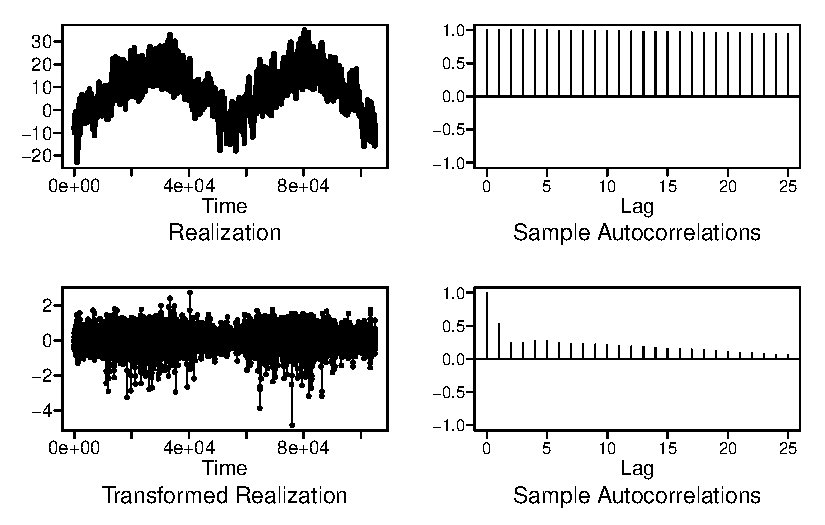
\includegraphics[keepaspectratio]{estudio_files/figure-pdf/unnamed-chunk-18-1.pdf}}

}

\caption{\label{fig-Temp_diferencias}Diferencias de los datos de
Temperatura (° F) en su serie temporal.}

\end{figure}%

En la Figura~\ref{fig-Temp_diferencias} se observa que después de
aplicar diferencias a los datos de Temperatura (° F) observamos que la
serie presenta estacionalidad.

\begin{Shaded}
\begin{Highlighting}[]
\CommentTok{\#library(tseries)}
\CommentTok{\#d2\_Temperatura = artrans.wge(d\_Temperatura,phi.tr= 1)}
\FunctionTok{kpss.test}\NormalTok{(d\_Temperatura, }\AttributeTok{null =} \StringTok{"Trend"}\NormalTok{)}
\end{Highlighting}
\end{Shaded}

\begin{verbatim}

    KPSS Test for Trend Stationarity

data:  d_Temperatura
KPSS Trend = 0.0026708, Truncation lag parameter = 22, p-value = 0.1
\end{verbatim}

Al aplicar la prueba KPSS a las diferencias a los datos de Temperatura
(°F) en su serie de tiempo, se obtiene un kpss estadístico menor
devuelto por el test, no se rechaza la hipótesis nula, confirmando la
estacionariedad en la serie de tiempo de la Temperatura (°F).

\subsubsection{Estandarización}\label{estandarizaciuxf3n-1}

Para que los datos sean comparables, es necesario estandarizarlos. Se
ajustan los datos históricos en su serie de tiempo para que su media sea
0 y su desviación estándar sea 1.

\begin{verbatim}
  [1] -1.555912e+00 -3.988778e-01  7.980539e-01  1.596903e-01  8.778494e-01
  [6]  1.715702e+00  9.944162e-05 -1.156935e+00 -2.074582e+00 -1.316525e+00
 [11] -4.786733e-01  1.197926e-01  7.989489e-02  6.783608e-01  9.944162e-05
 [16] -1.594915e-01 -4.387755e-01 -1.195937e-01 -3.988778e-01  9.944162e-05
 [21]  3.192812e-01 -5.185710e-01 -2.392869e-01 -7.180596e-01 -1.037241e+00
 [26] -3.979828e-02  5.985653e-01 -4.786733e-01 -6.382642e-01 -1.594915e-01
 [31] -3.979828e-02 -8.776505e-01 -3.979828e-02  1.596008e+00 -6.382642e-01
 [36]  3.192812e-01  1.755599e+00  9.576448e-01 -5.185710e-01 -1.555912e+00
 [41]  1.037440e+00  1.835395e+00  6.384630e-01  5.985653e-01  3.990767e-01
 [46]  6.783608e-01  1.197926e-01 -1.594915e-01  3.192812e-01  4.389744e-01
 [51]  8.379517e-01  6.783608e-01 -3.589801e-01 -1.993892e-01  5.985653e-01
 [56]  1.077338e+00  5.586676e-01  5.187699e-01 -7.969601e-02  3.999717e-02
 [61] -4.786733e-01 -4.387755e-01 -3.190824e-01 -3.979828e-02 -2.392869e-01
 [66] -2.791846e-01  3.990767e-01  6.783608e-01  1.995881e-01  5.187699e-01
 [71]  6.384630e-01  3.990767e-01  2.793835e-01  3.591790e-01  3.990767e-01
 [76]  1.197031e+00  1.276827e+00  2.394858e-01  2.793835e-01 -5.584687e-01
 [81] -2.791846e-01  3.591790e-01 -2.392869e-01  3.990767e-01  3.192812e-01
 [86]  3.999717e-02 -3.979828e-02  1.197926e-01  1.596903e-01  6.384630e-01
 [91] -1.594915e-01  5.586676e-01  4.389744e-01 -1.594915e-01 -1.594915e-01
 [96]  3.591790e-01  1.197926e-01 -1.594915e-01  1.197926e-01 -1.594915e-01
\end{verbatim}

\subsubsection{Normalización}\label{normalizaciuxf3n-1}

Esta transformación modifica la escala de los datos a un nuevo rango
entre 0 y 1.

\begin{verbatim}
  [1] 0.1326531 0.4285714 0.7346939 0.5714286 0.7551020 0.9693878 0.5306122
  [8] 0.2346939 0.0000000 0.1938776 0.4081633 0.5612245 0.5510204 0.7040816
 [15] 0.5306122 0.4897959 0.4183673 0.5000000 0.4285714 0.5306122 0.6122449
 [22] 0.3979592 0.4693878 0.3469388 0.2653061 0.5204082 0.6836735 0.4081633
 [29] 0.3673469 0.4897959 0.5204082 0.3061224 0.5204082 0.9387755 0.3673469
 [36] 0.6122449 0.9795918 0.7755102 0.3979592 0.1326531 0.7959184 1.0000000
 [43] 0.6938776 0.6836735 0.6326531 0.7040816 0.5612245 0.4897959 0.6122449
 [50] 0.6428571 0.7448980 0.7040816 0.4387755 0.4795918 0.6836735 0.8061224
 [57] 0.6734694 0.6632653 0.5102041 0.5408163 0.4081633 0.4183673 0.4489796
 [64] 0.5204082 0.4693878 0.4591837 0.6326531 0.7040816 0.5816327 0.6632653
 [71] 0.6938776 0.6326531 0.6020408 0.6224490 0.6326531 0.8367347 0.8571429
 [78] 0.5918367 0.6020408 0.3877551 0.4591837 0.6224490 0.4693878 0.6326531
 [85] 0.6122449 0.5408163 0.5204082 0.5612245 0.5714286 0.6938776 0.4897959
 [92] 0.6734694 0.6428571 0.4897959 0.4897959 0.6224490 0.5612245 0.4897959
 [99] 0.5612245 0.4897959
\end{verbatim}

Luego del ajuste preliminar de los datos históricos en su serie de
tiempo, se realizó una separación de los datos en dos grupos. Uno para
entrenamiento y otro para testeo.

\section{Implementación de la red neuronal
LSTM}\label{sec-implementaciuxf3n-de-la-red-neuronal-lstm}

En esta parte, se realizó el siguiente ajuste para su implementación en
lenguaje Python dentro del alterno \hyperref[sec-colab]{Colaboratory} de
los servicios gratuitos de google.

\subsection{Pronóstico mediante técnica
rodante}\label{pronuxf3stico-mediante-tuxe9cnica-rodante}

De las los 144 datos por día. En cada paso, se actualiza la secuencia de
entrada eliminando el valor más antiguo y agregando el último pronóstico
como el valor más reciente. Esto se ilustra esquemáticamente en la
Figura~\ref{fig-rodante}, donde \(n\) es la longitud rodante de la
secuencia de entrada y \(T\) es la longitud de la serie Temporal.

\begin{figure}

\centering{

\[
\begin{split}
y:\text{Observado}\quad &\quad \hat{y}:\text{Pronosticado}\\
y_{T-n+1}\quad y_{T-n+2}\quad y_{T-n+3}\quad&\cdots\quad y_{T-2}\quad y_{T-1}\quad y_T\quad \to\quad \color{orange}{\hat{y}_{T+1}}\\
y_{T-n+2}\quad y_{T-n+3}\quad y_{T-n+4}\quad&\cdots\quad y_{T-1}\quad y_{T}\quad \color{orange}{\hat{y}_{T+1}}\quad \to\quad \color{orange}{\hat{y}_{T+2}}\\
y_{T-n+3}\quad y_{T-n+4}\quad y_{T-n+5}\quad&\cdots\quad y_{T}\quad \color{orange}{\hat{y}_{T+1}}\quad \color{orange}{\hat{y}_{T+2}}\quad \to\quad \color{orange}{\hat{y}_{T+3}}\\
y_{T-n+4}\quad y_{T-n+5}\quad y_{T-n+6} \quad & \cdots\quad\color{orange}{\hat{y}_{T+1}}\quad\color{orange}{\hat{y}_{T+2}}\quad\color{orange}{\hat{y}_{T+3}}  \to\quad \color{orange}{\hat{y}_{T+4}}\\
&\ddots \\
\end{split}
\]

}

\caption{\label{fig-rodante}}

\end{figure}%

\subsection{Entrenamiento y calibración del modelo
LSTM}\label{entrenamiento-y-calibraciuxf3n-del-modelo-lstm}

Se procede al entrenamiento del modelo LSTM. La cantidad de capas
ocultas son 3. La primera capa LSTM, es una capas LSTM con 50 unidades
(neuronas). La segunda capa LSTM posee las mismas propiedades que la
capa anterior. Y la tercera capa, es una una capa densa de salida. El
tamaño del lote (batch size) es de 157, indica el número de muestras que
se usarán para actualizar los pesos del modelo en cada paso de
entrenamiento. Esta configuración se llevó a cabo con una función de
activación \hyperref[sec-Adam]{Adam}, ejecutando 100 iteraciones para el
entrenamiento de la red neuronal. La función de pérdida utilizada es el
error cuadrático medio (\hyperref[sec-MSE]{MSE}).

A continuación se exhibe el código utilizado.

\begin{Shaded}
\begin{Highlighting}[]
\CommentTok{\# univariate cnn example}
\ImportTok{import}\NormalTok{ numpy }\ImportTok{as}\NormalTok{ np}
\ImportTok{import}\NormalTok{ pandas }\ImportTok{as}\NormalTok{ pd}
\ImportTok{import}\NormalTok{ tensorflow }\ImportTok{as}\NormalTok{ tf}
\ImportTok{from}\NormalTok{ tensorflow.keras.layers }\ImportTok{import}\NormalTok{ Dense, LSTM}
\ImportTok{from}\NormalTok{ tensorflow.keras.models }\ImportTok{import}\NormalTok{ Sequential}
\ImportTok{from}\NormalTok{ sklearn.preprocessing }\ImportTok{import}\NormalTok{ MinMaxScaler}
\NormalTok{pd.options.mode.chained\_assignment }\OperatorTok{=} \VariableTok{None}
\NormalTok{tf.random.set\_seed(}\DecValTok{0}\NormalTok{)}



\ImportTok{from}\NormalTok{ google.colab }\ImportTok{import}\NormalTok{ drive}
\NormalTok{drive.mount(}\StringTok{\textquotesingle{}/content/drive\textquotesingle{}}\NormalTok{)}

\CommentTok{\# Leer set de datos}
\NormalTok{ruta }\OperatorTok{=} \StringTok{\textquotesingle{}/content/drive/My Drive/Colab Notebooks/\textquotesingle{}}
\NormalTok{df }\OperatorTok{=}\NormalTok{ pd.read\_csv(ruta}\OperatorTok{+}\StringTok{\textquotesingle{}datos\_clima\_wsu.csv\textquotesingle{}}\NormalTok{)}
\NormalTok{Times }\OperatorTok{=}\NormalTok{ df[}\StringTok{\textquotesingle{}Date Time\textquotesingle{}}\NormalTok{] }\CommentTok{\# Date}
\NormalTok{Temperatura }\OperatorTok{=}\NormalTok{ df[}\StringTok{\textquotesingle{}T(C°)\textquotesingle{}}\NormalTok{] }\CommentTok{\#Valiable}
\CommentTok{\#Tamaño de los Datos históricos}
\NormalTok{Temperatura }\OperatorTok{=}\NormalTok{ Temperatura[(}\DecValTok{7}\OperatorTok{*}\DecValTok{144}\NormalTok{):(}\DecValTok{22}\OperatorTok{*}\DecValTok{144}\NormalTok{)] }
\NormalTok{Temperatura }\OperatorTok{=}\NormalTok{ Temperatura }\OperatorTok{+} \FloatTok{273.15} 
\NormalTok{y }\OperatorTok{=}\NormalTok{ pd.DataFrame(\{}\StringTok{\textquotesingle{}Times\textquotesingle{}}\NormalTok{: Times, }\StringTok{\textquotesingle{}Temperatura\textquotesingle{}}\NormalTok{: Temperatura\})}
\CommentTok{\# Convertir la columna \textquotesingle{}fecha\textquotesingle{} al formato datetime de pandas}
\NormalTok{y[}\StringTok{\textquotesingle{}Times\textquotesingle{}}\NormalTok{] }\OperatorTok{=}\NormalTok{ pd.to\_datetime(y[}\StringTok{\textquotesingle{}Times\textquotesingle{}}\NormalTok{], }\BuiltInTok{format}\OperatorTok{=}\StringTok{\textquotesingle{}}\SpecialCharTok{\%d}\StringTok{.\%m.\%Y \%H:\%M:\%S\textquotesingle{}}\NormalTok{)}

\CommentTok{\# Establecer la columna \textquotesingle{}fecha\textquotesingle{} como el índice de la serie de tiempo}
\NormalTok{y.set\_index(}\StringTok{\textquotesingle{}Times\textquotesingle{}}\NormalTok{, inplace}\OperatorTok{=}\VariableTok{True}\NormalTok{)}
\NormalTok{y }\OperatorTok{=}\NormalTok{ y[}\StringTok{\textquotesingle{}Temperatura\textquotesingle{}}\NormalTok{].fillna(method}\OperatorTok{=}\StringTok{\textquotesingle{}ffill\textquotesingle{}}\NormalTok{)}
\NormalTok{y }\OperatorTok{=}\NormalTok{ y.values.reshape(}\OperatorTok{{-}}\DecValTok{1}\NormalTok{, }\DecValTok{1}\NormalTok{)}
\CommentTok{\# Escalamos los datos}
\NormalTok{scaler }\OperatorTok{=}\NormalTok{ MinMaxScaler(feature\_range}\OperatorTok{=}\NormalTok{(}\DecValTok{0}\NormalTok{, }\DecValTok{1}\NormalTok{))}
\NormalTok{scaler }\OperatorTok{=}\NormalTok{ scaler.fit(y)}
\NormalTok{y }\OperatorTok{=}\NormalTok{ scaler.transform(y)}
\end{Highlighting}
\end{Shaded}

\begin{Shaded}
\begin{Highlighting}[]
\CommentTok{\# CNN para datos univariados }
\ImportTok{import}\NormalTok{ numpy }\ImportTok{as}\NormalTok{ np}
\ImportTok{import}\NormalTok{ pandas }\ImportTok{as}\NormalTok{ pd}
\ImportTok{import}\NormalTok{ tensorflow }\ImportTok{as}\NormalTok{ tf}
\ImportTok{from}\NormalTok{ tensorflow.keras.layers }\ImportTok{import}\NormalTok{ Dense, LSTM}
\ImportTok{from}\NormalTok{ tensorflow.keras.models }\ImportTok{import}\NormalTok{ Sequential}
\ImportTok{from}\NormalTok{ sklearn.preprocessing }\ImportTok{import}\NormalTok{ MinMaxScaler}
\NormalTok{pd.options.mode.chained\_assignment }\OperatorTok{=} \VariableTok{None}
\NormalTok{tf.random.set\_seed(}\DecValTok{0}\NormalTok{)}

\ImportTok{import}\NormalTok{ matplotlib.pyplot }\ImportTok{as}\NormalTok{ plt}

\CommentTok{\# Grafica el Loss}
\KeywordTok{def}\NormalTok{ train\_and\_plot\_loss(model, X, y, epochs}\OperatorTok{=}\DecValTok{100}\NormalTok{, verbose}\OperatorTok{=}\DecValTok{2}\NormalTok{):}
\NormalTok{    history }\OperatorTok{=}\NormalTok{ model.fit(X, Y, epochs}\OperatorTok{=}\DecValTok{100}\NormalTok{, }
\NormalTok{    batch\_size}\OperatorTok{=}\DecValTok{314}\NormalTok{, verbose}\OperatorTok{=}\DecValTok{2}\NormalTok{, shuffle}\OperatorTok{=}\VariableTok{False}\NormalTok{)}


    \CommentTok{\# Graficar el loss}
\NormalTok{    plt.plot(history.history[}\StringTok{\textquotesingle{}loss\textquotesingle{}}\NormalTok{])}
\NormalTok{    plt.title(}\StringTok{\textquotesingle{}Model Loss\textquotesingle{}}\NormalTok{)}
\NormalTok{    plt.xlabel(}\StringTok{\textquotesingle{}Epoch\textquotesingle{}}\NormalTok{)}
\NormalTok{    plt.ylabel(}\StringTok{\textquotesingle{}Loss\textquotesingle{}}\NormalTok{)}
\NormalTok{    plt.show()}

\ImportTok{from}\NormalTok{ google.colab }\ImportTok{import}\NormalTok{ drive}
\NormalTok{drive.mount(}\StringTok{\textquotesingle{}/content/drive\textquotesingle{}}\NormalTok{)}

\CommentTok{\# Leer set de datos}
\NormalTok{ruta }\OperatorTok{=} \StringTok{\textquotesingle{}/content/drive/My Drive/Colab Notebooks/\textquotesingle{}}
\NormalTok{df }\OperatorTok{=}\NormalTok{ pd.read\_csv(ruta}\OperatorTok{+}\StringTok{\textquotesingle{}datos\_clima\_wsu.csv\textquotesingle{}}\NormalTok{)}
\NormalTok{Times }\OperatorTok{=}\NormalTok{ df[}\StringTok{\textquotesingle{}Date Time\textquotesingle{}}\NormalTok{] }\CommentTok{\# Date}
\NormalTok{Temperatura }\OperatorTok{=}\NormalTok{ df[}\StringTok{\textquotesingle{}T(C°)\textquotesingle{}}\NormalTok{] }\CommentTok{\#Valiable}
\CommentTok{\#Tamaño de los Datos historicos}
\NormalTok{Temperatura }\OperatorTok{=}\NormalTok{ Temperatura[(}\DecValTok{7}\OperatorTok{*}\DecValTok{144}\NormalTok{):(}\DecValTok{22}\OperatorTok{*}\DecValTok{144}\NormalTok{)] }
\NormalTok{Temperatura }\OperatorTok{=}\NormalTok{ Temperatura }\OperatorTok{+} \FloatTok{273.15} 
\NormalTok{y }\OperatorTok{=}\NormalTok{ pd.DataFrame(\{}\StringTok{\textquotesingle{}Times\textquotesingle{}}\NormalTok{: Times, }\StringTok{\textquotesingle{}Temperatura\textquotesingle{}}\NormalTok{: Temperatura\})}
\CommentTok{\# Convertir la columna \textquotesingle{}fecha\textquotesingle{} al formato datetime de pandas}
\NormalTok{y[}\StringTok{\textquotesingle{}Times\textquotesingle{}}\NormalTok{] }\OperatorTok{=}\NormalTok{ pd.to\_datetime(y[}\StringTok{\textquotesingle{}Times\textquotesingle{}}\NormalTok{], }\BuiltInTok{format}\OperatorTok{=}\StringTok{\textquotesingle{}}\SpecialCharTok{\%d}\StringTok{.\%m.\%Y \%H:\%M:\%S\textquotesingle{}}\NormalTok{)}

\CommentTok{\# Establecer la columna \textquotesingle{}fecha\textquotesingle{} como el índice de la serie de tiempo}
\NormalTok{y.set\_index(}\StringTok{\textquotesingle{}Times\textquotesingle{}}\NormalTok{, inplace}\OperatorTok{=}\VariableTok{True}\NormalTok{)}
\NormalTok{y }\OperatorTok{=}\NormalTok{ y[}\StringTok{\textquotesingle{}Temperatura\textquotesingle{}}\NormalTok{].fillna(method}\OperatorTok{=}\StringTok{\textquotesingle{}ffill\textquotesingle{}}\NormalTok{)}
\NormalTok{y }\OperatorTok{=}\NormalTok{ y.values.reshape(}\OperatorTok{{-}}\DecValTok{1}\NormalTok{, }\DecValTok{1}\NormalTok{)}
\CommentTok{\# Escalamiento de  los datos}
\NormalTok{scaler }\OperatorTok{=}\NormalTok{ MinMaxScaler(feature\_range}\OperatorTok{=}\NormalTok{(}\DecValTok{0}\NormalTok{, }\DecValTok{1}\NormalTok{))}
\NormalTok{scaler }\OperatorTok{=}\NormalTok{ scaler.fit(y)}
\NormalTok{y }\OperatorTok{=}\NormalTok{ scaler.transform(y)}

\CommentTok{\# generar las secuencias de entrada y salida}
\NormalTok{n\_lookback }\OperatorTok{=} \DecValTok{6}\OperatorTok{*}\DecValTok{144}  \CommentTok{\#Secuancia de entrada}
\CommentTok{\# Secuancia de salida (o Número de predicciones)}
\NormalTok{n\_forecast }\OperatorTok{=} \DecValTok{144}\OperatorTok{*}\DecValTok{4} 

\CommentTok{\# Inicializar DataFrame para almacenar los resultados}
\NormalTok{resultados\_df }\OperatorTok{=}\NormalTok{ pd.DataFrame()}
\NormalTok{k }\OperatorTok{=} \DecValTok{50}
\CommentTok{\# Genera (k) simulaciones de la predicción}
\ControlFlowTok{for}\NormalTok{ repeticion }\KeywordTok{in} \BuiltInTok{range}\NormalTok{(k):}
\NormalTok{    X }\OperatorTok{=}\NormalTok{ []}
\NormalTok{    Y }\OperatorTok{=}\NormalTok{ []}

    \ControlFlowTok{for}\NormalTok{ i }\KeywordTok{in} \BuiltInTok{range}\NormalTok{(n\_lookback, }\BuiltInTok{len}\NormalTok{(y) }\OperatorTok{{-}}\NormalTok{ n\_forecast }\OperatorTok{+} \DecValTok{1}\NormalTok{):}
\NormalTok{        X.append(y[i }\OperatorTok{{-}}\NormalTok{ n\_lookback: i])}
\NormalTok{        Y.append(y[i: i }\OperatorTok{+}\NormalTok{ n\_forecast])}

\NormalTok{    X }\OperatorTok{=}\NormalTok{ np.array(X)}
\NormalTok{    Y }\OperatorTok{=}\NormalTok{ np.array(Y)}

    \CommentTok{\# Crea el modelo}
\NormalTok{    model }\OperatorTok{=}\NormalTok{ Sequential()}
\NormalTok{    model.add(LSTM(units}\OperatorTok{=}\DecValTok{50}\NormalTok{, return\_sequences}\OperatorTok{=}\VariableTok{True}\NormalTok{,}
\NormalTok{              input\_shape}\OperatorTok{=}\NormalTok{(n\_lookback, }\DecValTok{1}\NormalTok{)))}
\NormalTok{    model.add(LSTM(units}\OperatorTok{=}\DecValTok{50}\NormalTok{))}
\NormalTok{    model.add(Dense(n\_forecast))}
\NormalTok{    model.}\BuiltInTok{compile}\NormalTok{(loss}\OperatorTok{=}\StringTok{\textquotesingle{}mean\_squared\_error\textquotesingle{}}\NormalTok{, optimizer}\OperatorTok{=}\StringTok{\textquotesingle{}adam\textquotesingle{}}\NormalTok{)}
    \CommentTok{\#Entrenamiento del modelo}
\NormalTok{    train\_and\_plot\_loss(model, X, y, epochs}\OperatorTok{=}\DecValTok{100}\NormalTok{, verbose}\OperatorTok{=}\DecValTok{2}\NormalTok{)}
    

    \CommentTok{\# Genera los pronósticos}
\NormalTok{    X\_ }\OperatorTok{=}\NormalTok{ y[}\OperatorTok{{-}}\NormalTok{n\_lookback:]}
\NormalTok{    X\_ }\OperatorTok{=}\NormalTok{ X\_.reshape(}\DecValTok{1}\NormalTok{, n\_lookback, }\DecValTok{1}\NormalTok{)}

\NormalTok{    Y\_ }\OperatorTok{=}\NormalTok{ model.predict(X\_).reshape(}\OperatorTok{{-}}\DecValTok{1}\NormalTok{, }\DecValTok{1}\NormalTok{)}
\NormalTok{    Y\_ }\OperatorTok{=}\NormalTok{ scaler.inverse\_transform(Y\_)}

    \CommentTok{\# Agregar resultados al DataFrame}
\NormalTok{    resultados\_df[}\SpecialStringTok{f\textquotesingle{}Repeticion\_}\SpecialCharTok{\{}\NormalTok{repeticion }\OperatorTok{+} \DecValTok{1}\SpecialCharTok{\}}\SpecialStringTok{\textquotesingle{}}\NormalTok{] }\OperatorTok{=}\NormalTok{ Y\_.flatten()}

\CommentTok{\# Mostrar el DataFrame con los resultados}
\BuiltInTok{print}\NormalTok{(resultados\_df)}
\end{Highlighting}
\end{Shaded}

\begin{figure}

\centering{

\pandocbounded{\includegraphics[keepaspectratio]{LOSS_LSTM.png}}

}

\caption{\label{fig-loss_LSTM}Gráfica de la función de pérdida para la
red neuronal LSTM}

\end{figure}%

En la Figura~\ref{fig-loss_LSTM} se observa la trayectoria del valor de
la \hyperref[sec-funciuxf3n-de-perdida]{función de pérdida} en cada
época del entrenamiento en la red neuronal LSTM.

\section{Implementación de la red neuronal convolucional
(CNN)}\label{sec-implementaciuxf3n-de-la-red-neuronal-cnn.}

En esta parte, se realizó el mismo ajuste que en la red neuronal LSTM
para su implementación en Python dentro de un servidor gratuito de
\hyperref[sec-colab]{Colaboratory}.

Se procede al entrenamiento de la red neuronal convolucional (CNN). La
cantidad de capas ocultas son 5 capas, de las cuales, la primera capa es
una capa es convolucional unidimensional, donde va aprender a través de
64 mapas de características y con un tamaño de
\hyperref[sec-kernel]{kernel} de dimensión 5. La segunda capa es una
Capa \hyperref[sec-pooling]{Max-pooling} unidimensional, la tercera capa
es una capa de aplanar (\hyperref[sec-fratten]{flatten}), la cuarta capa
es una capa Densa, la quinta capa es Densa (salida). Asimismo, se eligió
la función de activación \hyperref[sec-Relu]{ReLu}, y el proceso de
entrenamiento del modelo se ejecutó a lo largo de 25 iteraciones, 70
iteraciones y 100 iteraciones según los datos históricos.

A continuación se exhibe el código utilizado.

\begin{Shaded}
\begin{Highlighting}[]
\CommentTok{\# univariate cnn example}
\ImportTok{from}\NormalTok{ numpy }\ImportTok{import}\NormalTok{ array}
\ImportTok{from}\NormalTok{ keras.models }\ImportTok{import}\NormalTok{ Sequential}
\ImportTok{from}\NormalTok{ keras.layers }\ImportTok{import}\NormalTok{ Dense}
\ImportTok{from}\NormalTok{ keras.layers }\ImportTok{import}\NormalTok{ Flatten}
\ImportTok{from}\NormalTok{ tensorflow.keras.models }\ImportTok{import}\NormalTok{ Sequential}
\ImportTok{from}\NormalTok{ tensorflow.keras.layers }\ImportTok{import}\NormalTok{ Conv1D, MaxPooling1D, Flatten, Dense}
\ImportTok{from}\NormalTok{ tensorflow.keras.optimizers }\ImportTok{import}\NormalTok{ RMSprop}
\ImportTok{import}\NormalTok{ matplotlib.pyplot }\ImportTok{as}\NormalTok{ plt}
\ImportTok{from}\NormalTok{ keras }\ImportTok{import}\NormalTok{ backend }\ImportTok{as}\NormalTok{ K}

\ImportTok{import}\NormalTok{ numpy }\ImportTok{as}\NormalTok{ np}
\ImportTok{import}\NormalTok{ pandas }\ImportTok{as}\NormalTok{ pd}
\ImportTok{import}\NormalTok{ yfinance }\ImportTok{as}\NormalTok{ yf}
\ImportTok{import}\NormalTok{ tensorflow }\ImportTok{as}\NormalTok{ tf}
\ImportTok{from}\NormalTok{ tensorflow.keras.layers }\ImportTok{import}\NormalTok{ Dense, LSTM}
\ImportTok{from}\NormalTok{ tensorflow.keras.models }\ImportTok{import}\NormalTok{ Sequential}
\ImportTok{from}\NormalTok{ sklearn.preprocessing }\ImportTok{import}\NormalTok{ MinMaxScaler }


\CommentTok{\# split a univariate sequence into samples}
\KeywordTok{def}\NormalTok{ split\_sequence(sequence, n\_steps):}
\NormalTok{    X, y }\OperatorTok{=} \BuiltInTok{list}\NormalTok{(), }\BuiltInTok{list}\NormalTok{()}
    \ControlFlowTok{for}\NormalTok{ i }\KeywordTok{in} \BuiltInTok{range}\NormalTok{(}\BuiltInTok{len}\NormalTok{(sequence)):}
        \CommentTok{\# find the end of this pattern}
\NormalTok{        end\_ix }\OperatorTok{=}\NormalTok{ i }\OperatorTok{+}\NormalTok{ n\_steps}
        \CommentTok{\# check if we are beyond the sequence}
        \ControlFlowTok{if}\NormalTok{ end\_ix }\OperatorTok{\textgreater{}} \BuiltInTok{len}\NormalTok{(sequence)}\OperatorTok{{-}}\DecValTok{1}\NormalTok{:}
            \ControlFlowTok{break}
        \CommentTok{\# gather input and output parts of the pattern}
\NormalTok{        seq\_x, seq\_y }\OperatorTok{=}\NormalTok{ sequence[i:end\_ix], sequence[end\_ix]}
\NormalTok{        X.append(seq\_x)}
\NormalTok{        y.append(seq\_y)}
    \ControlFlowTok{return}\NormalTok{ array(X), array(y)}


\KeywordTok{def}\NormalTok{ train\_and\_plot\_loss(model, X, y, epochs}\OperatorTok{=}\DecValTok{20}\NormalTok{, verbose}\OperatorTok{=}\DecValTok{1}\NormalTok{):}
\NormalTok{    history }\OperatorTok{=}\NormalTok{ model.fit(X, y, epochs}\OperatorTok{=}\NormalTok{epochs, verbose}\OperatorTok{=}\NormalTok{verbose)}
    \CommentTok{\# Graficar el loss}
\NormalTok{    plt.plot(history.history[}\StringTok{\textquotesingle{}loss\textquotesingle{}}\NormalTok{])}
\NormalTok{    plt.title(}\StringTok{\textquotesingle{}Model Loss\textquotesingle{}}\NormalTok{)}
\NormalTok{    plt.xlabel(}\StringTok{\textquotesingle{}Epoch\textquotesingle{}}\NormalTok{)}
\NormalTok{    plt.ylabel(}\StringTok{\textquotesingle{}Loss\textquotesingle{}}\NormalTok{)}
\NormalTok{    plt.show()}

    
    
\ImportTok{from}\NormalTok{ google.colab }\ImportTok{import}\NormalTok{ drive}
\NormalTok{drive.mount(}\StringTok{\textquotesingle{}/content/drive\textquotesingle{}}\NormalTok{)}


\CommentTok{\# Leer set de datos}
\NormalTok{ruta }\OperatorTok{=} \StringTok{\textquotesingle{}/content/drive/My Drive/Colab Notebooks/\textquotesingle{}}
\NormalTok{df }\OperatorTok{=}\NormalTok{ pd.read\_csv(ruta}\OperatorTok{+}\StringTok{\textquotesingle{}datos\_clima\_wsu.csv\textquotesingle{}}\NormalTok{)}

\NormalTok{Temperatura }\OperatorTok{=}\NormalTok{ df[}\StringTok{\textquotesingle{}T(C°)\textquotesingle{}}\NormalTok{] }\CommentTok{\#Valiable}
\CommentTok{\#Tamaño de los Datos historicos}
\NormalTok{Temperatura }\OperatorTok{=}\NormalTok{ Temperatura[(}\DecValTok{7}\OperatorTok{*}\DecValTok{144}\NormalTok{):(}\DecValTok{37}\OperatorTok{*}\DecValTok{144}\NormalTok{)] }
\NormalTok{Temperatura }\OperatorTok{=}\NormalTok{ Temperatura }\OperatorTok{+} \FloatTok{273.15} 

\CommentTok{\# Escalar los datos entre 0 y 1}
\NormalTok{scaler }\OperatorTok{=}\NormalTok{ MinMaxScaler(feature\_range}\OperatorTok{=}\NormalTok{(}\DecValTok{0}\NormalTok{, }\DecValTok{1}\NormalTok{))}
\NormalTok{Datos\_historicos }\OperatorTok{=}\NormalTok{ scaler.fit\_transform(Temperatura.values.reshape(}\OperatorTok{{-}}\DecValTok{1}\NormalTok{, }\DecValTok{1}\NormalTok{))}
\end{Highlighting}
\end{Shaded}

\begin{Shaded}
\begin{Highlighting}[]
\CommentTok{\# univariate cnn example}
\ImportTok{from}\NormalTok{ numpy }\ImportTok{import}\NormalTok{ array}
\ImportTok{from}\NormalTok{ keras.models }\ImportTok{import}\NormalTok{ Sequential}
\ImportTok{from}\NormalTok{ keras.layers }\ImportTok{import}\NormalTok{ Dense}
\ImportTok{from}\NormalTok{ keras.layers }\ImportTok{import}\NormalTok{ Flatten}
\ImportTok{from}\NormalTok{ tensorflow.keras.models }\ImportTok{import}\NormalTok{ Sequential}
\ImportTok{from}\NormalTok{ tensorflow.keras.layers }\ImportTok{import}\NormalTok{ Conv1D, MaxPooling1D, Flatten, Dense}
\ImportTok{from}\NormalTok{ tensorflow.keras.optimizers }\ImportTok{import}\NormalTok{ RMSprop}
\ImportTok{import}\NormalTok{ matplotlib.pyplot }\ImportTok{as}\NormalTok{ plt}
\ImportTok{from}\NormalTok{ keras }\ImportTok{import}\NormalTok{ backend }\ImportTok{as}\NormalTok{ K}

\ImportTok{import}\NormalTok{ numpy }\ImportTok{as}\NormalTok{ np}
\ImportTok{import}\NormalTok{ pandas }\ImportTok{as}\NormalTok{ pd}
\ImportTok{import}\NormalTok{ tensorflow }\ImportTok{as}\NormalTok{ tf}
\ImportTok{from}\NormalTok{ tensorflow.keras.layers }\ImportTok{import}\NormalTok{ Dense, LSTM}
\ImportTok{from}\NormalTok{ tensorflow.keras.models }\ImportTok{import}\NormalTok{ Sequential}
\ImportTok{from}\NormalTok{ sklearn.preprocessing }\ImportTok{import}\NormalTok{ MinMaxScaler    }


\CommentTok{\#Divide una secuencia univariada en muestras}
\KeywordTok{def}\NormalTok{ split\_sequence(sequence, n\_steps):}
\NormalTok{    X, y }\OperatorTok{=} \BuiltInTok{list}\NormalTok{(), }\BuiltInTok{list}\NormalTok{()}
    \ControlFlowTok{for}\NormalTok{ i }\KeywordTok{in} \BuiltInTok{range}\NormalTok{(}\BuiltInTok{len}\NormalTok{(sequence)):}
        \CommentTok{\# Encuentra el final de este patrón}
\NormalTok{        end\_ix }\OperatorTok{=}\NormalTok{ i }\OperatorTok{+}\NormalTok{ n\_steps}
        \CommentTok{\#Comprueba si se está más allá de la secuencia}
        \ControlFlowTok{if}\NormalTok{ end\_ix }\OperatorTok{\textgreater{}} \BuiltInTok{len}\NormalTok{(sequence)}\OperatorTok{{-}}\DecValTok{1}\NormalTok{:}
            \ControlFlowTok{break}
        \CommentTok{\#Reune las partes de entrada y salida del patrón}
\NormalTok{        seq\_x, seq\_y }\OperatorTok{=}\NormalTok{ sequence[i:end\_ix], sequence[end\_ix]}
\NormalTok{        X.append(seq\_x)}
\NormalTok{        y.append(seq\_y)}
    \ControlFlowTok{return}\NormalTok{ array(X), array(y)}

\KeywordTok{def}\NormalTok{ train\_and\_plot\_loss(model, X, y, epochs}\OperatorTok{=}\DecValTok{20}\NormalTok{, verbose}\OperatorTok{=}\DecValTok{1}\NormalTok{):}
\NormalTok{    history }\OperatorTok{=}\NormalTok{ model.fit(X, y, epochs}\OperatorTok{=}\NormalTok{epochs, verbose}\OperatorTok{=}\NormalTok{verbose)}
    \CommentTok{\# Graficar el loss}
\NormalTok{    plt.plot(history.history[}\StringTok{\textquotesingle{}loss\textquotesingle{}}\NormalTok{])}
\NormalTok{    plt.title(}\StringTok{\textquotesingle{}Model Loss\textquotesingle{}}\NormalTok{)}
\NormalTok{    plt.xlabel(}\StringTok{\textquotesingle{}Epoch\textquotesingle{}}\NormalTok{)}
\NormalTok{    plt.ylabel(}\StringTok{\textquotesingle{}Loss\textquotesingle{}}\NormalTok{)}
\NormalTok{    plt.show()}

    
\CommentTok{\#Ubica el Drive del archivo    }
\ImportTok{from}\NormalTok{ google.colab }\ImportTok{import}\NormalTok{ drive}
\NormalTok{drive.mount(}\StringTok{\textquotesingle{}/content/drive\textquotesingle{}}\NormalTok{)}


\CommentTok{\# Leer set de datos}
\NormalTok{ruta }\OperatorTok{=} \StringTok{\textquotesingle{}/content/drive/My Drive/Colab Notebooks/\textquotesingle{}}
\NormalTok{df }\OperatorTok{=}\NormalTok{ pd.read\_csv(ruta}\OperatorTok{+}\StringTok{\textquotesingle{}datos\_clima\_wsu.csv\textquotesingle{}}\NormalTok{)}
\NormalTok{Temperatura }\OperatorTok{=}\NormalTok{ df[}\StringTok{\textquotesingle{}T(C°)\textquotesingle{}}\NormalTok{] }\CommentTok{\#Valiable}
\CommentTok{\#Tamaño de los Datos históricos}
\NormalTok{Temperatura }\OperatorTok{=}\NormalTok{ Temperatura[(}\DecValTok{7}\OperatorTok{*}\DecValTok{144}\NormalTok{):(}\DecValTok{37}\OperatorTok{*}\DecValTok{144}\NormalTok{)] }
\NormalTok{Temperatura }\OperatorTok{=}\NormalTok{ Temperatura }\OperatorTok{+} \FloatTok{273.15} 

\CommentTok{\# Se escalan los datos entre 0 y 1}
\NormalTok{scaler }\OperatorTok{=}\NormalTok{ MinMaxScaler(feature\_range}\OperatorTok{=}\NormalTok{(}\DecValTok{0}\NormalTok{, }\DecValTok{1}\NormalTok{))}
\NormalTok{Datos\_historicos }\OperatorTok{=}\NormalTok{ scaler.fit\_transform(Temperatura.values.reshape(}\OperatorTok{{-}}\DecValTok{1}\NormalTok{, }\DecValTok{1}\NormalTok{))}
\end{Highlighting}
\end{Shaded}

\begin{Shaded}
\begin{Highlighting}[]
\CommentTok{\#Define la secuencia de entrada}
\NormalTok{raw\_seq }\OperatorTok{=}\NormalTok{ Datos\_historicos  }
\CommentTok{\# Cantidad de pasos de tiempo}
\NormalTok{n\_steps }\OperatorTok{=} \DecValTok{144}
\CommentTok{\# se divide las muestras}
\NormalTok{X, y }\OperatorTok{=}\NormalTok{ split\_sequence(raw\_seq, n\_steps)}
\NormalTok{n\_features }\OperatorTok{=} \DecValTok{1}
\CommentTok{\#[muestras, pasos de tiempo, características]}
\NormalTok{X }\OperatorTok{=}\NormalTok{ X.reshape((X.shape[}\DecValTok{0}\NormalTok{],X.shape[}\DecValTok{1}\NormalTok{], n\_features))  }
\CommentTok{\# Crear un modelo secuencial}
\NormalTok{model }\OperatorTok{=}\NormalTok{ Sequential()}
\NormalTok{model.add(Conv1D(}\DecValTok{64}\NormalTok{, kernel\_size}\OperatorTok{=}\DecValTok{5}\NormalTok{, }
\NormalTok{  activation}\OperatorTok{=}\StringTok{\textquotesingle{}relu\textquotesingle{}}\NormalTok{,input\_shape}\OperatorTok{=}\NormalTok{(n\_steps, n\_features)))}
\NormalTok{model.add(MaxPooling1D(pool\_size}\OperatorTok{=}\DecValTok{5}\NormalTok{))}
\NormalTok{model.add(Flatten())}
\NormalTok{model.add(Dense(}\DecValTok{50}\NormalTok{, activation}\OperatorTok{=}\StringTok{\textquotesingle{}relu\textquotesingle{}}\NormalTok{))}
\NormalTok{model.add(Dense(}\DecValTok{1}\NormalTok{))}
\NormalTok{model.}\BuiltInTok{compile}\NormalTok{(optimizer}\OperatorTok{=}\NormalTok{RMSprop(clipvalue}\OperatorTok{=}\FloatTok{1.0}\NormalTok{), loss}\OperatorTok{=}\StringTok{\textquotesingle{}mae\textquotesingle{}}\NormalTok{)}
\CommentTok{\# Entreniento}
\NormalTok{train\_and\_plot\_loss(model, X, y, epochs}\OperatorTok{=}\DecValTok{100}\NormalTok{, verbose}\OperatorTok{=}\DecValTok{1}\NormalTok{)}
\end{Highlighting}
\end{Shaded}

\begin{figure}

\centering{

\pandocbounded{\includegraphics[keepaspectratio]{loss_convolucional.png}}

}

\caption{\label{fig-loss_cnn}Gráfica de la función de pérdida obtenida
mediante una CNN con el conjunto de datos históricos de la variable
Temperatura (°F).}

\end{figure}%

En la Figura~\ref{fig-loss_cnn} se muestra la variación del valor de la
\hyperref[sec-funciuxf3n-de-perdida]{función de pérdida} a lo largo del
entrenamiento de la red neuronal convolucional (CNN).

\begin{Shaded}
\begin{Highlighting}[]
\NormalTok{num\_simulaciones }\OperatorTok{=} \DecValTok{50}
\NormalTok{simulaciones\_df }\OperatorTok{=}\NormalTok{ pd.DataFrame()}

\NormalTok{prediccion }\OperatorTok{=}\NormalTok{ []}
\CommentTok{\# Preparación de datos de entrada para la predicción}
\NormalTok{x\_input }\OperatorTok{=}\NormalTok{ y[(}\DecValTok{144}\OperatorTok{*}\DecValTok{28}\NormalTok{):(}\DecValTok{144}\OperatorTok{*}\DecValTok{29}\NormalTok{)]}
\NormalTok{n }\OperatorTok{=} \BuiltInTok{len}\NormalTok{(x\_input)}
\NormalTok{n\_steps }\OperatorTok{=} \DecValTok{144}
\NormalTok{n\_features }\OperatorTok{=} \DecValTok{1}
\NormalTok{x\_input }\OperatorTok{=}\NormalTok{  x\_input.reshape((}\DecValTok{1}\NormalTok{, n\_steps, n\_features))}

\CommentTok{\# Predicción con el modelo entrenado}
\NormalTok{yhat }\OperatorTok{=}\NormalTok{ model.predict(x\_input, verbose}\OperatorTok{=}\DecValTok{0}\NormalTok{).reshape(}\OperatorTok{{-}}\DecValTok{1}\NormalTok{,}\DecValTok{1}\NormalTok{)}
\NormalTok{aux}\OperatorTok{=}\NormalTok{ yhat}
\NormalTok{aux }\OperatorTok{=}\NormalTok{ scaler.inverse\_transform(aux)}


\ControlFlowTok{for}\NormalTok{ sim }\KeywordTok{in} \BuiltInTok{range}\NormalTok{(num\_simulaciones):}
\NormalTok{    k }\OperatorTok{=} \DecValTok{144}\OperatorTok{*}\DecValTok{4}
\NormalTok{    prediccion }\OperatorTok{=}\NormalTok{ []}
\NormalTok{    i }\OperatorTok{=} \DecValTok{0}
    \ControlFlowTok{for}\NormalTok{ \_ }\KeywordTok{in} \BuiltInTok{range}\NormalTok{(k):}
\NormalTok{        x\_new }\OperatorTok{=}\NormalTok{ yhat[}\OperatorTok{{-}}\NormalTok{n\_steps:]}
\NormalTok{        x\_input }\OperatorTok{=}\NormalTok{ np.append(x\_input, x\_new)}
\NormalTok{        x\_input }\OperatorTok{=}\NormalTok{ x\_input[}\OperatorTok{{-}}\NormalTok{n\_steps:]}
\NormalTok{        x\_input }\OperatorTok{=}\NormalTok{ x\_input.reshape((}\DecValTok{1}\NormalTok{, }\BuiltInTok{len}\NormalTok{(x\_input), n\_features))}
\NormalTok{        yhat }\OperatorTok{=}\NormalTok{ model.predict(x\_input, verbose}\OperatorTok{=}\DecValTok{0}\NormalTok{).reshape(}\OperatorTok{{-}}\DecValTok{1}\NormalTok{,}\DecValTok{1}\NormalTok{)}
\NormalTok{        aux}\OperatorTok{=}\NormalTok{ yhat}
\NormalTok{        aux }\OperatorTok{=}\NormalTok{ scaler.inverse\_transform(aux)}
\NormalTok{        prediccion.append(aux)}
        \BuiltInTok{print}\NormalTok{(}\StringTok{"Pronóstico para los próximos"}\NormalTok{, i, }\StringTok{"valores:"}\NormalTok{, aux)}
\NormalTok{        i}\OperatorTok{+=} \DecValTok{1}
    \CommentTok{\# Agregar los resultados de la simulación actual al DataFrame}
\NormalTok{    simulaciones\_df[}\SpecialStringTok{f\textquotesingle{}Simulacion\_}\SpecialCharTok{\{}\NormalTok{sim}\OperatorTok{+}\DecValTok{1}\SpecialCharTok{\}}\SpecialStringTok{\textquotesingle{}}\NormalTok{] }\OperatorTok{=}\NormalTok{ prediccion}
    \KeywordTok{del}\NormalTok{ model}
\NormalTok{    raw\_seq }\OperatorTok{=}\NormalTok{ Datos\_historicos}
\NormalTok{    n\_steps }\OperatorTok{=} \DecValTok{144}
\NormalTok{    X, y }\OperatorTok{=}\NormalTok{ split\_sequence(raw\_seq, n\_steps)}
\NormalTok{    n\_features }\OperatorTok{=} \DecValTok{1}
\NormalTok{    X }\OperatorTok{=}\NormalTok{ X.reshape((X.shape[}\DecValTok{0}\NormalTok{],X.shape[}\DecValTok{1}\NormalTok{], n\_features))}

\NormalTok{    model }\OperatorTok{=}\NormalTok{ Sequential()}
\NormalTok{    model.add(Conv1D(}\DecValTok{64}\NormalTok{, kernel\_size}\OperatorTok{=}\DecValTok{5}\NormalTok{, activation}\OperatorTok{=}\StringTok{\textquotesingle{}relu\textquotesingle{}}\NormalTok{, }
\NormalTok{    input\_shape}\OperatorTok{=}\NormalTok{(n\_steps, n\_features)))}
\NormalTok{    model.add(MaxPooling1D(pool\_size}\OperatorTok{=}\DecValTok{5}\NormalTok{))}
\NormalTok{    model.add(Flatten())}
\NormalTok{    model.add(Dense(}\DecValTok{50}\NormalTok{, activation}\OperatorTok{=}\StringTok{\textquotesingle{}relu\textquotesingle{}}\NormalTok{))}
\NormalTok{    model.add(Dense(}\DecValTok{1}\NormalTok{))}
\NormalTok{    model.}\BuiltInTok{compile}\NormalTok{(optimizer}\OperatorTok{=}\NormalTok{RMSprop(clipvalue}\OperatorTok{=}\FloatTok{1.0}\NormalTok{), loss}\OperatorTok{=}\StringTok{\textquotesingle{}mae\textquotesingle{}}\NormalTok{)}
    \CommentTok{\# Entrenamiento del modelo}
\NormalTok{    model.fit(X, y, epochs}\OperatorTok{=}\DecValTok{100}\NormalTok{, verbose}\OperatorTok{=}\DecValTok{1}\NormalTok{)}
\NormalTok{    x\_input }\OperatorTok{=}\NormalTok{ y[(}\DecValTok{144}\OperatorTok{*}\DecValTok{28}\NormalTok{):(}\DecValTok{144}\OperatorTok{*}\DecValTok{29}\NormalTok{)]}
\NormalTok{    n }\OperatorTok{=} \BuiltInTok{len}\NormalTok{(x\_input)}
\NormalTok{    n\_steps }\OperatorTok{=} \DecValTok{144}
\NormalTok{    n\_features }\OperatorTok{=} \DecValTok{1}
\NormalTok{    x\_input }\OperatorTok{=}\NormalTok{  x\_input.reshape((}\DecValTok{1}\NormalTok{, n\_steps, n\_features))}
    \CommentTok{\# Predicción con el modelo entrenado}
\NormalTok{    yhat }\OperatorTok{=}\NormalTok{ model.predict(x\_input, verbose}\OperatorTok{=}\DecValTok{0}\NormalTok{).reshape(}\OperatorTok{{-}}\DecValTok{1}\NormalTok{, }\DecValTok{1}\NormalTok{)}

\CommentTok{\# Mostrar el DataFrame con los resultados de todas las simulaciones}
\BuiltInTok{print}\NormalTok{(simulaciones\_df)}
\end{Highlighting}
\end{Shaded}

\section{Comparación de resultados}\label{comparaciuxf3n-de-resultados}

De manera similar, la implementación de los modelos LSTM y CNN sigue la
misma metodología para las cuatro variables restantes, abarcando desde
la estandarización de los datos hasta el pronóstico de los días
seleccionados.

\newpage

\section{Resultados Finales del Estudio de
Caso}\label{resultados-finales-del-estudio-de-caso}

Los pronósticos obtenidos de la red neuronal LSTM y la red neuronal CNN,
fueron guardados en hojas de cálculo para facilitar su posterior
análisis. La visualización de la similitud y la tendencia de los
pronósticos con los datos históricos, se hará mediante gráficas y
tablas. Las gráficas fueron realizados con Plotly, versión para R, una
librería para la visualización de datos en gráficos interactivos.

Para analizar el pronóstico, se utilizan datos históricos
correspondientes a los periodos de 180 días (6 meses), 90 días (3
meses), 30 días (un mes) y 15 días. Es importante destacar que, para
cada entrenamiento, se calibraron los parámetros del modelo LSTM y del
modelo CNN de manera específica, teniendo en cuenta la longitud de los
datos históricos utilizados.

El estudio del comportamiento de los próximos 7 días posteriores a los
180 días (6 meses) de datos históricos, requirió la configuración de la
\hyperref[sec-implementaciuxf3n-de-la-red-neuronal-cnn]{red neuronal
convolucional}, con 5 capas ocultas, se eligió la función de activación
\hyperref[sec-Relu]{ReLu} y el entrenamiento se ejecuta a 25 épocas para
obtener 100 simulaciones. Por otro lado, con los mismos datos
anteriores, se reconfiguró la
\hyperref[sec-implementaciuxf3n-de-la-red-neuronal-lstm]{red neuronal
LSTM}, con 3 capas ocultas tipo LSTM, se eligió el optimizador
\hyperref[sec-Adam]{Adam} con un tamaño de lote (batch size) de 314 y el
entrenamiento se ejecuto a 25 épocas para obtener solo 10 simulaciones
debido al largo tiempo de ejecución y que no se dispone de grandes
recursos computacionales.

Para el pronóstico de 4 días, se utilizaron 90 días (3 meses) de datos
históricos, que en el caso de la configuración de la
\hyperref[sec-implementaciuxf3n-de-la-red-neuronal-cnn]{red neuronal
convolucional}, tiene 5 capas ocultas, se eligió la función de
activación \hyperref[sec-Relu]{ReLu} y fueron ejecutadas 70 épocas para
obtener 50 simulaciones. En cambio, para el caso de la
\hyperref[sec-implementaciuxf3n-de-la-red-neuronal-lstm]{red neuronal
LSTM} se utilizaron 3 capas ocultas tipo LSTM se eligió el optimizador
\hyperref[sec-Adam]{Adam} con un tamaño de lote (batch size) de 314 y el
entrenamiento se ejecutó a 70 épocas para obtener las mismas 50
simulaciones.

De manera similar, para ver el comportamiento de los próximos 4 días
posteriores a los 30 días de datos históricos, se configuró la
\hyperref[sec-implementaciuxf3n-de-la-red-neuronal-cnn]{red neuronal
convolucional} con 5 capas ocultas, se eligió la función de activación
\hyperref[sec-Relu]{ReLu} y el entrenamiento se ejecutó 100 épocas con
el fin de obtener 100 simulaciones. Por otro lado, la configuración de
la \hyperref[sec-implementaciuxf3n-de-la-red-neuronal-lstm]{red neuronal
LSTM} utiliza 3 capas ocultas tipo LSTM, se eligió el optimizador
\hyperref[sec-Adam]{Adam} con un tamaño de lote (batch size) de 157 y el
entrenamiento se realizó durante 100 épocas para generar las mismas 100
simulaciones.

Para pronosticar los próximos 2 días, se tomaron 15 días de datos
históricos. La configuración de la
\hyperref[sec-implementaciuxf3n-de-la-red-neuronal-cnn]{red neuronal
convolucional} tiene 5 capas ocultas, se eligió la función de activación
\hyperref[sec-Relu]{ReLu} y su entrenamiento se ejecutó por 40 épocas
para obtener como en el caso anterior 100 simulaciones. Por otro lado,
la \hyperref[sec-implementaciuxf3n-de-la-red-neuronal-lstm]{red neuronal
LSTM} tiene 3 capas ocultas tipo LSTM, se eligió el optimizador
\hyperref[sec-Adam]{Adam} con un tamaño de lote (batch size) de 157 y el
entrenamiento se ejecutó a 100 épocas con el fin de obtener las mismas
100 simulaciones.

Dado que el comportamiento de cada variable en su serie de tiempo es
diferente, fué necesario hacer ajustes específicos en los parámetros
para que la arquitectura de los modelos implementados fuera adecuada
para realizar el pronóstico. Se tomó un número apropiado de épocas para
que el valor en la función de pérdida fuera lo suficientemente pequeño,
evitando así el \hyperref[sec-sobreentrenamiento]{sobreentrenamiento del
modelo} y asegurando la precisión en los pronósticos. Manteniendo al
mismo tiempo las propiedades cíclicas de los datos históricos.

Todo lo anterior se resume en las siguientes gráficas
Figura~\ref{fig-Temperaturapdf} , Figura~\ref{fig-pmbarpdf} ,
Figura~\ref{fig-rhpdf}, Figura~\ref{fig-rhopdf}, Figura~\ref{fig-wvpdf}.

\begin{figure}

\centering{

\includegraphics[width=5.36458in,height=\textheight,keepaspectratio]{Temperatura2.png}

}

\caption{\label{fig-Temperaturapdf}Predicción de 7 días, 4 días y 2 días
de la Temperatura (° F) utilizando la red neuronal convolucional y la
red neuronal LSTM}

\end{figure}%

Los resultados en la Figura de Temperatura
(Figura~\ref{fig-Temperaturapdf}) indican que la
\hyperref[sec-Mediana]{mediana} de los pronósticos a 7 días, 4 días y 2
días utilizando la red neuronal LSTM presenta una aproximación más
precisa a los datos históricos que la pronosticada por la red neuronal
convolucional.

\begin{figure}

\centering{

\pandocbounded{\includegraphics[keepaspectratio]{PMBAR.png}}

}

\caption{\label{fig-pmbarpdf}Predicción de 7 días, 4 días y 2 días de la
presión del aire utilizando la red neuronal convolucional y la red
neuronal LSTM.}

\end{figure}%

\begin{figure}

\centering{

\pandocbounded{\includegraphics[keepaspectratio]{RHO.png}}

}

\caption{\label{fig-rhopdf}Predicción de 7 días, 4 días y 2 días de la
densidad del aire utilizando la red neuronal convolucional y la red
neuronal LSTM.}

\end{figure}%

\begin{figure}

\centering{

\pandocbounded{\includegraphics[keepaspectratio]{RH.png}}

}

\caption{\label{fig-rhpdf}Predicción de 7 días, 4 días y 2 días de la
humedad relativa utilizando la red neuronal convolucional y la red
neuronal LSTM}

\end{figure}%

\begin{figure}

\centering{

\pandocbounded{\includegraphics[keepaspectratio]{WV.png}}

}

\caption{\label{fig-wvpdf}Predicción de 7 días, 4 días y 2 días de la
velocidad del viento utilizando la red neuronal convolucional y la red
neuronal LSTM}

\end{figure}%

\newpage

\subsubsection{RMSE}\label{rmse}

Luego de obtener los valores pronosticados por las redes propuestas, se
tomó la \hyperref[sec-Mediana]{mediana} de los pronósticos y se procedió
a contrastarlos con el error cuadrático medio
(\hyperref[sec-RMSE]{RMSE}). Esto permitió determinar el menor valor del
error y así identificar diferencias de usa los modelos de redes. Los
resultados obtenidos se muestran en Tabla~\ref{tbl-RMSE}.

\begin{longtable}[]{@{}
  >{\centering\arraybackslash}p{(\linewidth - 8\tabcolsep) * \real{0.2000}}
  >{\centering\arraybackslash}p{(\linewidth - 8\tabcolsep) * \real{0.2000}}
  >{\centering\arraybackslash}p{(\linewidth - 8\tabcolsep) * \real{0.2000}}
  >{\centering\arraybackslash}p{(\linewidth - 8\tabcolsep) * \real{0.2000}}
  >{\centering\arraybackslash}p{(\linewidth - 8\tabcolsep) * \real{0.2000}}@{}}
\caption{RMSE de la mediana de los pronósticos para 5
variables.}\label{tbl-RMSE}\tabularnewline
\toprule\noalign{}
\endfirsthead
\endhead
\bottomrule\noalign{}
\endlastfoot
& & \textbf{RMSE} & & \\
\textbf{Datos históricos} & \textbf{180 días} & \textbf{90 días} &
\textbf{30 días} & \textbf{15 días} \\
\textbf{Numero de días pronosticados} & 7 días & 4 días & 4 días & 2
días \\
\textbf{Temperatura (CNN)} & 7.748363 & 12.544 & 4.729259 & 5.89646 \\
\textbf{Temperatura (LSTM)} & 3.035672 & 7.350131 & 3.267742 &
4.281648 \\
\textbf{Velocidad del viento (CNN)} & 1.805565 & 1.525929 & 2.68279 &
3.638407 \\
\textbf{Velocidad del viento (LSTM)} & 1.415952 & 1.366431 & 2.711044 &
2.846553 \\
\textbf{Densidad del aire (CNN)} & 43.71869 & 24.26363 & 26.00116 &
69.96927 \\
\textbf{Densidad del aire (LSTM)} & 14.33086 & 43.15156 & 22.59924 &
38.28266 \\
\textbf{Humedad relativa (CNN)} & 23.77749 & 34.24427 & 21.69839 &
10.64634 \\
\textbf{Humedad relativa (LSTM)} & 10.83128 & 12.39585 & 13.42141 &
14.1402 \\
\textbf{Presión del aire (CNN)} & 9.351951 & 19.09469 & 17.30254 &
17.22759 \\
\textbf{Presión del aire (LSTM)} & 3.638899 & 3.289955 & 9.254557 &
22.74026 \\
\end{longtable}

A través de la Tabla~\ref{tbl-RMSE}, se observa inicialmente de que para
estos datos meteorológicos, la red neuronal LSTM exhibe un error
considerablemente menor en comparación con la red neuronal
convolucional. Esto resulta en un pronóstico mas cercano a los valores
reales, por lo tanto, se recomienda utilizar la red neuronal LSTM para
llevar a cabo futuras predicciones.

En la Tabla~\ref{tbl-RMSE} se observa que la red neuronal LSTM
proporciona una mejor aproximación para la variable velocidad del
viento, ya que el error cuadrático medio (\hyperref[sec-RMSE]{RMSE}) es
significativamente menor en todos los pronóstico realizados en
comparación con la red neuronal convolucional. Además, el mismo análisis
en la Tabla~\ref{tbl-RMSE} revela que, a medida que aumentan los datos
históricos de la velocidad del viento, el RMSE tiende a disminuir.

Por otro lado, se observa en Tabla~\ref{tbl-RMSE} que el pronóstico para
la densidad del aire no es tan preciso, ya que presenta el
(\hyperref[sec-RMSE]{RMSE}) más alto en comparación con las demás
variables. En ambos modelos, tanto la red neuronal LSTM como la red
neuronal convolucional, no logran una buena predicción en los días
pronosticados, comparado con la gráfica del valor real. Esta diferencia
en la precisión del pronóstico podría deberse a varios factores. Uno de
los factores potenciales es una posible falla en los sensores de
densidad del aire. Los sensores podrían estar proporcionando datos
inconsistentes, lo que afectaría la capacidad de los modelos para
aprender patrones precisos y hacer predicciones confiables. Además, es
posible que haya fluctuaciones no detectadas en las condiciones
ambientales o interferencias externas que impacten la precisión de los
sensores.

\bookmarksetup{startatroot}

\chapter*{Conclusiones}\label{conclusiones}
\addcontentsline{toc}{chapter}{Conclusiones}

\markboth{Conclusiones}{Conclusiones}

El presente estudio ha abordado la complejidad en la modelación y el
pronóstico de variables climáticas, mediante un análisis exhaustivo de
los datos comprendidos entre el 1 de enero de 2009 y el 1 de enero de
2012. Se exploraron patrones a lo largo de intervalos de tiempo para
evaluar la eficacia de distintos modelos predictivos.

Las primeras arquitecturas de los modelos de redes neuronales LSTM y
convolucional presentadas no arrojaron resultados significativos, por lo
que se realizaron ajustes mediante simulaciones para calibrar los
parámetros de cada variable. Esto subrayó la importancia de las
predicciones generadas al compararlas con los valores reales, aunque el
proceso de entrenamiento inicial tomó más tiempo de lo esperado. Sin
embargo, al seleccionar los parámetros adecuados, se logró reducir tanto
el tiempo de entrenamiento como el uso de recursos de memoria,
optimizando así el rendimiento del modelo.

La implementación de los modelos de redes neuronales LSTM y
convolucional se beneficiaron significativamente del uso de una GPU T4
en Google Colab. Debido a la gran cantidad de datos procesados, la
ejecución en esta plataforma permitió acelerar ambos modelos, reduciendo
el tiempo de procesamiento en aproximadamente un tercio en comparación
con otras configuraciones de GPU normal.

Dentro de las 5 variables climáticas seleccionadas se hicieron ajustes
estadísticos, debido a que en le proceso de estacionalidad, las 5
variables en los intervalos de tiempo se identificaron como no
estacionales. Lo que hizo mas complejo la modelación del modelo de redes
neuronales para su predicción.

Es importante destacar que el caso de estudio se basa en el trabajo de
\autocite{fierro2021prediccion}, en el cual la adaptación de modelos de
redes neuronales LSTM y convolucional permitió mejoras significativas,
tanto en el tamaño del conjunto de datos utilizado para el entrenamiento
como en la capacidad de pronosticar un mayor número de días. Estas
mejoras son de las más relevantes dentro de esta tesis, especialmente al
considerar cuidadosamente las limitaciones impuestas por los recursos
computacionales disponibles. Al comparar los errores, se observó que la
variable velocidad del viento presenta predicciones más cercanas a los
valores mientras que la menos precisa fue la densidad del aire en
comparación con otras variables climáticas.

\bookmarksetup{startatroot}

\chapter*{Propuestas}\label{propuestas}
\addcontentsline{toc}{chapter}{Propuestas}

\markboth{Propuestas}{Propuestas}

Una posible extensión de este trabajo es considerar para los
pronósticos, otro modelos mas sofisticados de redes neuronales como la
combinación de una red neuronal convolucional con una red neuronal con
memoria a corto y largo plazo (LSTM) que seria un modelo híbrido. Así
como implementar un modelo VAR (Vector AutoRegresivo) que es una
extensión de los modelos autoregresivos univariados para analizar
múltiples series de tiempo simultáneamente. Esto permitiría entrenar el
modelo utilizando las 5 variables de estudio y poder hacer un pronostico
múltiple. De poder ser implementado sería de mayor utilidad para el área
geográfica que se este estudiando.

\bookmarksetup{startatroot}

\chapter*{Lista de obras consultadas}\label{lista-de-obras-consultadas}
\addcontentsline{toc}{chapter}{Lista de obras consultadas}

\markboth{Lista de obras consultadas}{Lista de obras consultadas}

\printbibliography[heading=none]





\end{document}
